\documentclass[
	bibliography=totoc, % Add the bibliography to the TOC
	listof=totoc,      % Add the "List of *" to the TOC
	%final              % Set document status as FINAL
	%draft              % Set document status as DRAFT: Faster, skips some stuff (e.g. referencing)
]{scrbook}              % scrbook defaults: a4paper, twoside, openright, 11pt

%%%%%%%%%%%%%%%%%%%%%%%%%%%%%%%%%%%%%%%%%%%%%%%%%%%%%%%%%%%%%%%%%%%%%%%%%%%%%%%

% Input encoding: UTF8
\usepackage[utf8]{inputenc}

%%%%%%%%%%%%%%%%%%%%%%%%%%%%%%%%%%%%%%%%%%%%%%%%%%%%%%%%%%%%%%%%%%%%%%%%%%%%%%%
% Requirements

% TIKZ
\usepackage{tikz}
    \usetikzlibrary{external} % Externalizes Tikz graphics - speeds up compilation if unchanged.

%%%%%%%%%%%%%%%%%%%%%%%%%%%%%%%%%%%%%%%%%%%%%%%%%%%%%%%%%%%%%%%%%%%%%%%%%%%%%%%
% Page Geometry Layout

\usepackage[
        a4paper,
        top=35mm,
        bottom=40mm,
        inner=35mm,
        outer=40mm,
        bindingoffset=5mm,
        marginparsep=5mm,
        marginparwidth=40mm,
        %showframe  % Can be enabled to debug the page geometry
    ]{geometry}

%%%%%%%%%%%%%%%%%%%%%%%%%%%%%%%%%%%%%%%%%%%%%%%%%%%%%%%%%%%%%%%%%%%%%%%%%%%%%%%
% Header & Footer

\usepackage[
        headsepline,
        footsepline,
        draft=false     % Draft mode adds "ruler" instead of header/footer, we never want that!
    ]{scrlayer-scrpage}

% Style
\renewcommand*{\chaptermarkformat}{\chapapp~\thechapter:\enskip}% Put "chapter" oder "appendix" in front of the chapter number in running head
\clearpairofpagestyles
\ohead{\headmark}
\automark[chapter]{chapter}
\automark*[section]{}
\ofoot*{\pagemark}
\pagestyle{scrheadings}

%%%%%%%%%%%%%%%%%%%%%%%%%%%%%%%%%%%%%%%%%%%%%%%%%%%%%%%%%%%%%%%%%%%%%%%%%%%%%%%
% Captions for Figures

\usepackage[
        font={normal,small,sl,color=black!80},
        labelfont={normal,bf}
    ]{caption}

%%%%%%%%%%%%%%%%%%%%%%%%%%%%%%%%%%%%%%%%%%%%%%%%%%%%%%%%%%%%%%%%%%%%%%%%%%%%%%%    
% PDF Links 

\usepackage[
        bookmarksdepth=3,   % bookmark levels in the PDF.
        bookmarksnumbered   % Show section numbering in bookmark
    ]{hyperref}

%%%%%%%%%%%%%%%%%%%%%%%%%%%%%%%%%%%%%%%%%%%%%%%%%%%%%%%%%%%%%%%%%%%%%%%%%%%%%%%
% Bibliography / Citing

\usepackage[
        backend=biber,
        style=alphabetic,
        minnames=4,
        maxnames=10
    ]{biblatex}

% Cititation References
\addbibresource{references.bib}

% Citation style
%\DeclareFieldFormat{labelalpha}{\thefield{entrykey}}
%\DeclareFieldFormat{extraalpha}{}

%%%%%%%%%%%%%%%%%%%%%%%%%%%%%%%%%%%%%%%%%%%%%%%%%%%%%%%%%%%%%%%%%%%%%%%%%%%%%%%
% Content Stuff

\usepackage{blindtext} % Blind Text: Lorem ipsum....


%%%%%%%%%%%%%%%%%%%%%%%%%%%%%%%%%%%%%%%%%%%%%%%%%%%%%%%%%%%%%%%%%%%%%%%%%%%%%%%
% --------------------------------------------------------------------------- %
% --------------------------------------------------------------------------- %
%%%%%%%%%%%%%%%%%%%%%%%%%%%%%%%%%%%%%%%%%%%%%%%%%%%%%%%%%%%%%%%%%%%%%%%%%%%%%%%


% Variables, Commands, Macros

% Title of the dissertation
    \title{Designing a Secure and Space-Efficient Executable File Format for the Unified Extensible Firmware Interface}

% Your / author name
    \author{Marvin H{\"a}user}

% The document date, set either current (build) date or fixed submission date.
    \date{\today}
    %\date{31. Februar 3000}

% Examiners
    \newcommand{\examinerA}{Prof. Dr. rer. nat. Klaus Schneider}
    \newcommand{\examinerB}{Julius Roob, M.Sc.}

% Thesis Type: Master or Bachelor
    \newcommand{\thesisType}{Master}

%%%%%%%%%%%%%%%%%%%%%%%%%%%%%%%%%%%%%%%%%%%%%%%%%%%%%%%%%%%%%%%%%%%%%%%%%%%%%%%
% Set PDF attributes %%%%%%%%%%%%%%%%%%%%%%%%%%%%%%%%%%%%%%%%%%%%%%%%%%%%%%%%%%

\makeatletter
\hypersetup{
    pdftitle = {\@title},
    pdfauthor= {\@author}
}
\makeatother

%%%%%%%%%%%%%%%%%%%%%%%%%%%%%%%%%%%%%%%%%%%%%%%%%%%%%%%%%%%%%%%%%%%%%%%%%%%%%%%
% --------------------------------------------------------------------------- %
% -MAIN DOCUMENT------------------------------------------------------------- %
% --------------------------------------------------------------------------- %
%%%%%%%%%%%%%%%%%%%%%%%%%%%%%%%%%%%%%%%%%%%%%%%%%%%%%%%%%%%%%%%%%%%%%%%%%%%%%%%

\begin{document}

\frontmatter

%%%%%%%%%%%%%%%%%%%%%%%%%%%%%%%%%%%%%%%%%%%%%%%%%%%%%%%%%%%%%%%%%%%%%%%%%%%%%%%
% Titlepage %%%%%%%%%%%%%%%%%%%%%%%%%%%%%%%%%%%%%%%%%%%%%%%%%%%%%%%%%%%%%%%%%%%

\newgeometry{margin=1in}
\begin{titlepage}
    \makeatletter
        \centering
        
\includegraphics[width=7cm]{RPTU-Logo-RGB} \par \vspace*{\fill}
        {\scshape\LARGE \@title} \par \vspace*{\fill}
        {\bfseries \thesisType's Thesis} \par\vspace{1cm}
        {von} \par\vspace{1cm}
        {\Large\itshape \@author} \par\vspace{1cm}
        {\@date} \par\vspace*{\fill}
        {Rheinland-Pfälzische Technische Universität Kaiserslautern-Landau,\\
        Fachbereich Informatik\\
        67663 Kaiserslautern,\\
        Deutschland} \par\vspace*{\fill}
        {
        \begin{tabular}{rl}
        Examiner: & \examinerA\\
        		  & \examinerB
        \end{tabular}
        }
    \makeatother
\end{titlepage}
\restoregeometry

%%%%%%%%%%%%%%%%%%%%%%%%%%%%%%%%%%%%%%%%%%%%%%%%%%%%%%%%%%%%%%%%%%%%%%%%%%%%%%%
% Authorship statement

\section*{Eigenständigkeitserklärung}

Hiermit versichere ich, dass ich die von mir vorgelegte Arbeit mit dem Thema ``\makeatletter\@title\makeatother'' selbstständig verfasst habe, dass ich die verwendeten Quellen und Hilfsmittel vollständig angegeben habe und dass ich die Stellen der Arbeit - einschließlich Tabellen und Abbildungen -, die anderen Werken oder dem Internet im Wortlaut oder dem Sinn nach entnommen sind unter Angabe der Quelle als Entlehnung kenntlich gemacht habe.

\vspace{0.5cm}

Kaiserslautern, den \the\day.\the\month.\the\year

\vspace{2cm}

\begin{tabular}{@{}l@{}}\hline
\makeatletter\@author\makeatother
\end{tabular}

%%%%%%%%%%%%%%%%%%%%%%%%%%%%%%%%%%%%%%%%%%%%%%%%%%%%%%%%%%%%%%%%%%%%%%%%%%%%%%%
% Abstract


\clearpage
\pdfbookmark{Abstract}{Abstract}
\section*{Abstract}

\begin{center}
\begin{minipage}[t]{0.7\textwidth}
	\blindtext[2]
\end{minipage}
\end{center}

\vfill

\section*{Zusammenfassung}

\begin{center}
\begin{minipage}[t]{0.7\textwidth}
	\blindtext[2]
\end{minipage}
\end{center}

\vfill

\thispagestyle{empty}

%%%%%%%%%%%%%%%%%%%%%%%%%%%%%%%%%%%%%%%%%%%%%%%%%%%%%%%%%%%%%%%%%%%%%%%%%%%%%%%
% Table of Contents %%%%%%%%%%%%%%%%%%%%%%%%%%%%%%%%%%%%%%%%%%%%%%%%%%%%%%%%%%%

\cleardoublepage                    % Open right (req. for bookmark)
\pdfbookmark[0]{\contentsname}{toc} % Add TOC to PDF bookmarks
\tableofcontents                    % Print TOC

%%%%%%%%%%%%%%%%%%%%%%%%%%%%%%%%%%%%%%%%%%%%%%%%%%%%%%%%%%%%%%%%%%%%%%%%%%%%%%%
% List of Algorithms / Figures / ... %%%%%%%%%%%%%%%%%%%%%%%%%%%%%%%%%%%%%%%%%%

\listoffigures

%%%%%%%%%%%%%%%%%%%%%%%%%%%%%%%%%%%%%%%%%%%%%%%%%%%%%%%%%%%%%%%%%%%%%%%%%%%%%%%
% Content %%%%%%%%%%%%%%%%%%%%%%%%%%%%%%%%%%%%%%%%%%%%%%%%%%%%%%%%%%%%%%%%%%%%%

\mainmatter
\newtheorem{requirement}{Requirement}

%%%%%%%%%%%%%%%%%%%%%%%%%%%%%%%%%%%%%%%%%%%%%%%%%%%%%%%%%%%%%%%%%%%%%%%%%%%%%%%
\chapter{Introduction} %%%%%%%%%%%%%%%%%%%%%%%%%%%%%%%%%%%%%%%%%%%%%%%%%%%%%%%%

\Glspl{image-file} are core components of modern computer systems. They encode \glspl{library} and executable applications for efficient yet flexible consumption and execution, respectively, by an execution environment such as an operating system or a \gls{firmware} implementation~\cite{os-concepts,pi-spec,uefi-spec}. In order to support complex dependency trees, a responsive user experience, and advanced security features, the common \gls{image-file} formats have various powerful features~\cite{elf-spec,macho-spec,pe-format}, which come at the cost of complexity and increase the maintenance burden. The entire software stack involved --- the \glspl{image-file-loader}, \glspl{dynamic-linker}, and other processing tools --- grows along with the \gls{image-file} format specifications they target. However, many of the use cases in the areas of embedded systems and \gls{firmware} development do not require sophisticated features designed for the needs of advanced operating systems~\cite{pi-spec,uefi-spec}.

To reduce the maintenance and platform resource burden of enabling such features, we propose a novel \gls{executable-file} format to be used by \gls{firmware} implementations that conform to the \glsxtrshort{UEFI-PI} and \glsxtrshort{UEFI} specifications~\cite{pi-spec,uefi-spec}. \Glsxtrshort{UEFI} is currently the industry standard for \gls{firmware} of personal computing devices running the \glsxtrshort{Microsoft} operating systems, \glsxtrshort{Apple} macOS on \glsxtrshort{Intel} architecture Macs, and many machines that ship with Linux or Android~\cite{win10-hwreq,xnu,qc-uefi,linux}. In order to identify the necessary features to be supported by the new design, we will briefly introduce key concepts of the most common \gls{image-file} formats. This will help us to build a useful abstraction of \glsxtrshort{UEFI} \glspl{executable-file} --- a specific class of \glspl{image-file}.

However, before we get into the technical details of \glspl{image-file}, let us first lay out the foundations on which they are built.

\section{Address Spaces and Virtual Memory}

\begin{figure}[htb]
  \centering
  \begin{tabular}{c@{}c@{}}
    \begin{tabular}{c}
      \textbf{Address}\\
      \textbf{Memory}
    \end{tabular}
    &
    \begin{tabular}{|c|c|c|c|c|c|c|c|c|c|c|c|c|}
      0 & 1 & 2 & 3 & 4 & 5 & 6 & 7 & 8 & 9 & 10 & 11 & 12\\
      \hline
      `H' & `e' & `l' & `l' & `o' & `,' & ` ' & `w' & `o' & `r' & `l' & `d' & `!'\\
      \hline
    \end{tabular}
  \end{tabular}
  \caption{Processor Main Memory Addressing.}
  \label{fig:physaddr}
  \caption*{Example of main memory addressing for the string literal `Hello, world!'. Normally, main memory addressing is \gls{byte}-wise, zero-based, and contiguous. In this case, we assume an encoding of one \gls{byte} per character, so that each character resides in a dedicated memory cell.}
\end{figure}

Computer processors need memory to read from and write to instruction operands and results~\cite{ia32,arm-isa}. In addition to the small processor registers, of which there are usually only a few, there is usually a much larger main memory. The processor indexes the main memory with addresses, which are non-negative integers and usually correspond to individual \gls{byte} locations~(see \Cref{fig:physaddr})~\cite{os-concepts,ia32,arm-isa}. This is called \gls{physical-memory} addressing.

Note that some platforms allow \gls{MMIO} regions to be mapped into the physical \gls{address-space}~\cite{ia32}. In particular, the \gls{firmware} storage device that holds the \gls{reset-vector}~(the code that the \glsxtrshort{CPU} executes after a reset) is usually mapped into \gls{physical-memory}~\cite{ia32}.

\subsection{Absolute and Relative Addressing}

\begin{figure}[htb]
  \centering
  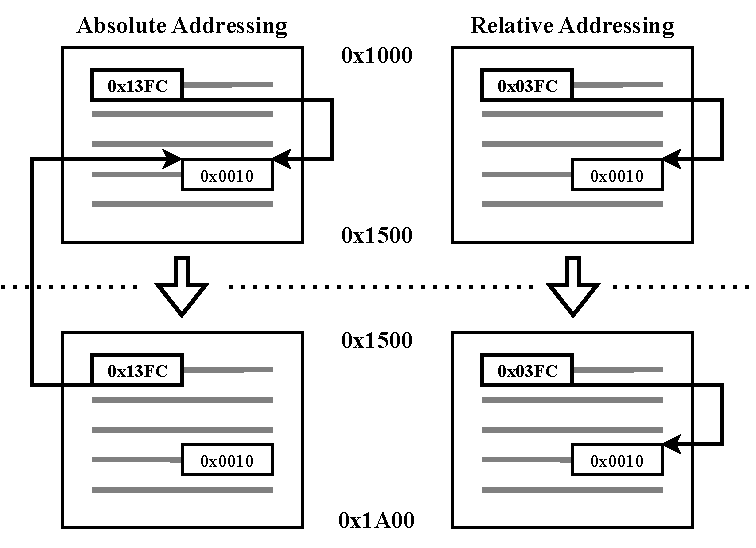
\includegraphics{Figures/Addressing.pdf}
  \caption{Absolute and Relative Addressing.}
  \label{fig:rel_addr}
  \caption*{Two memory blocks with internal self-references. The left one uses absolute addressing, i.e. instructions store the address of the referenced datum, while the right one uses \gls{relative-addressing}, i.e. instructions store the offset from their addresses to the address of the referenced datum. The bottom half of the figure shows what happens when moving both blocks from the address $\mathrm{1000}_{16}$ to $\mathrm{1500}_{16}$ without any further modification. The absolute address reference still points to the old location of the datum, while the relative address reference points to its new location.}
\end{figure}

For sophisticated computer processors~(e.g. those using the \glsxtrshort{Intel} or \glsxtrshort{Arm} \glspl{ISA}), there are typically two classes of addressing modes~\cite{ia32,arm-isa}. Absolute addressing uses memory addresses as described above. \Gls{relative-addressing}, on the other hand, uses memory address offsets that are added to the current instruction address. The advantage of the latter approach is that, if a self-contained memory block referencing its internal data~(e.g. an \gls{image}) is moved to a different start address, this invalidates all internal self-referencing absolute addresses, while all relative addresses remain valid~(see \Cref{fig:rel_addr}). To move memory referenced by an absolute address, it must be updated before dereferencing it again~(see \Cref{sec:reloc}).

\subsection{Memory Pages and Virtual Address Spaces}

To allow for advanced memory management, an abstraction called \gls{virtual-memory} is built on top of \gls{physical-memory}~\cite{os-concepts}. The virtual \gls{address-space} is typically segmented into \glspl{memory-page}, each of which can be individually backed by a different physical \gls{memory-page}, or not be mapped at all~(see \Cref{fig:vmem}). Accesses to unmapped virtual \glspl{memory-page} usually result in a processor exception that can be caught by the operating system. This allows \gls{virtual-memory} to be populated on demand with data from secondary memory, such as persistent storage. \Gls{memory-swapping} is a technique that uses this concept to temporarily offload data from the main memory to persistent storage, particularly in high \gls{memory-contention} situations~\cite{os-concepts,linux-swap}.

\begin{figure}[htb]
  \centering
  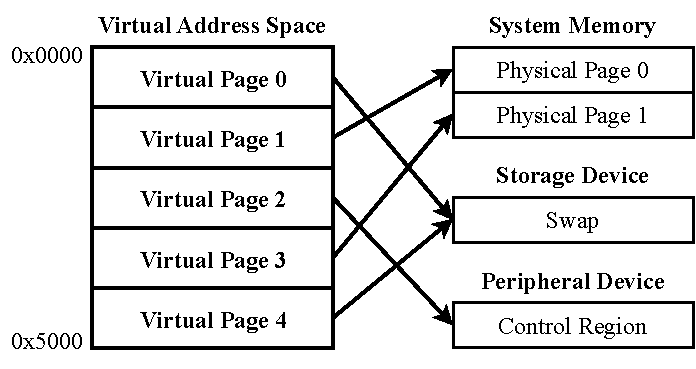
\includegraphics{Figures/VMem.pdf}
  \caption{Virtual Addressing.}
  \label{fig:vmem}
  \caption*{Example of a \gls{virtual-memory} mapping. As shown, \gls{virtual-memory} pages can be mapped to any \gls{physical-memory} page in any order, to a peripheral device \gls{MMIO} region, or to secondary memory such as the \gls{memory-swapping} device. In the latter case, the \gls{virtual-memory} page may be technically unmapped, and the operating system backs it on demand when handling the \gls{page-fault} exception.}
\end{figure}

\section{Memory Allocation Schemes and Memory Management}

\Gls{firmware} implementations and operating system kernels manage platform resources to, among other things, provide drivers and applications with sufficient memory. There are three main approaches to memory allocation. \Gls{static-memory-allocation} reserves fixed amounts of memory with a static lifetime, i.e. it is allocated for the duration of program execution~\cite{ISO:2018:III,rust-ref}. \Gls{call-stack-memory-allocation} allocates~(usually small and fixed amounts of) memory with a local lifetime, i.e. it is allocated exactly while in scope, and it is automatically freed when the scope ends. For this reason, \glsxtrshort{C} also refers to \gls{call-stack-frame} variables as `automatic variables'~\cite{ISO:2018:III}. In contrast, \gls{dynamic-memory-allocation} reserves~(usually large or flexible) amounts of memory with a dynamic lifetime, i.e. it is not limited to a simple scope-based lifetime. \Glsxtrshort{C} requires manual memory management for dynamically allocated memory~\cite{ISO:2018:III}, while the safe subset of \glsxtrshort{Rust} does not support it at all~\cite{rust-ref}.

\subsection{Static Memory Allocation}
\label{sec:static_mem_alloc}

For global data, this is done as part of the initialization of the program and then remains valid throughout its lifetime~\cite{ISO:2018:III,rust-ref}. Essentially, the compiler reserves the memory within the \gls{image} memory~(see \Cref{sec:segments}), there is no runtime memory allocator involved and so there is no room for memory allocation errors.

The size of statically allocated memory is constant, so compilers and code analysis tools know its bounds~\cite{ISO:2018:III,rust-ref}. Because of the static lifetime guarantee, it is not possible to create references to statically allocated memory that may become invalid at runtime. However, references can still become invalid if statically allocated data is available externally, e.g. an exported global variable of a \gls{shared-library}, and the consumers retain references to it after the producer has terminated.

\subsection{Call Stack Memory Allocation}
\label{sec:stack_mem_alloc}

The \gls{call-stack} requires incremental memory allocation for \glspl{call-stack-frame}, i.e. the areas required by specific subroutine calls~(see \Cref{fig:stack})~\cite{os-concepts,ia32,arm-isa}. Unlike \gls{static-memory-allocation}, \gls{call-stack-memory-allocation} requires a memory allocator. The program itself embeds its logic, expanding or shrinking its \gls{call-stack} in a last-in-first-out fashion as needed. While the individual \glspl{call-stack-frame} typically have fixed sizes~(variable-length arrays are a rare exception), unbounded recursions can require infinitely many \glspl{call-stack-frame} and thus infinitely much \gls{call-stack} memory~(except in cases of e.g. \gls{tail-recursion-elimination}~\cite{rec-elim}).

\begin{figure}[htb]
  \centering
  \begin{minipage}{0.35\textwidth}
    \begin{lstlisting}[style=C]
void f(void) {
  uint8_t  f1;
  uint32_t f2;
}

void g(void) {
  uint64_t g1;
  f();
}

void h(void) {
  g();
}
    \end{lstlisting}
  \end{minipage}
  \begin{minipage}{0.5\textwidth}
    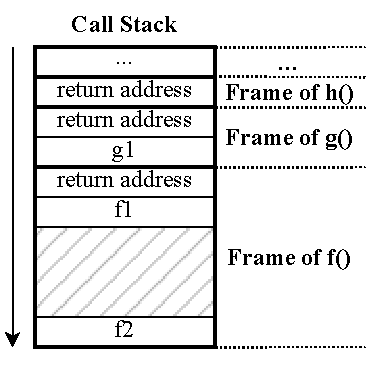
\includegraphics{Figures/CallStack.pdf}
  \end{minipage}
  \caption{Call Stack and Call Stack Frames.}
  \label{fig:stack}
  \caption*{A source code example and the corresponding \gls{call-stack} layout. The \gls{call-stack} generally grows from top to bottom in a last-in-first-out fashion and consists of successive \glspl{call-stack-frame} of subroutine calls. The data within a \gls{call-stack-frame} are aligned according to the \gls{ABI} alignment requirements, i.e. the compiler is likely to insert \gls{data-structure-padding} between \lstinline|f1| and \lstinline|f2|~(the illustration assumes \gls{natural-data-alignment}). The \glspl{call-stack-frame} may have stricter \gls{data-alignment} requirements~\cite{sysVAMD64}, e.g. to satisfy the requirements of vector instructions~\cite{ia32} on \gls{call-stack} memory. In a conventional control flow, each \gls{call-stack-frame} contains the \gls{return-address} of the instruction following the subroutine call.}
\end{figure}

Memory allocation errors are possible when running out of \gls{call-stack} memory, although software engineering best practices aim to make this unlikely~\cite{misra-2012}. With known upper bounds on all recursions and in the absence of variable-length arrays with unknown upper bounds, a reasonable upper bound on the \gls{call-stack} memory requirement can be computed. This allows the \gls{call-stack} size to be chosen accordingly to ensure that it is sufficient for worst-case executions. Unlike with \gls{static-memory-allocation}, references can become invalid at runtime, if they are live when their scope ends~\cite{ISO:2018:III}. A common example of this is returning a reference to a local variable.

\subsection{Heap Memory Allocation}
\label{sec:heap_mem_alloc}

\Gls{heap-memory} allocation, also known as \gls{dynamic-memory-allocation}, reserves memory with a dynamic lifetime from \gls{heap-memory}~\cite{os-concepts,ISO:2018:III,rust-ref}. Dynamically allocated memory remains valid regardless of scope~(including the entry point of the program for some environments) and must be manually freed. It is typically used with variable-size or large amounts of memory. Unlike the schemes discussed previously, dynamically allocated memory is not necessarily live until the end of its scope~(i.e. the end of the block in which it was declared), so intermediate memory can be freed as needed~\cite{ISO:2018:III}. Also, subroutines can return dynamically allocated memory, transferring ownership of it without creating a copy. These points can contribute to lower peak and average memory consumption. On the other hand, \gls{dynamic-memory-allocation} requires a complicated memory allocator~(e.g., the SLUB allocator~\cite{slub-alloc}). By its very nature, heap memory tends to become fragmented over time, which can reduce performance and efficiency for future allocations~\cite{slub-alloc}. To mitigate these problems, real-world operating system algorithms attempt to reduce and avoid fragmentation through means such as overallocation.

There is no general method to derive reasonable upper bounds for memory consumption among other metrics with \gls{dynamic-memory-allocation}. Even if there were, \gls{heap-memory} fragmentation can gradually reduce the effective space available. Thus, it is generally not feasible to provide worst-case guarantees, which is why some embedded systems prohibit \gls{dynamic-memory-allocation} altogether, especially when they have to operate in real-time~\cite{rt-dynmem}. References to dynamically allocated memory may become invalid if they are live after the memory has been freed~\cite{ISO:2018:III}.

\subsection{Memory Safety Violations}
\label{sec:mem_violations}

Because memory is a shared medium, any memory safety violation can have serious consequences. Especially in \gls{kernel-space} or \gls{firmware} contexts, rogue reads can expose secrets and rogue writes can hijack the control flow. The following is a brief description of the main classes of memory safety violations.

\subsubsection{General Memory Safety Violations}

All memory allocations have fixed bounds and are subject to the same data type rules. As such, there are common memory safety violations that are independent of the memory allocation scheme.

\begin{itemize}
  \item \textbf{\Gls{buffer-overflow}:} Accessing a memory buffer outside its allocated range. This may result in reads or corruption of subsequent memory.
  \item \textbf{\Gls{null-pointer-dereference}:} Dereferencing a \lstinline[style=c]{NULL}-pointer. While this can happen in any context, \gls{dynamic-memory-allocation} is one of the most important sources of valid \lstinline[style=c]{NULL}-pointers~\cite{ISO:2018:III}. In particular, low-level software may map the \gls{memory-page} containing the \lstinline[style=c]{NULL} address~\cite{edk2}. In this case, the consequences are similar to \gls{use-after-free}~(see \Cref{sec:dyn_mem_viol}). The inventor of the \lstinline[style=c]{NULL}-pointer, Tony Hoare, has called this his `billion-dollar mistake'~\cite{null-ref-presentation}.
\end{itemize}

\subsubsection{Call Stack Memory Safety Violations}

\Gls{call-stack-memory-allocation}, despite having no dynamic layout logic for its allocation scheme, features a unique safety violation. This is particularly relevant for \glsxtrshort{C} programs, as the compiler automatically manages the allocation and lifetime of \gls{call-stack} variables, but does not provide any safety guarantees.

\begin{itemize}
  \item \textbf{\Gls{use-after-scope}:} Accessing a \gls{call-stack} variable after its scope has ended. Due to automatic scope-based memory management, this immediately invalidates any reference to it.
  \item \textbf{\Gls{call-stack-overflow}:} A \gls{buffer-overflow} with the \gls{call-stack} memory. This is special because the \gls{call-stack} stores the \gls{return-address} for the current function call. Successfully overwriting it may allow the execution of arbitrary code, depending on the platform's security mitigations.
\end{itemize}

\subsubsection{Dynamic Memory Safety Violations}
\label{sec:dyn_mem_viol}

\Gls{dynamic-memory-allocation} safety violations are among the most common and critical vulnerabilities in the software industry~\cite{buff-ovf}. For \glsxtrshort{C} programs, it is particularly prone to human error due to manual lifetime management and limited analysis capabilities of the compiler.

\begin{itemize}
  \item \textbf{\Gls{use-after-free}:} Accessing a reference to previously dynamically allocated memory. If the address has been reused for new dynamically allocated memory, accessing the reference may read or corrupt unexpected memory.
  \item \textbf{\Gls{double-free}:} Freeing a reference to previously dynamically allocated memory again. Depending on the implementation of the dynamic memory allocator, this may corrupt its metadata.
\end{itemize}

\section{Malware and Software Security}

The classic example of a software attack is malware, which must be actively run on the target computer. It can freely execute code and can perform any action that is allowed within the \gls{user-space}, or potentially the sandbox, in which it was executed. While this is one of the simplest methods of a software attack, it requires conscious user interaction and is limited by the privileges of the environment in which it is invoked. In the past, malware had a relatively simple way of getting into the \gls{kernel-space} by asking the user to grant elevated privileges and install a \gls{kernel-space} driver. However, modern operating systems such as Windows, macOS, and Linux derivatives support \gls{kernel-space} driver \gls{digital-signature} authentication~(see \Cref{sec:image_auth}) in combination with \gls{secure-boot}~(see \Cref{sec:sb_mb}). This means that user-initiated privilege escalation alone is no longer sufficient to penetrate the \gls{kernel-space}. Recent versions of macOS on \glsxtrshort{Apple} silicon even require the user to enable loading of third-party \gls{kernel-space} drivers by booting into a special recovery environment, regardless of the driver's \gls{digital-signature}~\cite{macOS-security-settings}.

Despite the best efforts to improve the security of operating systems and firmware, \glsxtrshort{UEFI} malware still appears from time to time~\cite{eset-lojax,blacklotus}. To help combat this growing threat, we must first understand the very basics of common software exploits.

\section{Memory Exploits}
\label{sec:mem_exploits}

Software exploits are a way of further attacking the \gls{kernel-space} and are usually stealthy. Rather than tricking the user into granting elevated privileges, they aim to trigger bugs in software~(including \gls{kernel-space} drivers) that have or are expected to gain elevated privileges. A common family of attack vectors are the memory safety violations~(see \Cref{sec:mem_violations}) discussed earlier. A particularly interesting development in attacks is the move towards \gls{ROP}.

One of the first sophisticated and widespread attacks was \gls{call-stack-smashing}, a technique for corrupting the \gls{call-stack} with attacker-controlled data~\cite{10.1007/978-3-642-33338-5_5}. Using \glspl{call-stack-overflow}, it was previously possible to place \gls{shellcode} on the \gls{call-stack}. By overwriting the \gls{return-address} of the current \gls{call-stack-frame}, the attacker could direct the control flow to that \gls{shellcode} to execute malicious code. In response, operating system kernels marked all \gls{call-stack} memory as non-executable~(see \Cref{sec:mem_perms}).

\Gls{return-to-libc} is a spiritual successor proposed to work around the non-executable \gls{call-stack}. It still relies on overwriting the current \gls{return-address}, but instead of jumping to code controlled by the attacker, it targets code already in memory, so-called \glspl{code-gadget}. One of the most common targets was \gls{libc}, as it is loaded into the \gls{address-space} of almost all \gls{user-space} programs. As part of the demonstration of such an exploit, the reporter proposed the mitigation to fix \gls{call-stack-overflow} attacks based on zero-terminated \gls{ASCII} operations~\cite{libc-zero-byte}. However, it was successfully bypassed by using the \glsxtrshort{PLT}, which was not affected by the mitigation~\cite{libc-ex}.

As the defences grew stronger, the attacks became more versatile, expanding their scope beyond \gls{libc} to other common \glspl{shared-library} as a source of \glspl{code-gadget}~\cite{10.1007/978-3-642-33338-5_5}. In order to exploit even small memory safety violations, sophisticated techniques have been developed to chain \gls{code-gadget} calls. These are now known as \gls{ROP}.

While other families of memory exploits exist, such as \gls{heap-memory} and \glspl{format-string} attacks, they are not fundamentally different from the techniques discussed here. However, they dramatically expand the attack surface for memory exploits. Research conducted by leading low-level security teams has shown that memory exploits are by far the largest class of serious security vulnerabilities~\cite{10.1007/978-3-642-33338-5_5,mem-tag,gpz-zero-days,apple-mem-alloc}.

\section{Image File Formats}

\Glspl{image} capture memory content, layout, and state. They make it easy to bootstrap the program part of a process \gls{address-space}~\cite{levine2000linkers}. The executable part of an \gls{image} carries the program code, while the data part supports \gls{static-memory-allocation}, as discussed earlier~(see \Cref{sec:static_mem_alloc}). Because the common \gls{image-file} formats serve very similar purposes, there have been various design conventions and common concepts between them. These cover both the data structures used to describe the components of and the operations on the \gls{image-file} and \gls{image} \gls{address-space} itself. From them, a kind of abstraction can be sketched as follows.

\subsection{Image File Parsing and the Image File Header}

\Glspl{image-file} are generally header formats, meaning that they start with a data structure called \gls{image-file-header}, which contains information on how to interpret the rest of the file~(see \Cref{fig:img_hdr})~\cite{levine2000linkers}. This includes information such as the \gls{image-base-address}~(see \Cref{sec:reloc}), the offset of the \gls{image-file-section} table~(see \Cref{sec:sections}), and the offset of the \gls{image-segment} table ~(see \Cref{sec:segments}). To easily distinguish between file formats, the \gls{image-file-header} usually starts with a multi-\gls{byte} \gls{file-magic-number}, a constant value to uniquely identify the format. There are also usually means to support newly introduced features while maintaining backward compatibility, such as version numbers, feature flags, and data structure size information.

\begin{figure}[htb]
  \centering
  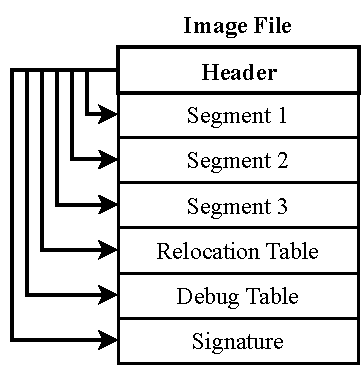
\includegraphics{Figures/Header.pdf}
  \caption{Image File Header.}
  \label{fig:img_hdr}
  \caption*{The \gls{image-file-header} is the data structure at the beginning of an \gls{image-file} that provides information about the rest of the data. It usually identifies the \gls{image-file} format with a \gls{file-magic-number}. From there, it indexes \glspl{image-segment}, \glspl{image-file-section}, the \gls{image-relocation} and debug tables, and optionally the \gls{digital-signature}.}
\end{figure}

In general, \gls{image-file} format designs work in such a way that they can be parsed by interpreting their control data as \glsxtrshort{C} structs~\cite{elf-spec,macho-spec,pe-format}. Using pointer or address arithmetic, the various offsets in the \gls{image-file-header} can be used to access different data structures containing information on how to interpret or process the data. In the following, we will discuss \gls{image-file-loading}, \gls{static-linking}, \gls{dynamic-linking}, and \gls{image-relocation} as examples of operations on \glspl{image-file} and \glspl{image}, along with the data structures that enable them.

\subsection{Image File Loading and Image Segments}
\label{sec:segments}

\Glspl{image} owe their name to the fact that they capture the content and state of memory~\cite{levine2000linkers}. The main tool for this purpose is \glspl{image-segment}~(for \glsxtrshort{PE} files, \glspl{image-file-section} and \glspl{image-segment} are a joint concept~\cite{pe-format}). They describe how to set up both the content of the \gls{image} \gls{address-space}~(e.g. copy or map memory from the \gls{image-file} or initialize with zero-values)~(see \Cref{fig:img_segs}) and its \gls{memory-permissions}~\cite{elf-spec,macho-spec,levine2000linkers}. As such, they are most relevant to \gls{image-file-loading} and execution.

\begin{figure}[htb]
  \centering
  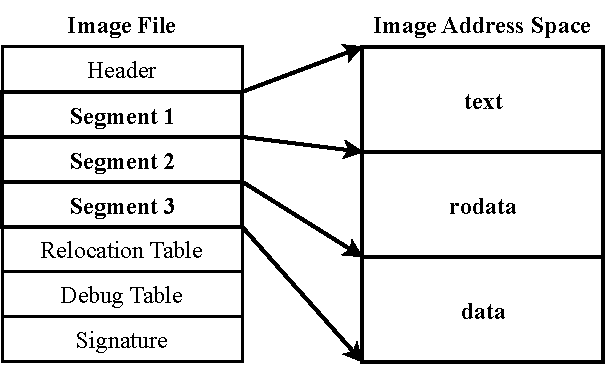
\includegraphics{Figures/Segments.pdf}
  \caption{Image Segments.}
  \label{fig:img_segs}
  \caption*{\Glspl{image-segment} compose the entire \gls{image} \gls{address-space}, both in terms of content and state~(e.g. \gls{memory-permissions}). In general, they do not logically organize content, but group it by their kind~(e.g. executable code, immutable data, mutable data, etc.).}
\end{figure}

Historically, the two most important \glspl{image-segment} are \texttt{text} and \texttt{data}. The former conventionally carries executable code, while the latter holds non-executable data, in particular statically allocated global variables~(see \Cref{sec:static_mem_alloc})~\cite{elf-spec,macho-spec,levine2000linkers}. In addition, \texttt{bss} stores uninitialized global variables~(implicitly defined as a zero-value in \glsxtrshort{C}~\cite{ISO:2018:III}, among other languages) and generally does not occupy space in an \gls{image-file}, because it is initialized to all zero-values at load-time. Finally, to improve memory security, \texttt{rodata} was introduced to mitigate exploits such as overwriting \gls{format-string} literals by enforcing immutability. An alternative approach is to include read-only data in the \texttt{text} \gls{image-segment}~(see \Cref{sec:merge_ro_x}), which is also read-only~(see \Cref{sec:mem_wxorx}).

\Gls{image-file-loading} is the process of transforming an \gls{image-file} into an \gls{image} \gls{address-space}~\cite{levine2000linkers}. In conjunction with \gls{virtual-memory} management, modern operating systems usually just memory-map the \glspl{image-segment} from the \gls{image-file} on the secondary storage into the process \gls{address-space}. \Gls{image-segment} components that are modifiable, such as \glsxtrshort{GOT}, work via \gls{COW} semantics. However, \gls{firmware} implementations, most notably \glsxtrshort{UEFI}, generally do not support \gls{virtual-memory} management and instead copy the data explicitly into the main memory~\cite{pi-spec,uefi-spec,edk2}.

To efficiently compose \glspl{image-segment}, \gls{image-linker} use \glspl{image-file-section} to categorize different types of data and code~\cite{levine2000linkers}. We will explain this composition process in more detail below.

\subsection{Image File Static Linking and Image Sections}
\label{sec:sections}

\Glspl{image-file-section} are units to logically organize the data of an \gls{image}~(see \Cref{fig:img_secs})~\cite{elf-spec,macho-spec,pe-format,levine2000linkers}. For \glsxtrshort{ELF}, \glsxtrshort{MACHO}, and \glsxtrshort{COFF} files, this can be a very granular organization, depending on the build toolchain. For example, \glsxtrshort{MACHO} \glspl{executable-file} generated by the \glsxtrshort{Apple} Xcode toolchain have a dedicated \texttt{cstring} \gls{image-file-section} for string literals~\cite{macho-spec}. \Glsxtrshort{ELF} compilers may generate \glspl{object-file} that go as far as having an \gls{image-file-section} per function and global datum to enable dead code and data garbage collection and improving locality~\cite{gcc}. \Glspl{image-file} of both formats generally have \glspl{image-file-section} for \gls{image-relocation-fixup} and \gls{image-symbol} table information~\cite{elf-spec,macho-spec}. For \glsxtrshort{PE} files, the organization is generally not granular, as they double as \glspl{image-segment}~(see \Cref{sec:segments})~\cite{pe-format}.

\Gls{static-linking} combines several \glspl{image-file} into a joint \gls{library} or \gls{executable-file}~\cite{levine2000linkers}. As suggested earlier, the \gls{image-linker} can use information about references to an \gls{image-file-section} to garbage-collect dead code and data. Not considering the specific configuration, \gls{static-linking} essentially merges all data structures, including \glspl{image-segment}, \glspl{image-file-section}, and \glspl{image-relocation-fixup}. One use case is to include \glspl{static-library}, which is a consumable collection of useful functions and data, within an \gls{executable-file}.

One notable implication is that, if multiple \glspl{executable-file} consume the same function or datum, it will be duplicated across the processes' \glspl{address-space}~\cite{levine2000linkers}. To mitigate this, where beneficial, we will now introduce the concept of \gls{dynamic-linking}.

\begin{figure}[htb]
  \centering
  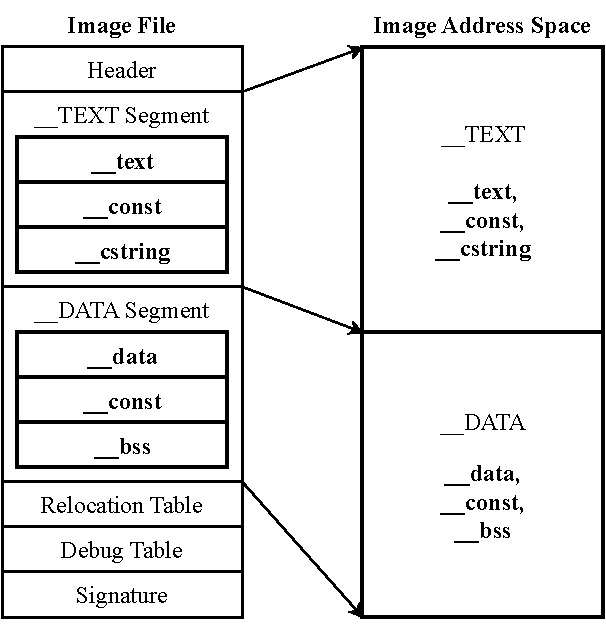
\includegraphics{Figures/Sections.pdf}
  \caption{Image File Sections.}
  \label{fig:img_secs}
  \caption*{The data that make up an \gls{image-segment} are bundled into chunks managed by \glspl{image-file-section} so that the \gls{image-linker} can flexibly move, rearrange, and merge them at link-time. This has several advantages, from garbage collection of unreachable code and unreferenced data to optimization of the binary layout.}
\end{figure}

\subsection{Image Dynamic Linking and Image Symbols}
\label{sec:dyn_link}

\Gls{user-space} programs usually share a lot of code. The most prominent example is \gls{libc}~\cite{gcc}, but operating systems also provide various \glspl{API} to handle user, hardware, and software interaction. To include this shared code in each program individually would result in huge binaries and potentially cause caching problems, as frequent accesses to the same code and data technically target different memory.

To efficiently share code between programs, \glspl{shared-library} complement \glspl{static-library} and \gls{dynamic-linking} complements \gls{static-linking}~\cite{levine2000linkers}. Essentially, only one copy of the \gls{shared-library} is loaded into the main memory, and any dependent \glspl{image} do not resolve their dependencies on it at build-time, but at load-time or runtime. This works by indexing \glspl{image-symbol}, which are essentially named addresses of functions and global data. Dependencies can instruct the \gls{dynamic-linker} to resolve the address of the symbol and adjust the \gls{image} memory to reference it, similar to \glspl{image-relocation-fixup}. Typically, a common data structure can describe both \gls{dynamic-linker} instructions within the \gls{image-relocation} table~\cite{elf-spec,macho-spec}.

\Gls{dynamic-linking} can be done eagerly or lazily~\cite{levine2000linkers}. In the former case, the load time of the program increases, because the \gls{dynamic-linker} resolves all \glspl{image-symbol} even if they may never be accessed during the lifetime of the \gls{image}. In the latter case, function references can be resolved the first time they are used by implementing a stub indexed by the \glsxtrshort{PLT}. However, this requires the resolution targets to be writable at runtime. Thus, high-security configurations typically force the use of eager \gls{dynamic-linking}.

Since every executable \gls{address-space} is different, there is no way to guarantee that the \gls{image-base-address} of a \gls{shared-library} will be available across all of its consumers~\cite{ms-dll-base-addr}. Furthermore, avoiding predictable addresses can be a powerful tool for making memory exploits less reliable. The solution to both is \gls{image-relocation}, which we will discuss next.

\subsection{Image Relocation and Position-Independence}
\label{sec:reloc}

Modern operating systems have complex requirements for the dynamic loading of \glspl{shared-library}, drivers, and applications. This includes the ability to load \glspl{image} at arbitrary addresses~(see \Cref{sec:dyn_link}). This can also be used to increase resilience against various software exploits by using \gls{pseudo-randomization} for the load address of \glspl{image} as part of \gls{ASLR}~\cite{app9142928}. Binaries that support being moved are commonly referred to as \gls{PIC}~\cite{levine2000linkers}. Not all binaries are inherently position-independent, as the compiler may generate \glsxtrshort{CPU} instructions or data with absolute addresses to data within the \gls{image}. This may happen because the target \gls{ISA} has poor support for \gls{relative-addressing}, absolute addressing may be more performant, or there are global pointers-to-pointers initialized at build-time.

A common part of solving the problem of position dependency is the indexing and processing of \glspl{image-relocation-fixup}~(see \Cref{fig:imgreloc})~\cite{levine2000linkers}. In this context, they are instructions to the \gls{image-file-loader} on how to modify \glsxtrshort{CPU} instructions and addresses to execute from a specific address. The \gls{dynamic-linker} links the \gls{image} to run at an address specified at build-time, commonly referred to as the \gls{image-base-address}. \Glsxtrshort{CPU} instructions and addresses that require absolute addressing to data in the \gls{image} get \glspl{image-relocation-fixup} indexed, which tell the \gls{image-file-loader} where and how to update them. \Glsxtrshort{CPU} instructions that do not trivially encode absolute addresses get fixed by \glspl{image-relocation-fixup} that are specific to the host architecture declared by the \gls{image-file-header}~\cite{elf-spec,pe-format,arm64-elf}. The \gls{image-file-loader} then processes the \glspl{image-relocation-fixup} as part of \gls{image-file-loading} by adding the offset of the \gls{image-base-address} and the final load address to the relocatable address in the manner required by the \gls{image-relocation-fixup} type~\cite{levine2000linkers}. In a different context, \gls{static-linking} also uses \glspl{image-relocation-fixup}, but they are typically indexed differently~(i.e. per \gls{image-file-section} rather than for the whole \gls{image}) and have different semantics~(e.g. for \gls{relative-addressing} across \glspl{image-file-section}).

\begin{figure}[htb]
  \centering
  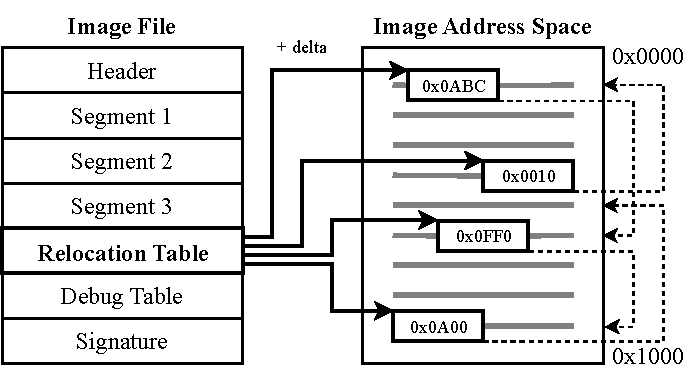
\includegraphics{Figures/RelocFixups.pdf}
  \caption{Image Relocation Fixups.}
  \label{fig:imgreloc}
  \caption*{The \gls{image-relocation} table contains \glspl{image-relocation-fixup} which tell the \gls{image-file-loader} how to update the \gls{image} \gls{address-space} when moving it from the \gls{image-base-address}~(where `delta' is their difference). The dashed lines visualize the absolute addresses that the \glspl{image-relocation-fixup} target within the \gls{image} \gls{address-space}.}
\end{figure}

\Glsxtrshort{UEFI} has adopted this model of dynamic \gls{image-file-loading} to meet its own needs for dynamic driver dispatching and execution of arbitrary applications at operating system runtime~\cite{pi-spec,uefi-spec}. It has also extended it with the notion of \gls{runtime-image-relocation}. This allows the operating system to map memory required by \glsxtrshort{UEFI} during the operating system runtime to non-identity \gls{virtual-memory} addresses. It enables \gls{KASLR} to be extended to include \glsxtrshort{UEFI} runtime memory~\cite{xnu}.

\subsection{Additional Metadata and Extensibility}

Beyond the essential data, \gls{image-file} formats often support some form of metadata extensibility~\cite{elf-spec,macho-spec,pe-format}. This can be debugging information, for example, to help developers with the development process. In general, most \glspl{image-file} formats support special \glspl{image-file-section} with predefined names. However, this requires the metadata to be mapped into the \gls{image} address space, which is not always desirable. Therefore, some formats provide maps of identifiable data structures, which may or may not point to data in the \gls{image} \gls{address-space}~\cite{macho-spec,pe-format}. Some also define \gls{image-file-header} data structures with flexible sizes to ensure extensibility and backward compatibility~\cite{elf-spec}.

\subsection{Image Authentication and Cryptographic Hashes}
\label{sec:image_auth}

For security reasons, operating systems and \gls{firmware} implementations usually authenticate \glspl{image-file}. This ensures that the \gls{image-file} has been approved by a trusted entity and has not been tampered with by a third party. This is achieved by using \glspl{digital-signature}, which leverage asymmetric cryptography to securely sign the \glspl{image-file}. The public key in this scheme can be used to verify that the \gls{digital-signature} is correct and that the \glspl{image-file} is authentic. \Gls{image} authentication is the basis of \glsxtrshort{UEFI} \gls{secure-boot} and \gls{measured-boot}~(see \Cref{sec:sb_mb}).

There are two approaches to \gls{image} authentication. The first is to digitally sign the \gls{image-file} itself. This is a simple scheme that ideally cryptographically hashes the entire file in one piece~(see \Cref{fig:img_file_sig}).

\begin{figure}[htb]
  \centering
  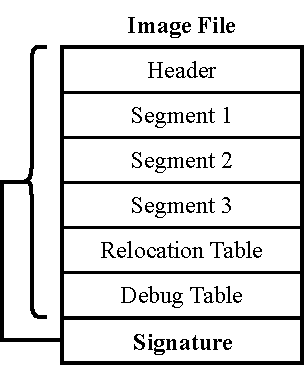
\includegraphics{Figures/Signature.pdf}
  \caption{Digital Signature based on the Image File.}
  \label{fig:img_file_sig}
  \caption*{An \gls{image} authentication scheme that digitally signs the \gls{image-file} itself. It may cover the entire \gls{image-file} or only a subset of it~(e.g. see \Cref{sec:authenticode}). However, it must cover the \gls{image} \gls{address-space} implicitly, i.e. all \glspl{image-segment}, to be secure.}
\end{figure}

Hashing the \gls{image} \gls{address-space}~(see \Cref{fig:img_sig}) has the advantage that it integrates well with the \gls{virtual-memory} approach to \gls{image-file-loading} and \gls{memory-swapping}. Technically, individual \gls{image} \glspl{memory-page} can be lazily loaded many times throughout the lifetime of the \gls{image}. To prevent \gls{TOC-TOU} attacks, they should ideally be authenticated each time they are fetched from secondary memory. One approach to this is to store a data structure containing \glspl{cryptographic-hash} for each memory-mapped \gls{memory-page} of the \gls{image-file} and then digitally sign it. Now, each time a \gls{memory-page} is fetched, its \gls{cryptographic-hash} can be compared to the in-memory copy of the data structure copy to authenticate it quickly and lazily. Since the entire \gls{image-file} is usually memory-mapped, which is pretty much mandatory to take full advantage of \gls{virtual-memory} in this context, this implicitly authenticates the entire \gls{image-file}.

\begin{figure}[htb]
  \centering
  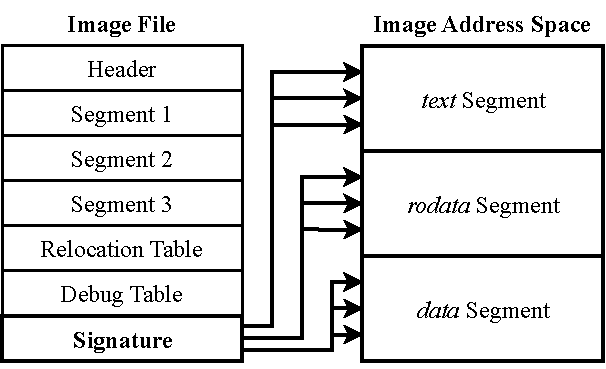
\includegraphics{Figures/SignatureAlt.pdf}
  \caption{Digital Signature based on the Image Address Space.}
  \label{fig:img_sig}
  \caption*{An \gls{image} authentication scheme that digitally signs the \gls{image} \gls{address-space} directly. To enable lazy loading and thus authentication of \gls{image} \glspl{memory-page}, it is particularly useful to store a map of their cryptographic hashes. If the entire \gls{image-file} is memory-mapped, as is typical for \gls{image-file-loading} powered by \gls{virtual-memory}, it is implicitly authenticated as a whole.}
\end{figure}

Similar concepts of nested cryptographic hashing and lazy authentication can be found in the field of filesystems~\cite{apfs}. Because they have a hierarchical structure rather than a flat one, it is desirable to be able to lazily authenticate each level on demand. This is done not just by using two levels of \glspl{cryptographic-hash}, but by computing a tree of them, where a parent hashes the aggregated hashes of all its children~\cite{merkle-trees}. This is known as a Merkle tree, a generalization of the nested cryptographic hashing concept.

\section{Problem Statement and Proposals}
\label{sec:problem_statement}

As we have seen, memory safety violations are a significant and critical threat to system security and parsing in particular is a likely source of them. Current \glsxtrshort{UEFI} \gls{firmware} provides only a few of the state-of-the-art defences employed by operating systems. At the same time, there are tight constraints on the platform code size, such that space efficiency is a valid concern. The \glsxtrshort{UEFI} Forum's previous attempt at a new \gls{executable-file} format in the form of \glsxtrshort{TE} failed to address both security and space efficiency concerns with the existing \glsxtrshort{PE} specification and infrastructure~(see \Cref{sec:te})~\cite{secure-pe}.

In addition, \gls{image-file} modification and conversion are crucial for building \glsxtrshort{UEFI-PI} and \glsxtrshort{UEFI} software, especially for the \gls{EDK2} build system~(see \Cref{sec:img_conv}). However, the existing tools all rely on direct conversion between formats and do not have sufficient testing in place. As a result, the generated \glspl{image-file} are often malformed or insecure~\cite{gnu-efi-fix,ipxe-fix}.

In response, we propose a novel \gls{executable-file} format to reduce the attack surface for parsing errors and bugs, as well as the complexity of the parser itself, while also rethinking the encoding of the metadata to increase the space efficiency. To generate files of this format, we also propose a novel \gls{executable-file} conversion stack that relies on an intermediate representation to abstract and validate the conversion process.

\section{Outline}

After this brief introduction to \glspl{image}, their basic concepts, and the importance of secure parsing, we will now give an outline of this thesis.

\begin{itemize}
  \item First, we will discuss related work in \Cref{chap:related_work}. In particular, we are interested in common real-world \gls{image-file} formats and their design in the context of modern operating systems, our target environment \glsxtrshort{UEFI}, and related safety and security practices.
  \item \Cref{chap:uefi_exec_reqs} begins our contribution with requirements engineering for our proposal of a novel \glsxtrshort{UEFI} \gls{executable-file} format. We will then define an abstraction of \glsxtrshort{UEFI} \glspl{executable-file} from its results and common practices across \gls{image-file} format designs.
  \item We will detail design considerations that combine industry best practices in encoding and parsing with the requirements and guarantees of \glsxtrshort{UEFI}, for such a novel format in \Cref{chap:uefi_exec_design}.
  \item In \Cref{chap:uefi_exec_impl}, we will explain the architecture and principles of the implementation, together with our testing techniques and methodology.
  \item Finally, we will conclude the thesis with our results in \Cref{chap:results}, our conclusion in \Cref{chap:conclusion}, and future work in \Cref{chap:future_work}.
\end{itemize}

%%%%%%%%%%%%%%%%%%%%%%%%%%%%%%%%%%%%%%%%%%%%%%%%%%%%%%%%%%%%%%%%%%%%%%%%%%%%%%%
\chapter{Related Work} %%%%%%%%%%%%%%%%%%%%%%%%%%%%%%%%%%%%%%%%%%%%%%%%%%%%%%%%
\label{chap:related_work}

To get a good understanding of the basics of \glspl{image} and \gls{image-file} formats, we will first discuss common formats used across different operating systems and \gls{firmware} implementations in \Cref{sec:cmn_formats}. We will then look at different types of \gls{image} authentication schemes in \Cref{sec:cmn_sigs}. Next, we will review the state of the art for the related \glsxtrshort{UEFI} technologies and the reference implementation in \Cref{sec:uefi_solutions}. After, we will briefly outline the problems with current \gls{image-file} solutions and showcase an earlier attempt to address them in \Cref{sec:formal_pe}. In \Cref{sec:img_conv}, we will go through existing projects for \gls{image-file} format conversion and what they have in common. Finally, in \Cref{sec:impr_mem_safetym,sec:rust}, we will look at techniques for stress-testing for and guaranteeing memory safety.

\section{Common Image File Formats}
\label{sec:cmn_formats}

For workstations, both home and commercial, and servers, the most common operating systems are \glsxtrshort{Microsoft} Windows, \glsxtrshort{Apple} macOS, and operating system distributions based on the Linux kernel. In the following, we will introduce their respective preferred \gls{image-file} formats and their basic design ideas.

\subsection{Executable and Linkable Format~(ELF)}
\label{sec:elf}

A common \gls{image-file} format for UNIX- and Linux-based operating systems is the \glsxtrfull{ELF}. Formerly specified by the \gls{TIS} Committee~\cite{elf-spec}, it is now managed by \gls{SCO} as part of the System V and other \gls{ABI} specifications~\cite{arm64-elf,sysVGABI,sysVUpdate}. Architecture-specific details of the format, such as specific \gls{image-relocation-fixup} types, are defined separately in the \gls{ISA}-specific \gls{ABI} specifications~\cite{arm64-elf,sysVUpdate,sysVi386}.

The design of the \gls{image-file} format suits the needs of \gls{static-linking}, \gls{dynamic-linking}, and execution. The different views for the two \gls{image} linking scenarios can be seen in \Cref{fig:elf_link_exe}.

\begin{figure}[htb]
  \centering
  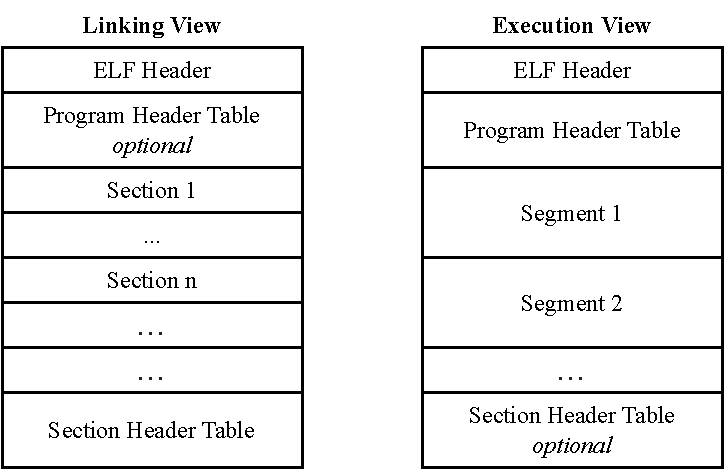
\includegraphics{Figures/ELF.pdf}
  \caption{`Object File Format'~(Figure 1-1.)~\cite{elf-spec}.}
  \label{fig:elf_link_exe}
  \caption*{The \glsxtrshort{ELF} file views for \gls{image} linking compared to execution. \Gls{image} linking is primarily concerned with \glspl{image-file-section}, the smaller building block for \glspl{image-file}. \Glspl{image-file-section} generally categorize types of content. Often, categories such as `debug data' and `string literals' are grouped into a common \gls{image-file-section}. For \glspl{object-file}, they may only cover a single function or datum. \Gls{image} loading and execution work with \glspl{image-segment}, the larger building blocks that are made up of \glspl{image-file-section}. \Glspl{image-segment} generally categorize data into \gls{memory-permissions} groups. For example, this may be `executable code' or `read-only data'. The content of the data is not relevant to \gls{image} execution.}
\end{figure}

\subsubsection{Position-Independence, GOT, and PLT}

Several \glspl{executable-file} can use the same \gls{shared-library}. It must therefore be mapped into all of their respective process \glspl{address-space}. Immutable \glspl{image-segment} will remain the same in all of them. For this reason, operating systems usually load these \glspl{image-segment} only once and map them into all consumer process \glspl{address-space}~\cite{ms-dll-base-addr,xnu,linux}. The Linux kernel in particular makes extensive use of \gls{COW}, a technique for sharing code and data as immutable across arbitrarily many consumers and duplicating it when written to, for such purposes~\cite{linux}. For process \glspl{address-space}, this is implemented by mapping the \gls{memory-page} as read-only and hooking the \gls{page-fault} handler to duplicate it.

Technically, read-only \glspl{image-segment} can still be targeted by \glspl{image-relocation-fixup}. This will cause the same problems as described above for writable \glspl{image-segment} and may duplicate many to most of the associated \glspl{memory-page} via \gls{COW}. To reduce this amount of \glspl{memory-page}, the \glsxtrfull{GOT} was introduced as an indirection for memory accesses to externally linked data~(see \Cref{fig:got})~\cite{levine2000linkers,elf-spec}. By using \gls{relative-addressing} for \glsxtrshort{GOT} accesses, this makes these \glspl{image-segment} truly immutable, and thus they will never be subject to \gls{COW} duplication.

The \glsxtrfull{PLT} follows the same ideas as the \glsxtrshort{GOT}, but it specifically targets executable code~\cite{levine2000linkers,elf-spec}. As an indirection, the \glsxtrshort{PLT} carries stubs for all affected subprocedures.

\begin{figure}[htb]
  \centering
  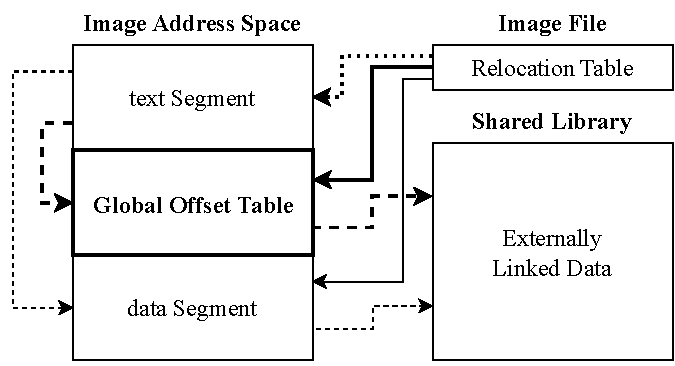
\includegraphics{Figures/GOT.pdf}
  \caption{Image Global Offset Table.}
  \label{fig:got}
  \caption*{The \glsxtrshort{GOT} is an indirection layer to avoid process-specific \glspl{image-relocation-fixup} to read-only \glspl{image-segment}. In particular, it is an indirection for all \gls{image} memory accesses via absolute addresses. In the case of \glspl{PIE}, all accesses to \glsxtrshort{GOT} itself are relative. Different processes can map the same \gls{shared-library} to different load addresses. To account for this, each process has a copy of the \glsxtrshort{GOT} with the absolute addresses corresponding to its own \gls{address-space}. The dotted line visualizes the \glspl{image-relocation-fixup} that allow read-only \glspl{image-segment} to address \glsxtrshort{GOT} or other data strictly within the own \gls{image} \gls{address-space}~(applies only to non-\glspl{PIE}).}
\end{figure}

\subsubsection{RELR and RELRO}

In recent years, RELR has established itself as the most efficient encoding for relative \glspl{image-relocation-fixup} in \glsxtrshort{ELF} to date~\cite{elf-relr}. The idea is to store the address of a relocation target along with a bitmap of adjacent locations to relocate. The idea is to take advantage of the locality of relative \glspl{image-relocation-fixup}, e.g. such as those issued for global pointer arrays.

As mentioned before, lazy \gls{dynamic-linking} requires the \gls{image-relocation} targets to be writable, which may allow attackers to hijack them~(see \Cref{sec:dyn_link}). \Glsxtrshort{ELF}'s solution to this is \glsxtrfull{RELRO}, which, when fully enabled, forces eager \gls{dynamic-linking} and marks \glsxtrshort{GOT} and \glsxtrshort{PLT} as read-only when done~\cite{ld}. Partial \glsxtrshort{RELRO} is supported, but not recommended for security reasons.

\subsection{Mach Object File Format~(Mach-O)}
\label{sec:macho}

The default \gls{image-file} format for \glsxtrshort{Apple} operating systems, such as macOS, iOS, and watchOS, is the \glsxtrfull{MACHO}~\cite{macho-spec}. At a high level, it is very similar to \glsxtrshort{ELF}, especially regarding \gls{PIC}, which is the default mode for the \glsxtrshort{Apple} Xcode toolchain. However, unlike \glsxtrshort{ELF}, which requires features such as \glsxtrshort{RELRO}, initial and maximum protection levels are part of the \glsxtrshort{MACHO} core design for \glspl{image-segment}.

The traditional format for storing \glspl{image-relocation-fixup} in an \gls{image-file} is a table. It can be nested, so that there is a sub-table for each \gls{memory-page} of the \gls{image}, and each such entry has a table of offsets relative to its \gls{memory-page}. \Glsxtrshort{Apple} has introduced a new storage format for \glsxtrshort{MACHO} in recent years, called dyld chained fixups~\cite{dyld_chains}. This is again based on the table format with one sub-table for each \gls{memory-page}. However, the new format stores \glspl{image-relocation-fixup} as a linked list within an \gls{image-segment} at the \gls{image-relocation} target location~(see \Cref{fig:fixup_chains}). This means that the target of an \gls{image-relocation-fixup} stores a data structure that compresses its metadata, as well as the offset to the next \gls{image-relocation-fixup}.

The \glsxtrshort{MACHO} format introduced a constraint on the \gls{image} \gls{address-space} size of $64$~GiB, which requires $\log_2(64 \cdot 1024^3) = 38$~bits to store a valid address in an \gls{image} \gls{address-space} if its \gls{image-base-address} is $0$. Meanwhile, since the chain is per \gls{memory-page}, the offset to the next \gls{image-relocation-fixup} can be at most $4095$ \glspl{byte}, thus requiring $\lceil \log_2(4095) \rceil = 12$~bits to store. Both data require $50$~bits of storage, which easily fits into the original $64$-bit target.

This new organization of \glspl{image-relocation-fixup} can save a significant amount of storage space for \glspl{image-file} with many \glspl{image-relocation-fixup}, as the `free storage space' for \gls{chained-image-relocation-fixups} far outweighs the per-\gls{memory-page} tables of the \gls{image-relocation} table~\cite{dyld_chains}.

Furthermore, their design addresses an issue of temporally separate accesses to the same \glspl{memory-page}, which may require \gls{memory-swapping} during \gls{dynamic-linking}~\cite{dyld_chains}. Namely, \gls{image-relocation} and \gls{dynamic-linking} are unified as a single step for each \gls{image-relocation-fixup}, requiring only a single pass over each \gls{image-segment} \gls{memory-page}.

\begin{figure}[htb]
  \centering
  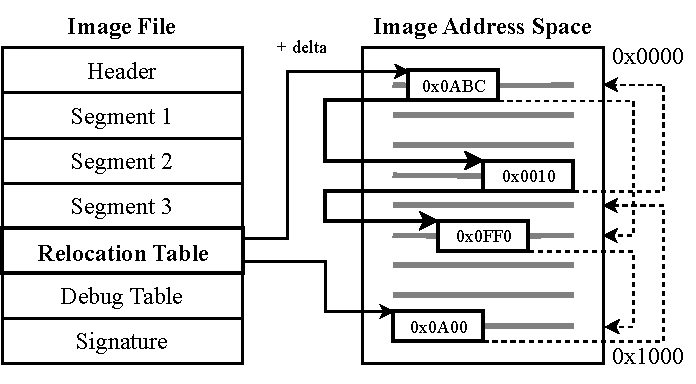
\includegraphics{Figures/FixupChain.pdf}
  \caption{Image Relocation Fixup Chains.}
  \label{fig:fixup_chains}
  \caption*{Similar to \Cref{fig:imgreloc}, but singly-linked chains organize the \glspl{image-relocation-fixup}. As all the necessary information resides in the \gls{image-relocation} target, this helps to reduce the size of the \gls{image-file} and decreases the number of memory accesses outside the same \gls{memory-page}. This is implemented by the \glsxtrshort{MACHO} format for \glspl{image-relocation-fixup} of the same type within the same \gls{memory-page}.}
\end{figure}

\subsection{Portable Executable and Common Object File Format~(PE/COFF)}
\label{sec:pecoff}

For the \glsxtrshort{Microsoft} Windows operating system, \glsxtrshort{Microsoft} primarily uses the \glsxtrfull{PECOFF}~(see \Cref{fig:pe_layout})~\cite{pe-format}. It is also the primary format specified by the \glsxtrshort{UEFI-PI} and \glsxtrshort{UEFI} specifications~\cite{pi-spec,uefi-spec}. Unlike \glsxtrshort{ELF} and \glsxtrshort{MACHO}, \glsxtrshort{PECOFF} combines the concepts of \glspl{image-segment} and \gls{image-file-section} under the latter's name~\cite{pe-format}.

\begin{figure}[htb]
  \centering
  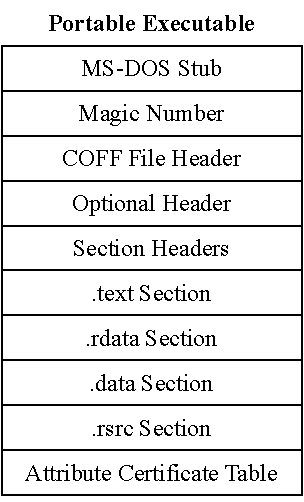
\includegraphics{Figures/PE.pdf}
  \caption{Portable Executable File Organization.}
  \label{fig:pe_layout}
  \caption*{Example \glsxtrshort{PE} file layout. The MS-DOS stub is virtually unused and is only a relic for backward compatibility. Due to the dual nature of \glsxtrshort{PE} and \glsxtrshort{COFF} files, there are separate data structures to describe metadata for both use cases, namely the Optional Header and the COFF File Header. The multiple layers of headers add to the complexity of \glsxtrshort{PE} parsing~\cite{secure-pe,audk}. The \glspl{image-file-section} double as \glspl{image-segment}. Optionally, there is a trailing certificate table that contains \glspl{digital-certificate}.}
\end{figure}

To compress the \gls{image-relocation} directory, \glsxtrshort{PE} introduced the concept of Base Relocation Blocks~\cite{pe-format}. They consist of a $4$ KiB aligned base address within the \gls{image} \gls{address-space} and a variable-size list of Base Relocations~(\glspl{image-relocation-fixup}). By indexing the \glspl{image-relocation-fixup} per $4$~KiB block, they only store their offset within the block, which requires only $12$~bits instead of the $32$ or $64$~bits needed for a full address.

\subsubsection{Caveats}

\Glsxtrshort{PE} suffers from dangerous data duplication, e.g. it has several \lstinline|SizeOf*| fields, such as \lstinline|SizeOfImage|, with sums of certain or all  kinds of \glspl{image-segment} sizes~\cite{pe-format}. Relying only on their values alone may cause \glspl{buffer-overflow} if they do not match reality~\cite{secure-pe}. However, to validate them, one needs to recompute the values from the \gls{image-segment} information. Therefore, for many use cases, it may be best to ignore these fields, as done by the \gls{AUDK} \glsxtrshort{PE} loader~\cite{audk}.

There are also unintuitive design choices that confused reviewers of the `Securing the EDK II Image Loader' publication~\cite{secure-pe}. For example, the number of \glspl{image-relocation-fixup} within a block must always be even~\cite{secure-pe}. This is, because \glspl{image-relocation-fixup} information has a \gls{data-alignment} requirement of $2$ \glspl{byte}, while blocks must start on a $4$~\gls{byte} boundary~\cite{pe-format}. An odd amount of \glspl{image-relocation-fixup} must be padded with another of type \lstinline|IMAGE_REL_BASED_ABSOLUTE|, which is skipped during \gls{image-relocation}.

\subsubsection{Backward Compatible Position-Independence}

The notion of \gls{PIC} is different for the \glsxtrshort{PE} format compared to \glsxtrshort{ELF} and \glsxtrshort{MACHO}. \Glspl{image-relocation-fixup} can target read-only \glspl{image-segment} even for \glsxtrshort{PE} \glspl{shared-library}, which means that, unlike their counterparts in the other formats, most of their \glspl{memory-page} could not be shared if they were loaded at different load addresses across process \glspl{address-space}~\cite{ms-aslr}. Note that not sharing significant portions of \gls{shared-library} memory removes most of the benefits of the concept.

With the introduction of \gls{ASLR}, the Windows kernel started pseudo-randomizing the load address of \glspl{shared-library} and \gls{executable-file}~\cite{ms-aslr}. Before the introduction of \gls{ASLR}, this was the \gls{image-base-address} and collisions caused an \gls{image-relocation} of the \gls{shared-library} and thus creating a copy. For this reason, \glspl{image-base-address} used to be carefully chosen to minimize the risk of collisions between process \glspl{address-space}. To avoid requiring changes to the existing design of \glspl{shared-library}, and to mitigate the \gls{COW} penalty mentioned above, it still tries to load multiple instances of a \gls{shared-library} at the same load address across all processes~\cite{ms-dll-base-addr}. To do this, it keeps track of the previous \gls{ASLR} allocations and only draws the address from the available ranges. The \gls{image-file} is then fixed up when it is loaded from secondary memory, so that it appears to the rest of the existing \gls{shared-library} stack as if the \gls{image-base-address} was the \gls{ASLR} address, and it happened to be available. In case of a collision, the \gls{shared-library} still needs to be duplicated, but this is not a regression from the previous design. On the contrary, the \gls{pseudo-randomization} reduces the risk of collisions compared to the previous manual optimization.

This approach has the obvious disadvantage that one process can learn information about another's \gls{address-space} via a \gls{side-channel}. It also has to explicitly handle the case of an address collision, unlike \glsxtrshort{ELF} and \glsxtrshort{MACHO}, potentially leading to increased memory consumption~\cite{ms-dll-base-addr}. Support for \gls{PIC} as implemented by the other formats has not been added to the \glsxtrshort{PE} specification or \gls{MSVC}~\cite{pe-format}.

\subsection{Merging Read-Only Data with Executable Code}
\label{sec:merge_ro_x}

To reduce the impact of increased memory space requirements due to \gls{memory-page} boundary padding when tightening \gls{memory-permissions}, some build systems merge read-only data with executable code on the same \gls{memory-page}~\cite{macho-spec,edk2}. This preserves immutability, meaning that the affected data cannot be corrupted to hijack the control flow. This is particularly important, because \glspl{static-memory-allocation} can affect computations, or the control flow directly, e.g. lookup tables, function tables, and so on.

At the same time, the more executable code there is, the more likely there is to be a suitable \gls{code-gadget} naturally increases. Unfortunately, we have not been able to find any meaningful research on the impact of this.

\section{Common Image Authentication Schemes}
\label{sec:cmn_sigs}

To support \gls{image} authentication at a scale, several approaches have emerged for the \gls{kernel-space} and \gls{user-space} environments. In the following, we will look at the state of the art in operating system designs.

\subsection{Linux Module Signature Format}

\Glsxtrshort{ELF} does not currently support \glspl{digital-signature}~\cite{elf-spec}. \Gls{user-space} applications and \glspl{library} are generally not digitally signed. To work around this limitation, the Linux kernel introduced the Linux Module Signature Format~(see \Cref{fig:linux_sig})~\cite{linux}. This is a trailer-based format independent of \glsxtrshort{ELF} that is appended to a Linux module to digitally sign it. The \gls{digital-signature} covers the whole \gls{image-file}~(see \Cref{fig:img_file_sig})~\cite{linux}.

Unfortunately, this introduces a slight ambiguity that is not trivial to resolve. Namely, the \gls{image-file-loader} could process any Linux Module that has the Linux Module Signature Format \gls{file-magic-number} at the end, e.g. as an unrelated datum at the end of its last \gls{image-file-section}, as if it were digitally signed, even if it is not. To mitigate this, the Linux module needs to have some information about its file size, which for \glsxtrshort{ELF} files can only be obtained by parsing the \gls{image-file-section} table~\cite{elf-spec}. While this is unlikely to cause any security or real-world usability problems in practice, it may be relevant for possible formalization efforts in the future.

\begin{figure}[htb]
  \centering
  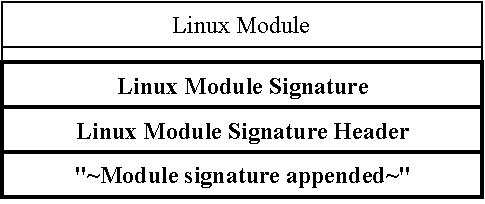
\includegraphics{figures/LinuxSig.pdf}
  \caption{Linux Module Signature Format~\cite{linux-kmod-sig}.}
  \label{fig:linux_sig}
  \caption*{The Linux Module Signature Format is trailer-based and independent of \glsxtrshort{ELF}. The trailer \gls{file-magic-number} \lstinline{\"\~Module signature appended\~\"} identifies a Linux Module to which a \gls{digital-signature} has been appended. The \gls{file-magic-number} is preceded by the \gls{digital-signature} header, which contains the information needed to process the \gls{digital-signature}, such as the \gls{cryptographic-hash} function and the \gls{digital-signature} size. Finally, the actual \gls{digital-signature} is located before the header.}
\end{figure}

\subsection{Code Directory Hash and Image4 Signature Formats}
\label{sec:cdhash}

\Glsxtrshort{Apple} operating systems generally use the Code Directory Hash~(cdhash) \gls{digital-signature} format for \gls{user-space} applications and \glspl{library}~\cite{apple-cdhash,apple-cdhash-old}. It stores a data structure with a \gls{cryptographic-hash} for each \gls{memory-page} of the \glsxtrshort{MACHO} \gls{image}, as this allows code authentication when loading them lazily during execution~(see \Cref{fig:img_sig}).

For the boot process, including \gls{secure-boot}, \glsxtrshort{Apple} platforms use their proprietary Image4 format~\cite{xnu,opencore}. Like the Linux Kernel Module Signature Format, it hashes the module as a whole. However, it is not just a simple appended \gls{digital-signature}, but a sophisticated dictionary of various data stored in a separate file. For example, it may contain a unique machine identifier to allow personalized \glspl{digital-signature}.

\subsection{Authenticode PE Signature Format}
\label{sec:authenticode}

\Gls{authcode} is used by \glsxtrshort{Microsoft} for its operating systems, most notably Windows~\cite{pe-authenticode}. It is also the scheme adopted by the \glsxtrshort{UEFI} specification for \gls{secure-boot}, as there is no viable alternative for \glsxtrshort{PE} files. It is by far the most complicated \gls{image} authentication scheme out of the four we cover~(see \Cref{fig:authcode}), while at the same time not integrating well with \gls{virtual-memory}. The hashing algorithm skips over some data in the \gls{image-file-header} and its implementation for \glspl{executable-file} used to tolerate trailing data~\cite{jar-msi-auth-bug}. Part of its complexity is to increase debugging flexibility~\cite{pe-authenticode}, but it also significantly weakens its security properties. There have been several theoretical and practical attacks against this \gls{image} authentication scheme, targeting both Windows and \glsxtrshort{UEFI} implementations~\cite{secure-pe,jar-msi-auth-bug,mic-auth-bug,win-auth-bug,uefi-auth-bug}.

\begin{figure}[htb]
  \centering
  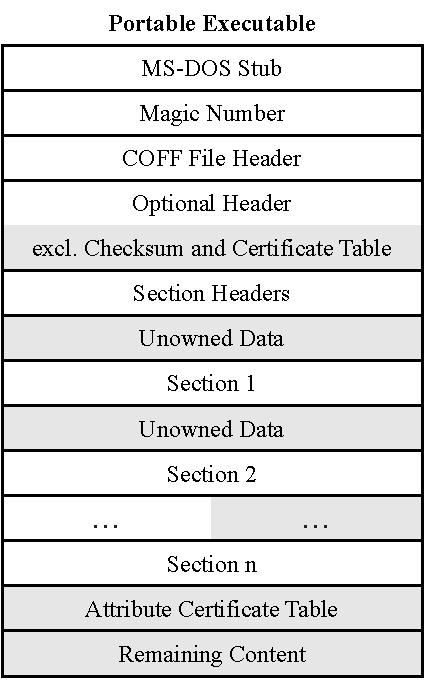
\includegraphics{Figures/AuthCode.pdf}
  \caption{PE File Coverage by the Authenticode Scheme.}
  \label{fig:authcode}
  \caption*{The \glsxtrshort{PE} data covered by the \gls{authcode} hash scheme. It cryptographically hashes data with a white background but not data with a grey background. `Unowned Data' refers to data that is not covered by any \glsxtrshort{PE} \gls{image-file-section} or data structure. In particular, any data following the Attribute Certificate Directory is not part of the \glsxtrshort{PE} \gls{authcode} \gls{cryptographic-hash}~\cite{pe-authenticode}.}
\end{figure}

\section{UEFI Solutions and Reference Implementations}
\label{sec:uefi_solutions}

Now that we have looked at the state of the art in operating system designs, let us discuss the status quo and the solutions offered by the \glsxtrshort{UEFI} \gls{firmware} ecosystem. In particular, this includes an attempt by the \glsxtrshort{UEFI} Forum to establish an \gls{image-file} format for the \gls{firmware} space.

\subsection{Terse Executable File Format}
\label{sec:te}

Many hardware designs have a very limited \gls{firmware} storage space budget. For \glsxtrshort{Intel} architecture platform, the \gls{firmware} often resides on a \gls{SPI} storage chip that may only provide a few tens of mebibytes of space. The \glsxtrfull{TE} format is a curious approach to reducing the size of \glsxtrshort{PE} files~\cite{pi-spec}. Essentially, it replaces the multi-layer \gls{PE} \gls{image-file-header} with a single, denser \gls{image-file-header}~(see \Cref{fig:pe-vs-te}). However, the conversion does not fix the internal offsets --- this must be done by the \gls{image-file-loading}~\cite{pi-spec,edk2} --- and it is unlikely to reduce the size of \gls{memory-page}-aligned \gls{XIP} \glspl{image-file}.

\begin{figure}[htb]
  \centering
  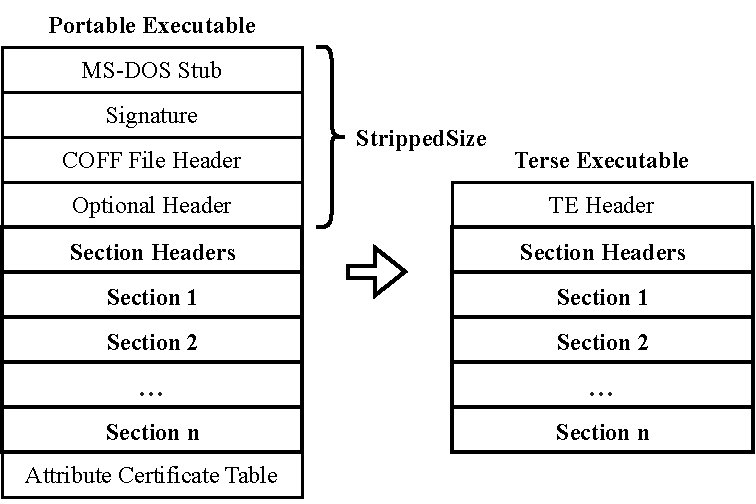
\includegraphics{Figures/PEvsTE.pdf}
  \caption{UEFI PI Terse Executable File Format.}
  \label{fig:pe-vs-te}
  \caption*{The \glsxtrshort{UEFI-PI} specification defines the \glsxtrshort{TE} format in an attempt to reduce the size of \glspl{image-file} compared to their \glsxtrshort{PE} counterparts. This is achieved by removing the \glsxtrshort{PE} \gls{image-file-header} up to the \glsxtrshort{PE} \gls{image-file-section} table and replacing it with a new \glsxtrshort{TE} \gls{image-file-header}. The internal offsets remain unchanged and instead \texttt{StrippedSize} is exposed to the \gls{image-file-loader} so that it can consider the shift in data offsets.}
\end{figure}

The simpler parsing properties of having only a single, simple \gls{image-file-header} are contrasted by the complexity of considering the shift in data offsets and the semantic change to the \gls{image} \gls{address-space}. For \gls{XIP} files, the replacement of the \gls{PE} \gls{image-file-header} also shifts the addresses of all \glspl{image-segment}~\cite{secure-pe}. To account for this, \gls{EDK2}'s \textit{PeiCore} has a workaround to apply the shift to the load address, so that the \gls{image-file-header} is technically misaligned, but the \glspl{image-segment} are correctly aligned~\cite{edk2,secure-pe}. This is especially important when enforcing \gls{memory-permissions} during \glsxtrshort{PEI}.

\subsection{EFI Development Kit II}

The reference implementation of \glsxtrshort{UEFI-PI} and \glsxtrshort{UEFI} named \gls{EDK2} is maintained by the TianoCore community under an open-source licence~\cite{edk2}. Most common \glsxtrshort{UEFI} implementations on the market fork and extend it, such as \glsxtrshort{Microsoft} Project Mu~\cite{mu-basecore}. The \gls{SDK} includes most of the microarchitecture-independent components of the \glsxtrshort{UEFI-PI} and \glsxtrshort{UEFI} specifications, as well as some \gls{ISA}- and microarchitecture-specific industry code~\cite{edk2}. It also implements two fully-featured virtual QEMU~\cite{qemu} platforms, \gls{OVMF} for \glsxtrshort{Intel} architectures, and \gls{ArmVirtQemu} for \glsxtrshort{Arm} architectures.

\section{A Secure PE Loader based on Formal Methods}
\label{sec:formal_pe}

The current \gls{EDK2} \glsxtrshort{PE} \gls{image-file-loader} implementation has been subject to various security and reliability issues over the years~\cite{secure-pe}. Many problems are implementation details that could be fixed evolutionarily, but even the \gls{API} itself is error-prone and unsafe. In response, we proposed a novel implementation with a new \gls{API} that was designed using formal methods. The most critical correctness properties were formally proven using a Frama-C derivative, but late workarounds to support malformed \glsxtrshort{PE} files were not verified. Since its proposal, \gls{AUDK} has completely replaced the old \gls{image-file-loading} with this novel implementation and several parties have expressed interest in improving the security of this particular stack.

Despite its success in improving the security properties of the \gls{EDK2} \gls{image-file-loader} stack, the sheer complexity of the parsing logic and the various build-time configuration options to accommodate malformed real-world \glspl{image-file} introduced a new kind of maintenance burden.

\section{Image File Format Conversion}
\label{sec:img_conv}

Compiler toolchains generally do not support all \gls{image-file} formats available. Also, they are often limited in platform availability. For example, the \glsxtrshort{Apple} Xcode toolchain supports only \glsxtrshort{MACHO} files and is only available for \glsxtrshort{Apple} macOS, while \gls{MSVC} supports only \glsxtrshort{PECOFF} files and is only available on Windows. As such, it is not trivial to generate \glsxtrshort{PE} files on some platforms with their default compiler toolchains. To still support cross-platform and cross-format build environments, several tools to convert between \gls{image-file} formats have been developed.

\subsection{ELF to PE: EDK II GenFw and iPXE elf2efi}
\label{sec:genfw}

For compiler toolchain configurations based on \glsxtrshort{GCC} and sometimes Clang, \gls{EDK2} generates \glsxtrshort{ELF} files in the first step. To convert these into \glsxtrshort{PE} files, the TianoCore tool GenFw is used~\cite{edk2}. It converts \glsxtrshort{ELF} \glspl{image-file-section} to \glsxtrshort{PE} \glspl{image-file-section} while ignoring \glsxtrshort{ELF} \glspl{image-segment}. This is due to the great flexibility offered by \glsxtrshort{ELF} \glspl{image-file-section} by using custom \gls{static-linking} scripts to merge \glsxtrshort{ELF} \glspl{image-file-section} as desired. It does not necessarily perform a strict translation but supports changing the relative offset between \glspl{image-segment} to change the overall \gls{image} \gls{data-alignment} requirement. GenFw also supports other operations, such as extracting \gls{ACPI} tables from \glspl{image-file}. An undocumented detail of the \gls{EDK2} build system is that all \glspl{image-file} are generated as \gls{XIP}, regardless of their phase or purpose.

iPXE follows a similar approach with its separate elf2efi tool~\cite{ipxe}. Unlike GenFw, its sole feature is a best-effort conversion of \glsxtrshort{ELF} to \glsxtrshort{UEFI} \glsxtrshort{PE} \glspl{image-file} without any adjustments.

\subsection{Mach-O to PE: Apple mtoc and Acidanthera ocmtoc}

For Xcode-based compiler toolchains, \gls{EDK2} generates \glsxtrshort{MACHO} files in the first step. These are converted to \glsxtrshort{PE} files using the \glsxtrshort{Apple} tool mtoc, which is part of the \glsxtrshort{Apple} compiler toolset cctools~\cite{apple-cctools}. Unlike TianoCore GenFw with \glsxtrshort{ELF}, mtoc translates the \glsxtrshort{PE} \glspl{image-file-section} from the \glsxtrshort{MACHO} \glspl{image-segment}.

Unfortunately, mtoc has been subject to various bugs that have remained unfixed for years~\cite{ocmtoc}. Recently, \glsxtrshort{Apple} released a version of the parent tool collection cctools which no longer contains mtoc. To the best of our knowledge, it is deprecated, at least for public use.

In response, ocmtoc emerged as a community fork~\cite{ocmtoc}. It also fixed all known issues to date, including the generation of read-write-execute \glspl{image-segment} and malformed debug directories. By default, \glsxtrshort{MACHO} files generated by Xcode do not apply strict read-only \gls{memory-permissions} to immutable data, but merge them into the executable \texttt{\_\_TEXT} \gls{image-segment}~(see \Cref{sec:merge_ro_x}). In coordination with \gls{AUDK}, ocmtoc implemented support for a strictly read-only \gls{image-segment} by moving the corresponding \glspl{image-file-section} to a new \texttt{\_\_DATA\_CONST} \gls{image-segment}~\cite{audk,ocmtoc}. \Glsxtrshort{Apple} took a similar approach for the XNU kernel~\cite{xnu}.

\section{Improving and Testing for Memory Safety}
\label{sec:impr_mem_safety}

The prevalence of memory safety violations and their exploitation has led to various research efforts to reduce both their frequency and their impact. The class of dynamic memory safety violations is often addressed by automatic memory management. This way, freeing memory is usually either handled by \gls{reference-counting} or \gls{garbage-collection}. In the \gls{firmware} domain, this is currently not an option for performance and security reasons. However, in order to build confidence in the safety of our implementation, we have performed extensive safety testing, which we will now discuss.

\subsection{Fuzz Testing}

\Gls{fuzz-testing} is a technique to stress-test a fuzz target with randomly generated inputs. A typical goal is to observe safety violations based on a broad spectrum of inputs. In the context of memory-unsafe languages like \glsxtrshort{C}, this is particularly interesting for discovering memory safety violations~(see \Cref{sec:mem_violations}). However, it is also possible to use it for functionality validation if there is a way to decide~(with great confidence) whether the output is correct.

As most randomly-generated inputs are invalid and thus will likely be rejected quickly, fuzzers evolved to generate inputs in smart ways~\cite{fuzzingbook2023}. One of them is mutation-based \gls{fuzz-testing}, which lets you provide a corpus of valid inputs, which the fuzzer will mutate. This is commonly combined with coverage guidance, preferring mutations that increase some code coverage metric. A proven mutation-based and coverage-guided fuzzer is LLVM libFuzzer, which tightly integrates with the Clang compiler~\cite{libfuzzer}. For coverage guidance, it uses SanitizerCoverage~\cite{sanitizer-cov}.

Beyond arbitrary mutations, sophisticated techniques like grammar \gls{fuzz-testing} surfaced~\cite{fuzzingbook2023}. It allows defining a grammar for inputs to generate valid or otherwise interesting inputs with a much higher probability. Of course, it can still be used to generate invalid inputs. With probabilistic grammar \gls{fuzz-testing}, the probability of getting different kinds of input can be influenced.

Finally, especially relevant for mutation-based \gls{fuzz-testing}, there are new approaches to combine it with symbolic execution to seed the corpus~\cite{10.1145/3183440.3183494,9394032}.

\subsection{Code Sanitizers}

Code sanitizers consist of compiler instrumentation and sometimes shared libraries that can embed various checks to detect erroneous or suspicious behaviour. Two prominent examples are LLVM AddressSanitizer~(ASan) and UndefinedBehaviorSanitizer~(UBSan)~\cite{asan,asan-paper,ubsan}. The former can detect memory exploits and misaligned memory accesses, among other things. The latter detects undefined behaviour in the sense of \glsxtrshort{C}. Both can be combined with \gls{fuzz-testing} to perform basic empirical code safety testing. However, while this is a good way to increase confidence in the implementation, testing can never provide definitive guarantees. For memory-unsafe languages, the only way to derive them is through formal methods, which we will discuss next.

\subsection{Formal Verification}
\label{sec:verification}

Formal verification is a field of techniques for rigorously reasoning about the correctness of algorithms using mathematical methods. The most prominent tools in this area are proof assistants, such as Isabelle/HOL~\cite{isabelle} or Coq~\cite{coq}. While the former relies on classical logic, the latter is limited to intuitionistic logic, at least out of the box. Intuitionistic logic is the basis of the Curry-Howard Correspondence, which defines the isomorphisms commonly known as proofs-as-programs and propositions-as-types~\cite{sorensen2006lectures}. This allows programs to be generated from constructive mathematical proofs. One such product is the optimizing \glsxtrshort{C} compiler CompCert, which has been formally verified using Coq~\cite{compcert}.

However, for various reasons such as code optimizations, tools have emerged to verify software written in traditional programming languages. One such tool is Frama-C~\cite{frama-c}, which is used in safety-critical industries, such as in aviation by Airbus~\cite{cuoq:hal-02263407}. It allows the verification of \glsxtrshort{C} programs for safety properties, such as memory safety, but also for functional properties, which can be provided as formal specifications using \gls{ACSL}~\cite{acsl}.

Formal methods are the only way to guarantee properties such as memory safety for languages without memory safety semantics. However, they are only used in safety- and security-critical scenarios because of their steep learning curve and the enormous effort~(and thus cost) of formalizing and verifying the entire codebase. Sometimes verification covers only a critical subset of a software product. For Coq, the so-called kernel acts as a trusted core~\cite{coq}. It is the only point of failure for the proof assistant. All tactics rely on the kernel to check their output, which are terms in a common proof language. If a tactic produces incorrect output, it may produce false negatives, but never false positives.

\section{The Rust Programming Language}
\label{sec:rust}

The \glsxtrfull{Rust} aims to be a low-level programming language with strong semantic guarantees from the compiler~\cite{rust-ref}. Its most interesting design detail is the ownership and borrowing model for memory allocation. It covers both \glspl{call-stack-memory-allocation} and \glspl{dynamic-memory-allocation} and statically proves all memory accesses to be temporally safe. In addition, \glsxtrshort{Rust} dynamically validates memory bounds on access. This rules out all classes of memory safety violations and guarantees that the code is memory-safe. However, this model is limited and some memory-safe code cannot be expressed with it, such as doubly-linked lists. To still support such use cases, \glsxtrshort{Rust} supports unsafe code, which provides no more guarantees than other languages such as \glsxtrshort{C}. Another related safety feature is the detection of integer overflows, which can sometimes be abused to cause buffer overflows, or, more generally, out-of-bounds accesses.

\subsection{The Borrow Checker and Temporal Memory Safety}

\glsxtrshort{Rust} uses variable bindings, identified by a variable name, to reference allocated memory~\cite{rust-ref}. When the binding goes out of scope, it automatically frees the corresponding memory, much like automatic variables work in \glsxtrshort{C}. However, unlike \glsxtrshort{C}, the safety of this automatic memory management is statically proven. This requires that the binding is authoritative over the lifetime of the memory, i.e. the binding owns the memory. To allow other places in the code to still access the data, but not in a way that can introduce race conditions or dangling references, \glsxtrshort{Rust} introduced the concept of borrowing.

Borrowing can create both immutable and mutable references to memory. Code can create either an arbitrary number of immutable references or exactly one mutable reference. This works in the same way as a \gls{readers-writer-lock} and provides the same guarantees. Not only explicit reference creation takes advantage of this, but iterators also provide only immutable references, preventing iterator invalidation. Since references cannot semantically outlive their resource, \gls{use-after-free} is completely mitigated. Finally, since references are only borrowed and never owned by two locations, there can be no reference cycles, which completely mitigates memory leaks.

There have been attempts to introduce \glsxtrshort{Rust} ownership and borrowing in C++. However, the researchers concluded that the C++ type system did not allow for this~\cite{cpp-borrowing-trouble}.

\subsection{Rust in Linux}
\label{sec:rust-linux}

In 2021, a \gls{RFC} was posted to the Linux kernel mailing list to discuss the addition of \glsxtrshort{Rust} as an official programming language for the Linux kernel~\cite{linux-rust}. However, unlike \gls{user-space} applications, low-level code for \gls{firmware} and operating system kernels has unique requirements. First, they may not provide a full-featured standard library for performance, efficiency, or security reasons. Second, critical interruptions of the control flow~(e.g. exceptions and panics) are unacceptable, because there is no reasonable way to recover from them. This fundamentally deviates from the design of modern programming languages, including \glsxtrshort{Rust}. In order to meet the needs of the kernel, custom solutions and paradigms that are much closer to the traditional design of \glsxtrshort{C} programming have been discussed. Finally, in 2022, the initial \glsxtrshort{Rust} infrastructure landed in the Linux kernel tree~\cite{linux-rust-git}.

\subsection{Formal Verification and RustBelt}

Because of its strict semantics, \glsxtrshort{Rust} can provide some guarantees at build-time that previously could only be established by formal verification~(see \Cref{sec:verification}). For five years, the \gls{MPI-SWS} has researched the development of formal foundations for the \glsxtrshort{Rust} language as part of `RustBelt', including compiler verification similar to CompCert~\cite{rustbelt}. Earlier this year, the official \glsxtrshort{Rust} types team was formed to pursue a formalization of the type system~\cite{rust-types-team}. If successful, much of the burden of the formal verification of safety properties could be shifted from the individual project using \glsxtrshort{Rust} to the \glsxtrshort{Rust} compiler itself.

\chapter{Requirements for a UEFI Executable File Format}
\label{chap:uefi_exec_reqs}

In this chapter, we will perform requirements engineering for the proposal of a new \gls{executable-file} format for \glsxtrshort{UEFI} \gls{firmware}. \Cref{sec:mem_sec} provides insight into various techniques for improving memory security, some of which have been incorporated into the \glsxtrshort{UEFI} reference implementation \glsxtrshort{EDK2}. Then, \Cref{sec:uefi} gives a broad overview of the related \glsxtrshort{UEFI} designs and technologies. Finally, \Cref{sec:uefi_exec} details the requirements of \glsxtrshort{UEFI} for \gls{image-file} formats and supporting code.

\section{Memory Security}
\label{sec:mem_sec}

In response to the exploitation of memory safety violations, \glsxtrshort{CPU} architectures, operating systems, and \gls{firmware} implementations have developed a variety of security approaches~\cite{10.1007/978-3-642-33338-5_5}. These do not address or fix the vulnerabilities themselves but aim to dramatically reduce their impact and the practicality of exploitation. We will now look at some of the more common techniques.

\subsection{Memory Privileges}
\label{sec:mem_privileges}

\Gls{virtual-memory} also allows the maintenance and isolation of multiple \glspl{address-space}. This is particularly useful for isolating \gls{user-space} processes and restricting access to the \gls{kernel-space} \gls{address-space} via \gls{memory-privilege}. In general, there is one \gls{page-table} per \gls{user-space} process, which is shared with the \gls{kernel-space}. So, the \gls{kernel-space} memory is part of the \gls{user-space} \gls{address-space}, but not accessible to the corresponding \gls{user-space} process due to \glspl{memory-privilege} isolation. However, for \gls{side-channel}-related security reasons~\cite{meltdown,kaiser}, some operating system configurations separate the \glspl{page-table} for \gls{kernel-space} and \gls{user-space} to map only the \gls{kernel-space} memory required to bootstrap any \gls{syscall}. In the Linux kernel, this is implemented by a feature called \gls{PTI}~\cite{pti}. To strengthen the isolation in the other direction, \glsxtrshort{Intel} introduced \gls{SMEP} and \gls{SMAP}, which restrict the execution of and memory accesses to \gls{user-space} memory from \gls{kernel-space} unless explicitly requested~\cite{ia32}.

To address the performance penalty of the \gls{PTI} approach and to simplify the implementation, \glsxtrshort{Intel} introduced \gls{LASS}~\cite{ia32-ext}. Unlike existing related solutions such as \gls{SMEP}, \gls{SMAP}, and \gls{PTI}, \gls{LASS} does not rely on \gls{page-table} information and therefore can be used without a \gls{page-table} walk. This is a new approach to mitigating timing-based \gls{side-channel} attacks since deciding whether the address belongs to the \gls{kernel-space} can easily be done in constant time.

\subsection{Memory Permissions}
\label{sec:mem_perms}

\Gls{virtual-memory} management includes not only \gls{address-space} mappings and \glspl{memory-privilege}, but also \gls{memory-permissions}. While \gls{memory-privilege} defines which \glsxtrshort{CPU} mode can perform operations in general, \gls{memory-permissions} define which operations can be performed. The typical operations that can be restricted by \gls{memory-permissions} are reading, writing, and executing memory. Most processors have restrictions on possible combinations~\cite{ia32}. However, historically unconventional \gls{memory-permissions} combinations such as execute-only are supported by some.

For security reasons, \gls{memory-permissions} should generally be configured as tightly as possible. In particular, a non-executable \gls{call-stack} is one of the basic defences against \gls{call-stack-smashing}~(see \Cref{sec:mem_exploits}). However, it is important to note that \gls{page-table} changes can lead to performance degradation for many reasons, such as the need to flush \gls{TLB} caches. Also, \gls{memory-permissions} can only be applied on the level of \glspl{memory-page}, so tightening \gls{memory-permissions} may increase the overall memory requirements. Therefore, deciding the best configuration for each use case requires careful analysis.

\subsection{Mutual Exclusion of Writing and Executing~(W\^{}X)}
\label{sec:mem_wxorx}

\Gls{w-xor-x} is a paradigm in memory security that memory should never be writable and executable at the same time. This prevents so-called self-modifying code, which can be used to exploit vulnerable applications~(often privileged) and bypass security measures such as \glspl{digital-signature} by modifying the code only after it has been authenticated~(see \Cref{sec:mem_exploits}). It also implies a non-executable \gls{call-stack}, as it is writable by nature.

However, there are also legitimate use cases for \glspl{memory-page} that are both writable and executable, such as \gls{JIT}. In response, there have been novel approaches to introducing \gls{w-xor-x} into \gls{JIT} workloads. For example, \glsxtrshort{Apple} silicon provides efficient and thread-specific toggling between being writable and being executable, rather than having to modify the \gls{page-table}~\cite{as-sec}. This avoids some of the penalties associated with typical \gls{memory-permissions} changes.

\subsection{Control Flow Security}

Another attempt to mitigate \glspl{call-stack-overflow} is the use of \glspl{call-stack-canary}~\cite{10.1007/978-3-642-33338-5_5}. Typically, on entering the subroutine, it generates a pseudo-random value and stores it near the \gls{return-address} on the current \gls{call-stack-frame}. Before returning, the subroutine compares the \gls{call-stack-canary} with the original value from a safe location, usually a processor register, to see if it has changed. If the values do not match, a \gls{call-stack-overflow} has occurred and the program terminates to prevent exploitation. However, an obvious shortcoming of this approach is that it does not catch indirect \gls{call-stack} corruptions that leave the \gls{call-stack-canary} intact.

To address these shortcomings, sophisticated \gls{FCFI} and \glspl{shadow-call-stack} have been implemented by \glspl{CPU}~\cite{ia32,arm-isa}, operating systems~\cite{linux-arm-bti}, and \glsxtrshort{UEFI} firmware implementations~\cite{uefi-spec,edk2}. \Gls{FCFI} is implemented in hardware and, when enabled, the compiler marks all jump targets with a special instruction. If the \glsxtrshort{CPU} has \gls{FCFI} enabled, e.g. \gls{BTI}~\cite{arm-isa} or \gls{IBT}~\cite{ia32}, and a jump to an address without such an instruction occurs, the \glsxtrshort{CPU} throws an exception and the operating system may terminate the offending program. This severely limits the candidate pool for \glspl{code-gadget}.

\Glspl{shadow-call-stack} can be implemented either in software, e.g. Clang ShadowCallStack~\cite{clang-csc}, or in hardware, e.g. \glsxtrshort{Intel} \gls{CET}~\cite{ia32}. Their purpose is to keep track of the history of the \glspl{return-address} in a safe place so that the value in the \gls{call-stack-frame} can be verified as authentic. Unlike \glspl{call-stack-canary}, this also detects indirect \gls{call-stack} corruption.

\subsection{Address Space Layout Randomization}
\label{sec:aslr}

Another technique to make \glspl{code-gadget} harder to find is to randomize their locations~\cite{10.1007/978-3-642-33338-5_5,ms-aslr}. \Gls{ASLR} pseudo-randomizes the \glspl{image-base-address} of all \glspl{shared-library}~(called \gls{PIC}) and \glspl{executable-file}~(called \glspl{PIE}), the \gls{heap-memory}, and the \gls{call-stack} memory addresses. Unlike Windows~\cite{ms-dll-base-addr}, Linux and macOS even pseudo-randomize the \gls{image-base-address} of \glspl{shared-library} per process rather than globally.

As attacks against \gls{ASLR} have surfaced, additional hardening, such as Function Granular \gls{KASLR} that even randomizes function addresses within an \gls{image}, was deployed~\cite{fgkaslr}.

\subsection{Allocator Hardening against UAF Type Confusion}

A relatively recent development in memory security is the hardening of \gls{dynamic-memory-allocation} against \gls{use-after-free} type confusion attacks. In this context, this does not refer to confusing the type of a live object, but between a previously freed object and a live object that now owns that memory. For its XNU kernel, \glsxtrshort{Apple} has implemented best-effort protection against confusing pointer and non-pointer data between reallocations~\cite{apple-mem-alloc}. This is achieved by type buckets, which are calculated at build-time. The build system chooses the buckets so that there is no overlap between pointers and non-pointer data across all its types. Once a \gls{virtual-memory} address has been allocated to a particular bucket, it can never be reallocated to an object from another bucket. This effectively prevents \gls{use-after-free} vulnerabilities from being exploited to interpret arbitrary data as an address. While this does not mitigate the \gls{use-after-free} vulnerabilities themselves, it can mitigate their exploitability~\cite{apple-mem-alloc-ex}.

\subsection{Takeaways from Memory Safety and Memory Security}

Memory exploits are not explicitly within the scope of this work. We will discuss \gls{ASLR} and \gls{FCFI} in the context of \glsxtrshort{UEFI} and \gls{image-file} next, but our contribution cannot help harden memory security. The key takeaway from exploring the field of memory security is that, while it is crucial to provide defence-in-depth against potentially stealthy and critical software exploits, it cannot give us sufficient guarantees, no matter how sophisticated it becomes. On the other hand, if we managed to guarantee memory safety, most techniques that harden memory exploits would not be required. As parsing \glspl{executable-file} requires handling a lot of potentially malicious data, with the ultimate goal to execute it, memory safety is of utmost importance. Still, memory security should be employed or at least not explicitly hindered where possible.

\subsection{Memory Security in Image File Formats and UEFI}

The \glsxtrshort{UEFI} specification and \gls{EDK2} include some security features discussed above~\cite{uefi-spec,edk2,edk2-memory-safety}. \Gls{memory-permissions}, \glspl{call-stack-canary}, and \gls{FCFI} are supported by \gls{EDK2}, while \gls{ASLR} is still in the proof-of-concept phase~\cite{edk2-memory-safety}. Unlike operating systems, \glsxtrshort{UEFI} must guarantee that certain memory does not move across resets, which severely limits the potential of \gls{ASLR}. While the most common examples are resuming from sleep states, \glsxtrshort{EDK2} supports memory type bins that are iteratively tuned in size~\cite{edk2}. The \gls{memory-page} and pool allocators will try to fit all \glspl{dynamic-memory-allocation} into these bins first, before resorting to other areas of memory. The design of this feature fundamentally contradicts the idea of \gls{ASLR}, which also needs to be addressed in the future.

However, while \gls{EDK2} theoretically supports tight \gls{memory-permissions}, some operating systems and \glspl{os-loader} still assume data allocations to be executable or request read-write-execute \gls{memory-permissions}~\cite{grub-nx-bug,linux-wxorx}. Unfortunately, \gls{w-xor-x} is not yet widely supported due to implementation details that rely on shared memory between code and data~\cite{edk2-wxorx}. For \gls{image-file-loading} in particular, \gls{EDK2} also does not support read-only memory, and instead silently makes it writable~\cite{edk2-granular-pe}.

In the context of \glspl{image-file}, \gls{FCFI} only affects code generation, so it is independent of the \gls{image-file} format. However, each format requires some way of signalling that \gls{FCFI} is supported by the \gls{image-file}~\cite{pe-format}.

\section{The Unified Extensible Firmware Interface}
\label{sec:uefi}

Modern computer platforms require complex initialization to function as expected~\cite{pi-spec}. This can include tasks such as updating the \glsxtrshort{CPU} \gls{microcode}, initializing the main memory, or booting the operating system. In the past, there were mostly handled by proprietary and closed \gls{firmware} implementations, such as the \gls{BIOS} for \glsxtrshort{Intel} architecture \glspl{CPU}~\cite{bios-spec}. With increasing complexity and the need for interoperability, the industry moved to a new modular and extensible alternative, known as the \glsxtrfull{UEFI}~\cite{uefi-spec}. It has since become the supported boot specification for the \glsxtrshort{Microsoft} Windows operating system~\cite{win10-hwreq}. Companies such as \glsxtrshort{Qualcomm} also use it for various mobile device platforms, such as \gls{SoC} products used in Android phones and tablets~\cite{qc-uefi}.

Most \glsxtrshort{UEFI} implementations conform to both the \glsxtrfull{UEFI-PI}~\cite{pi-spec} and the \glsxtrshort{UEFI}~\cite{uefi-spec} specifications. While the former deals with external compatibilities, such as providing services and specifications for applications and \glspl{os-loader}, the latter deals with internal compatibilities, such as providing services useful for hardware initialization. Both are owned and published by the \glsxtrshort{UEFI} Forum.

The specifications specify the \glsxtrshort{PE} format for \glsxtrshort{UEFI-PI} and \glsxtrshort{UEFI} modules of all kinds~\cite{pi-spec,uefi-spec}. \Glsxtrshort{SEC} and \glsxtrshort{PEI} modules can alternatively be \glsxtrshort{TE} \gls{executable-file}. Our contribution is to replace this dependency with an optional alternative \gls{executable-file} format. To get an idea of the requirements for such an alternative, let us first discuss the basic workings of \glsxtrshort{UEFI}.

\subsection{UEFI PI Phases of Execution}
\label{sec:pi-phases}

The \glsxtrshort{UEFI-PI} specification describes several phases of execution~(see \Cref{fig:uefi_phases})~\cite{pi-spec}. This design follows the multi-phase process of hardware initialization used by different types of platforms. Some phases essentially extend \glsxtrshort{UEFI} concepts~\cite{pi-spec,uefi-spec}. For example, \glsxtrshort{UEFI-PI} \glsxtrshort{BDS} implements the \gls{UEFI-Boot-Manager}.

\begin{figure}[htb]
  \centering
  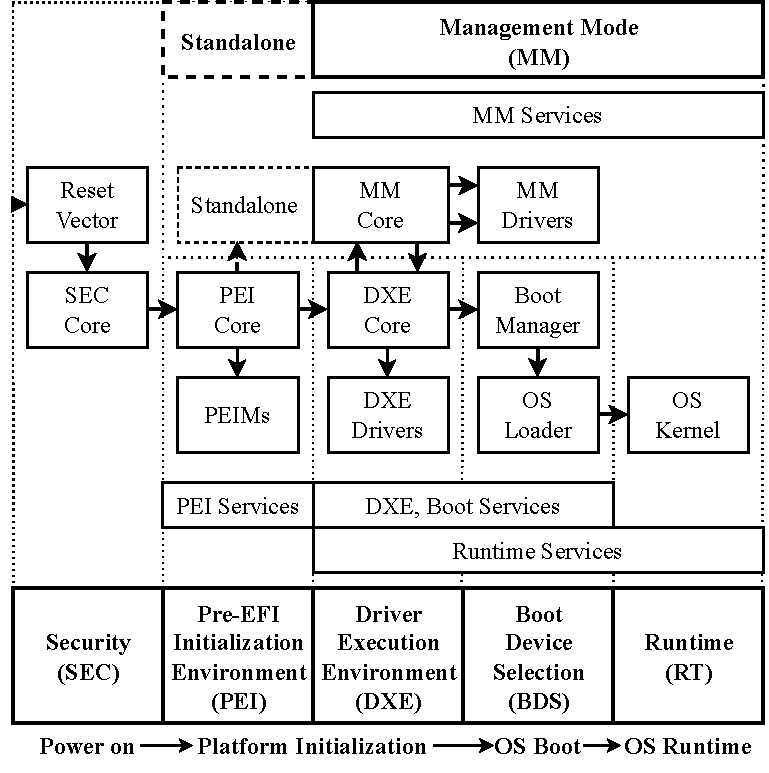
\includegraphics{Figures/UEFIPIPhases.pdf}
  \caption{UEFI PI Phases of Execution.}
  \label{fig:uefi_phases}
  \caption*{The \glsxtrshort{UEFI-PI} phases of execution and the corresponding \glspl{module-dispatcher} and services. For more information on the phases, see \Cref{sec:pi-phases}.}
\end{figure}

\subsubsection{Security~(SEC)}

The \glsxtrfull{SEC} phase is the first phase to be invoked, for example by power events such as starting or rebooting the device~\cite{pi-spec}. In general, its purpose is to prepare the environment for the execution of generic \glsxtrshort{C} code. This may include updating the \glsxtrshort{CPU} \gls{microcode} or checking the health of the \glsxtrshort{CPU}. The most important task however is to set up a temporary memory that can serve as a \gls{call-stack}. Traditionally, this is done using a technique called \gls{CAR}. \Glsxtrshort{Intel} platforms implement this using the \glsxtrfull{NEM}, which disables cache line eviction on cache misses, thus guaranteeing the persistence of stored data. Due to its nature as the first software invoked, it serves as the \gls{SRoT} of the \glsxtrshort{UEFI-PI} \gls{firmware} model. Once it completed all its initialization tasks, \glsxtrshort{SEC} invokes the \glsxtrshort{PEI} phase.

\subsubsection{Pre-EFI Initialization~(PEI)}

The \glsxtrfull{PEI} phase is the second phase to be invoked, usually immediately after the \glsxtrshort{SEC} phase~\cite{pi-spec}. In the past, its sole purpose was to initialize the permanent main memory in a simplified environment. However, with the introduction of features such as platform recovery~(e.g. in case a \gls{firmware} update fails), this is not strictly true with the current generation of \glsxtrshort{UEFI-PI} implementations. Some modern platforms, such as the \glsxtrshort{AMD} Ryzen family of \glspl{CPU}, no longer perform initialization of the main memory as part of the platform \gls{firmware} and have instead moved it to less open hardware, such as the \glsxtrshort{AMD} \gls{PSP}~\cite{ryzen-ram-init}.

When resuming from platform sleep, \glsxtrshort{PEI} executes so-called S3 boot scripts to restore the platform state destroyed by the platform sleep state invocation~\cite{pi-spec}. These S3 boot scripts can be modified by \glsxtrshort{PEI} or subsequent phases to preserve their platform initialization operations. Consequently, \glsxtrshort{UEFI-PI} skips subsequent phases when resuming from platform sleep.

\subsubsection{Driver Execution Environment~(DXE)}

The \glsxtrfull{DXE} phase is the third phase to be invoked~\cite{pi-spec}. However, it can be skipped for certain platform boot paths, such as resuming from platform sleep. Its primary purpose is to initialize the remaining hardware which was not yet initialized by the \glsxtrshort{PEI} phase and to establish platform security. Initialization can include the platform chipset, PCIe devices, storage interfaces, and more. \Glsxtrshort{DXE} establishes platform security by locking down \glsxtrshort{MM}~(e.g. no new \glsxtrshort{MM} communication buffers can be allocated after it has finished) and optionally write-protecting the \gls{firmware} storage. It also implements \gls{secure-boot} and \gls{measured-boot} to authenticate Option ROMs and \glspl{os-loader}~(see \Cref{sec:sb_mb}).

\subsubsection{Boot Device Search~(BDS)}

The \glsxtrfull{BDS} phase is the fourth phase to be invoked~\cite{pi-spec}, usually just after \glsxtrshort{DXE}. It may not be reached if the platform is reset early for any reason~(e.g. when applying a \gls{firmware} update). Its primary purpose is to locate and pass control to bootable code, such as an \gls{os-loader}.

However, as many machines require a degree of customizability, it can also invoke built-in applications, such as a configuration utility or a boot menu for multiple operating systems, based on user interaction. To enable this, various peripherals such as mice, keyboards, video outputs, and the like~(commonly referred to as \glspl{HID}) need to be initialized. This is done by the \gls{UEFI-Boot-Manager}, which is the abstract concept of \glsxtrshort{BDS} outside \glsxtrshort{UEFI-PI}. The \gls{UEFI-Driver-Model} allows drivers to probe devices and attach to them if they are supported. User input, such as keyboard hotkeys, can then trigger various actions, such as invoking the boot menu or rebooting the platform.

\subsubsection{Transient System Load~(TSL), Runtime~(RT), and Afterlife~(AL)}

The \glsxtrfull{TSL} phase is more of a transition~\cite{pi-spec}. It begins with the invocation of the \gls{os-loader} and ends when the operating system has finished transitioning \glsxtrshort{UEFI} to the \glsxtrfull{RT} phase, by providing \gls{kernel-space} address mappings for the \glsxtrshort{UEFI} \glsxtrshort{RT} data. Unlike the other phases, \glsxtrshort{RT} does not control the system itself but is an aid to the operating system, which can call so-called \glsxtrshort{UEFI} Runtime Services on demand. The idea is to abstract hardware-dependent functionality with \glsxtrshort{C} code that can be called in the \gls{kernel-space} context. The \glsxtrfull{AL} phase is also not strictly a phase either, but the process of shutting down the platform.

\subsubsection{Traditional and Standalone Management Mode~(MM)}

The \glsxtrfull{MM} phase is not strictly a phase like the others, but once it is set up, it is entered on demand~\cite{pi-spec}. It can either be set up during the \glsxtrshort{DXE} phase and access all the services and \glspl{uefi-protocol} it provides, known as \gls{TMM}. Or it can be set up during the \glsxtrshort{PEI} phase and not access any external services on its own, known as \gls{StMM}. Derived from the \glsxtrshort{Intel} System Management Mode, its primary purpose was to handle power management functions during the operating system runtime. However, with modern \glsxtrshort{Intel} and \glsxtrshort{AMD} chips, this functionality has been moved to the \glsxtrshort{CPU} itself. \Glsxtrshort{MM} remained as a high-privilege mode used for security isolation. For example, before loading third-party code, modern \glsxtrshort{Intel} and \glsxtrshort{AMD} platforms typically restrict write operations to the \gls{firmware} \gls{SPI} to \glsxtrshort{MM}, for security reasons. To still be able to write \gls{NVRAM} variables at runtime, a \glsxtrshort{RT} driver sends the request to a \glsxtrshort{MM} driver, which then writes the variable if allowed.

\subsection{Module Dispatchers and the Image File Loader}

\Glsxtrshort{UEFI-PI} \glspl{module-dispatcher} handle the scheduling of modules in a correct order~\cite{pi-spec}. They process \glspl{FVg} and repeatedly start all modules that have all their dependencies met. Dependencies, which can be \glspl{PPI} or \glspl{uefi-protocol}, are described by the \gls{depex} section for \glsxtrshort{UEFI-PI} \glspl{PEIM} and \glsxtrshort{DXE} drivers. As \glspl{PPI} and \glspl{uefi-protocol} can be installed at any point in time, the loading order of the modules can only be determined at runtime. To load and start these modules, the \glspl{module-dispatcher} uses a \glsxtrshort{TE} and \glsxtrshort{PE} \gls{image-file-loader}. Strictly speaking, the \glspl{module-dispatcher} themselves only process \glspl{image-file} from the \gls{firmware} storage, which are authentic if the \glspl{FVg} are all digitally signed. However, the \glsxtrshort{BDS} phase may load \glsxtrshort{UEFI} drivers, applications, and \glspl{os-loader} from untrusted storage, which pass through the very same infrastructure. These \glspl{image} are not subject to the same intrinsic trust and must be handled with great care to avoid exposing exploitable behaviour to attackers.

In addition to ensuring memory-safe parsing code, trust can be established by authenticating that the \gls{image-file} is trusted by a platform authority. Next, we will discuss \glspl{chain-of-trust} and how they can be used to authenticate the entire platform boot process.

\begin{figure}[htb]
  \centering
  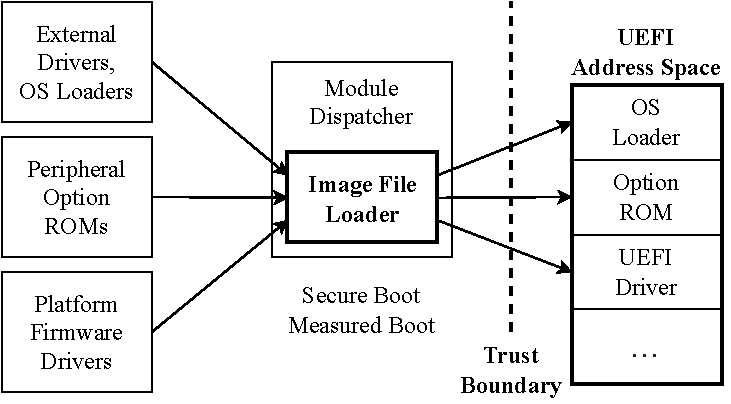
\includegraphics{Figures/UefiLoader.pdf}
  \caption{Role of the Image File Loader in UEFI PI and UEFI.}
  \caption*{The \gls{image-file-loader} is a central component of the \glspl{module-dispatcher} for \glsxtrshort{PEI}, \glsxtrshort{DXE}, and \glsxtrshort{MM}. While \glsxtrshort{PEI} and \glsxtrshort{MM} deal almost exclusively with platform drivers, \glsxtrshort{DXE} traditionally loads Option ROMs and \glspl{os-loader} from untrusted media. As such, it must be resilient to memory safety violations caused by maliciously-created \glspl{image-file}. The same applies to \gls{image} authentication, as all \gls{image} run with critical privileges.}
\end{figure}

\subsection{Roots of Trust and Chains of Trust}

\Glspl{chain-of-trust} are the foundation of authority-based security designs. They start with an axiomatically trusted entity, the \gls{RoTg}, which could be a product owner, for example. In user-space software designs, this can be implemented with a \gls{root-digital-certificate} known to belong to the product owner, while in hardware designs it is typically a security chip that the product owner may have developed or validated. From there, the \gls{RoTg} authenticates the next entity in the chain. Continuing with the hardware \gls{chain-of-trust}, this could be its own \gls{firmware}. Further down the line, there are multiple layers of components that may span across multiple supply chains and involve multiple product vendors. For example, the security chip \gls{firmware} may authenticate a more general platform \gls{firmware}, and the platform \gls{firmware} may load a hardware driver provided by a third party. When the platform \gls{firmware} authenticates this driver, it is represented as another link in the \gls{chain-of-trust}. The general idea is that trust is transitive, so if the platform \gls{firmware} trusts the driver, and the \gls{RoTg} trusts the platform \gls{firmware}, then the platform trusts the driver.

However, trust is not necessarily a binary property. For example, an entity may only be trusted only with certain platform resources and privileges. Transitive trust must never extend the scope of trust. For example, \glspl{CAg} can never sign \glspl{digital-certificate} or data outside their scope. By limiting their privileges, the impact of abuse and exploitation is limited, which is why links towards the root are privileged and well protected~(e.g. protected by \glspl{HSM} and physical security), while links towards the leaf are a lot more limited but accessible.

To reduce the risk of unnoticed exploitation, \glspl{digital-certificate} have a limited validity timeframe and must be renewed before expiring. Leaf \glspl{digital-certificate} are usually only valid for a few months or around a year, while a \gls{root-digital-certificate} may be valid for multiple decades. The higher the chain a link is, the harder it is to renew. In the event of a theoretical security vulnerability or exploitation, one can revoke trust in any link in the chain. This is also not necessarily binary --- optionally, with a timestamp of revocation, data signed prior to revocation can still be trusted.

Besides a plain \gls{chain-of-trust}, \glspl{digital-signature} and \glspl{trusted-timestamp} can be used to implement more sophisticated security features. For example, with personalized~(in the sense of the target computer) and on-demand signing~(which enables the use of nonces for an interactive update process), soft downgrade protections can be implemented. With a naive approach, after a configurable amount of time, the update server simply stops signing old updates and their \glspl{digital-signature} expire. \Glsxtrshort{Apple} implements a more sophisticated approach that roughly follows the same ideas~\cite{apple-sec}.

Examples of Hardware \glspl{RoTg} are \gls{Intel-ME} and \glsxtrshort{Apple} T2~\cite{apple-sec,uefi-secure-boot}. Next, we will discuss how \gls{verified-boot} uses them to authenticate the entire platform \gls{firmware} using a \gls{chain-of-trust}.

\subsection{Verified Boot and Intel Boot Guard}

\Gls{verified-boot} applies establishes a \gls{chain-of-trust} for the platform \gls{firmware} to authenticate the entire boot process~\cite{uefi-secure-boot}. \Gls{Intel-Boot-Guard} is one of the technologies that make this possible~(see \Cref{fig:boot-guard}). With it, \gls{Intel-ME} acts as a \gls{HRoT}, which verifies the \gls{IBB} of the platform \gls{firmware}. As the \gls{reset-vector} resides on secondary \gls{SPI} memory and \glsxtrshort{Intel} platforms still require a lot of code to initialize the main memory, the said \gls{IBB} generally covers all pre-memory \glspl{FVg}. To mitigate \gls{TOC-TOU} attacks when shadowing the post-memory \glspl{FVg} into the main memory, they are covered by a separate \gls{OBB}, which in practice is more of a logical collection of \glspl{FVg}. The \gls{firmware} exposes authenticated \glspl{cryptographic-hash} for them, which allows their authentication in software by \glsxtrshort{PEI} after they have been shadowed~(\gls{EDK2} \textit{FvReportPei}). Due to the generally low speed of \gls{SPI} memory, authenticating after shadowing improves the boot performance.

\begin{figure}[htb]
  \centering
  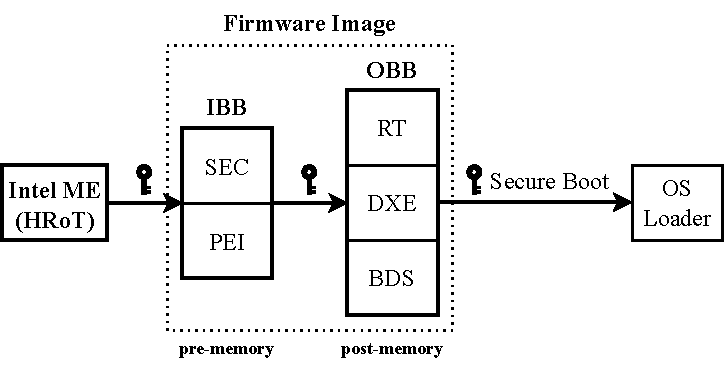
\includegraphics{Figures/BGRoT.pdf}
  \caption{Verified Boot based Intel Boot Guard.}
  \label{fig:boot-guard}
  \caption*{\Gls{Intel-Boot-Guard} uses \gls{Intel-ME} as the \gls{HRoT} for platform \gls{firmware} authentication. It authenticates the \gls{IBB}, which contains all the code required to run before initializing the system memory. The \gls{IBB} is then responsible for authenticating the \gls{OBB} once it has been shadowed into system memory. If important data resides outside both blocks or if anything from the \gls{OBB} is authenticated before shadowing, the scheme may not be secure.}
\end{figure}

\Glsxtrshort{Apple} moved the entire \gls{firmware} image and authentication logic to their \gls{HRoT} \glsxtrshort{Apple} T2~(see \Cref{fig:t2_boot}). This will mitigate all the issues discussed above.

\begin{figure}[htb]
  \centering
  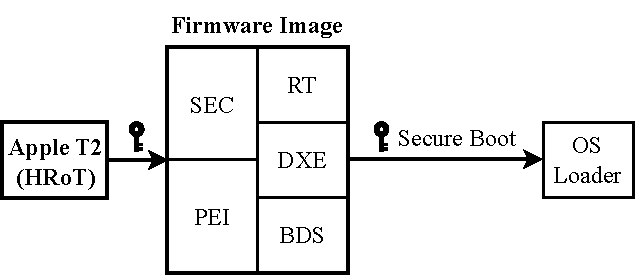
\includegraphics{Figures/T2RoT.pdf}
  \caption{Verified Boot based on Apple T2.}
  \label{fig:t2_boot}
  \caption*{Similar to \Cref{fig:boot-guard}. However, unlike \gls{Intel-ME}, \glsxtrshort{Apple} T2 authenticates the entire \gls{firmware} image as a whole before powering on the main processor. This means that there can be no data that is not authenticated. Since the \gls{HRoT} itself carries the \gls{firmware} image, there can be no \gls{TOC-TOU} attacks related to shadowing to system memory.}
\end{figure}

\subsection{Secure Boot and Measured Boot}
\label{sec:sb_mb}

The \glsxtrshort{UEFI} specification has not only advanced the operating system boot process and the maintainability of \gls{firmware} implementations, but it also introduced several new security features.

One of them is \gls{secure-boot}, an umbrella term for a software stack in \glsxtrshort{UEFI} \gls{firmware} implementations to cryptographically authenticate \glspl{image-file} using \glspl{digital-signature}. In the consumer market, this means that devices are generally shipping with the `\glsxtrshort{Microsoft} Windows Production \glsxtrshort{CA} 2011' certification authority pre-installed~\cite{ms-sbkey}. \Glsxtrshort{Microsoft} also provides the `\glsxtrshort{Microsoft} 3rd Party \glsxtrshort{UEFI} \glsxtrshort{CA}' certificate authority to third parties to centralize the \gls{secure-boot} management, e.g. for the Linux operating systems landscape~\cite{ms-sbkey3rd}. The operating systems by \glsxtrshort{Microsoft} and \glsxtrshort{Apple} expand code authentication into the \gls{user-space}. While Windows only authenticates \glspl{executable-file} and \glspl{shared-library}, those by \glsxtrshort{Apple} generally authenticate the entire system image~\cite{apple-sec}. Recently, a flexible framework to authenticate~(a subset of) the system image independent of the operating system has been showcased~\cite{amaranth}. Most operating systems based on Linux do not have any load-time authentication at all, but the kernel supports dm-verity and fs-verity, which are leveraged by Android and ChromeOS~\cite{linux}.

Another security feature specified by the \glsxtrshort{UEFI} specification is \gls{measured-boot}, a currently enterprise-oriented scheme to collect critical information about the boot environment and send it to a remote attestation entity, usually a server. This information may include hardware and \gls{firmware} configuration or loaded drivers, depending on the platform policy.

\subsection{Human Interface Infrastructure~(HII)}

\Glsxtrshort{UEFI} drivers and applications may expose and consume \glsxtrfull{UEFI-HII} concepts. They are the foundation of user input and output in \glsxtrshort{UEFI}, such as fonts, localization, and graphical interfaces as a whole. The \glsxtrshort{UEFI-HII} database aggregates resources from so-called \glsxtrshort{UEFI-HII} packages. Conventionally, the \glsxtrshort{PE} resource directory carries a \glsxtrshort{UEFI-HII} package list that encodes these. It is then located by the \gls{module-dispatcher} at load-time and installed as an \glsxtrshort{UEFI} protocol on the module's \glsxtrshort{UEFI} handle~\cite{uefi-spec}. \Gls{EDK2} however also supports exposing \glsxtrshort{UEFI-HII} package data to the module via \glsxtrshort{C} variables, depending on the \lstinline{UEFI_HII_RESOURCE_SECTION} build option~\cite{edk2-module-writers,edk2}.

Outside of modules consuming their own \glsxtrshort{UEFI-HII} packages, the \gls{EDK2} Shell utilizes the separate \glsxtrshort{PE} resource section to extract help strings. This requires the \glsxtrshort{PE} file to be fully loaded, including setting up permissions to execute. Alternatively, the \gls{EDK2} Shell supports bundled help strings and manual files~\cite{edk2}. The overcomplicated parsing logic of the \glsxtrshort{PE} resource directory has been subject to functional defects~\cite{secure-pe}.

\section{UEFI Requirements for Executable Files}
\label{sec:uefi_exec}

Because \glsxtrshort{UEFI} differs from the design of modern operating systems in several ways, it has unusual requirements and use cases for \glspl{image-file}. We will take a look at the most important unique scenarios below.

\subsection{Execute-in-Place, Preloading, and Shadowing}
\label{sec:peim_reqs}

Some platforms do not have any main memory available upon platform reset and instead repurpose dramatically smaller cache memory in order to support things like \gls{call-stack} memory, as required for the execution of \glsxtrshort{C} code~\cite{pi-spec,ISO:2018:III}. \Gls{firmware} developers generally call this \gls{CAR}. As said cache memory is sparse, \glsxtrshort{Intel} platforms running \glsxtrshort{UEFI} \gls{firmware} implementations utilize a technique called \gls{XIP}, which lets the \glsxtrshort{CPU} fetch and execute instructions directly from the \gls{firmware} storage~(generally connected via \gls{SPI})~\cite{pi-spec}. For this, the \glsxtrshort{CPU} maps the \gls{firmware} storage at an address known at build-time~\cite{ia32}. To prevent accidental modification of the \gls{firmware} storage, the \gls{MMIO} mapping is generally read-only. Thus, \gls{XIP} \glspl{image} cannot write to global variables~\gls{EDK2}.

The build tools store \gls{XIP} \glspl{image} `preloaded' so that they can be executed without loading or relocating at run-time~\cite{pi-spec,edk2}. \Gls{image-preloading} in this context refers to performing \gls{image-file-loading} and \gls{image-relocation} to the predetermined \gls{image-base-address} at build-time. This especially implies that the \gls{firmware} storage must hold the entire \gls{image} \gls{address-space} without compression techniques, such as omitting trailing zero values of \glspl{image-segment} as done by \glspl{image-file}.

When main memory has been initialized and is available, important \glspl{PEIM} can be transferred from \gls{CAR} memory to the main memory by a technique called \gls{PEIM-shadowing}~\cite{pi-spec}. This process copies the entire \gls{image} \gls{address-space} from the old to the new memory location and performs \gls{image-relocation}. As the same applies to \gls{call-stack} and \gls{heap-memory}, the \glsxtrshort{PEI} services provide a procedure for pointer conversion every \gls{PEIM} must call on all pointers to such memory.

\subsection{Runtime Image Relocation}

\Gls{runtime-image-relocation}, similar to \gls{PEIM-shadowing}~(see \Cref{sec:peim_reqs}), is used for \glsxtrshort{RT} drivers to support \gls{virtual-memory} mappings decided by the operating system~\cite{pi-spec}. In macOS, this has the side effect of extending \gls{KASLR} to the \glsxtrshort{UEFI} runtime memory, as it is mapped adjacent to the operating system kernel \gls{address-space}~\cite{xnu}.

By the time the \gls{firmware} performs \gls{runtime-image-relocation}, likely all the \glsxtrshort{RT} drivers have already been executed. This means that the targets of \glspl{image-relocation-fixup} may have changed, e.g. by changing global variables that were statically initialized with pointers. There are three ways to handle this situation tolerantly:
\begin{enumerate}
  \item Apply the \glspl{image-relocation-fixup} as usual. This can cause faults if overwriting global variables that were statically initialized with an in-\gls{image} address with an external address~(see \Cref{fig:native_uefi_rt_reloc}). The \glsxtrshort{UEFI} specification does not explicitly describe this as the standardized method, but there is no implication that there should be any workaround~\cite{uefi-spec}.
  \item Apply an \gls{image-relocation-fixup} only if its value is unchanged. This can cause bugs when overwriting global variables that were statically initialized with an in-\gls{image} address with a different in-\gls{image} address and not calling \lstinline|ConvertPointer()|~(see \Cref{fig:real_uefi_rt_reloc}). \Gls{EDK2} and real-world \gls{firmware} took this approach~\cite{edk2}.
  \item Apply an \gls{image-relocation-fixup} only if its value is in the \gls{image} \gls{address-space}. This would work correctly for most cases. However, at least Clang can emit \gls{image-relocation-fixup} values that are not addresses themselves, but offsets to constants that form an address. While we have only been able to observe this for a single driver~(\gls{EDK2}'s \textit{FatPei}~\cite{edk2}) and only for the \glsxtrshort{Intel} 32-bit architecture, this scenario would cause an extremely rare and difficult-to-debug fault. We are not aware of any implementations of this behaviour and have only described it for completeness.
\end{enumerate}

As we can see, all tolerant approaches can lead to unobvious faults and bugs. Intolerant handling, i.e. aborting if an \gls{image-relocation-fixup} value does not match its old value, does not suffer from any of these problems. However, it does limit the expressiveness of \glsxtrshort{RT} driver code, since this constraint may reject valid \glsxtrshort{C} code.

\begin{lstfloat}[htbp]
  \centering
  \begin{lstlisting}[style=c]
uint8_t mRuntimeDatum = 0;
// This emits an image relocation fixup.
char    *mRuntimePtr  = &mRuntimeDatum;

// Change the address of mRuntimePtr to something
// outside the current image before runtime
// relocation.
void PreRuntimeReloc() {
  mRuntimePtr = NULL;
}

// Naive operation performed by the firmware on
// runtime image relocation.
// void AtRuntimeReloc(uintptr_t ImageSlide) {
//   mRuntimePtr += ImageSlide;
// }

// Process mRuntimePtr after runtime image
// relocation.
void PostRuntimeReloc() {
  if (mRuntimePtr != NULL) {
    *mRuntimePtr = 0;
  }
}
  \end{lstlisting}
  \caption{Fault from Naive UEFI Runtime Image Relocation.}
  \label{fig:native_uefi_rt_reloc}
  \caption*{Faulting program assuming naive \glsxtrshort{UEFI} \gls{runtime-image-relocation}. This strictly assumes the \glsxtrshort{UEFI} specification's description of \lstinline|SetVirtualAddressMap()|~\cite{uefi-spec}. As \lstinline|mRuntimePtr| is initialized with the absolute address of a global variable, an \gls{image-relocation-fixup} is emitted for it~(see \Cref{sec:reloc}). Before entering the runtime phase, we set the pointer to \lstinline[style=c]|NULL|. Due to the recorded \gls{image-relocation-fixup} for the previous address, \lstinline[style=c]|NULL| is relocated, and the final value is exactly \lstinline|ImageSlide = NewBase - OldBase|, i.e. a rogue pointer. After the \gls{runtime-image-relocation} has succeeded, we run some code that changes the value of \lstinline|mRuntimePtr| if and only if it is not \lstinline|NULL|, a common way to signal pointer liveness. At this point, we corrupt arbitrary memory, even though the code is semantically correct.}
\end{lstfloat}

\begin{lstfloat}[htbp]
  \centering
  \begin{lstlisting}[style=c]
uint8_t mRuntimeDatum1 = 0;
uint8_t mRuntimeDatum2 = 0;
// This emits an image relocation fixup.
char    *mRuntimePtr   = &mRuntimeDatum1;

// Change the address of mRuntimePtr to something
// else inside the current image before runtime
// relocation.
void PreRuntimeReloc() {
  mRuntimePtr = &mRuntimeDatum2;
}

// Real-world operation performed by the firmware
// on runtime image relocation.
// void AtRuntimeReloc(
//   void      *OrigPtr,
//   uintptr_t ImageSlide
//   ) {
//   if (mRuntimePtr == OrigPtr) {
//     mRuntimePtr += ImageSlide;
//   }
// }

// Process mRuntimePtr after runtime image
// relocation.
void PostRuntimeReloc() {
  mRuntimeDatum2 = *mRuntimePtr;
}
  \end{lstlisting}
  \caption{Bug from Real-World UEFI Runtime Image Relocation.}
  \label{fig:real_uefi_rt_reloc}
  \caption*{Erroneous program assuming real-world \glsxtrshort{UEFI} \gls{runtime-image-relocation}. This bug mirrors the fault from \Cref{fig:native_uefi_rt_reloc}. Real-world \glsxtrshort{UEFI} implementations only relocate values that remain unchanged~\cite{edk2}, which mitigates the previous fault. Before entering the runtime phase, we change \lstinline|mRuntimePtr| to point to \lstinline[style=c]|mRuntimeDatum2|. As its address is different from that of \lstinline[style=c]|mRuntimeDatum1|, the \gls{image-relocation-fixup} is not applied, even though the address is within the \gls{image} \gls{address-space}. After the \gls{runtime-image-relocation} has succeeded, we run some code that should effectively assign \lstinline|mRuntimeDatum2| to itself. However, due to the incorrect address of \lstinline|mRuntimePtr|, we are reading arbitrary memory. One could argue that according to the \glsxtrshort{UEFI} specification, \lstinline|ConvertPointer()| should have been called on \lstinline|mRuntimePtr|, which resolves the bug~\cite{uefi-spec}. However, the vague wording about reapplying of \glspl{image-relocation-fixup} and the correct behaviour for unmodified pointers make the situation ambiguous.}
\end{lstfloat}

\subsection{Mixed-Mode Execution}
\label{sec:mixed-mode}

\Gls{firmware} implementations for 64-bit \glspl{CPU} based on \glsxtrshort{Intel} architecture typically implement mixed-mode execution~\cite{intel-fsp}. The \glsxtrshort{CPU} powers up in $16$-bit mode~\cite{ia32} and \glsxtrshort{SEC} switches it into $32$-bit mode, which is the main operating mode throughout \glsxtrshort{PEI}~\cite{edk2}. Only when transitioning into \glsxtrshort{DXE}, the \glsxtrshort{CPU} finally switches into 64-bit mode. One of the main reasons for mixed-mode execution is the reduced memory requirements of the $32$-bit code~\cite{mixed-mode-1,mixed-mode-2}. While work is underway to move \glsxtrshort{PEI} completely to 64-bit mode~\cite{mixed-mode-1,mixed-mode-2} and future microarchitecture proposals deprecate $16$-bit and 64-bit modes for low-level operation~\cite{x86s}, mixed-mode execution is a strict requirement for the time being. Most importantly, it means that a single \gls{image-file} can carry code targeting multiple \glspl{ISA}, which is particularly relevant for \gls{image-relocation}.

\subsection{Fixed-Address Loading}
\label{sec:fixed-addr}

In stark contrast to \gls{ASLR}, some embedded system designs mandate fixed memory maps. This is a typical consequence of prohibiting the use of \gls{dynamic-memory-allocation} to establish worst-case guarantees for memory usage and allocation times~(see \Cref{sec:heap_mem_alloc}). To achieve this, the build system must, among other things, statically allocate memory for all \glspl{image}, much like the compiler statically allocates memory for global variables~(see \Cref{sec:static_mem_alloc}). As such, all \glspl{image} can be pre-linked, moving \gls{image-relocation} to the build-time. As a side effect, this saves space, because the \gls{image-relocation} table can be stripped.

\Gls{EDK2} implements this concept opportunistically~\cite{edk2}. \Glspl{image-file} can report that they were compiled with fixed-address loading enabled and the \gls{module-dispatcher} will attempt to allocate it at its fixed load address. To do this, the \gls{module-dispatcher} reserves a memory region and manages the \gls{memory-page} allocation with a bitmap. If there is an allocation collision, the \gls{image-file} is loaded at a different address. \Glsxtrshort{UEFI} does not support disabling \gls{dynamic-memory-allocation} and some core interfaces require its usage~\cite{pi-spec,uefi-spec}.

As an alternative to traditional fixed-address loading, \gls{EDK2} supports a fixed-offset mode, which works the same way but fixes an address relative to a base address chosen by the \gls{firmware}. This is the only mode available for the \glsxtrshort{MM} phase. With this mode, the \glspl{image-relocation-fixup} cannot be stripped.

%%%%%%%%%%%%%%%%%%%%%%%%%%%%%%%%%%%%%%%%%%%%%%%%%%%%%%%%%%%%%%%%%%%%%%%%%%%%%%%
\chapter{Designing a Secure and Space-Efficient Executable File Format} %%%%%%%%%%%%%%%%%%%%%%%%%%%%%%%%%%%%%%%%%%%%%%%%%%%%%%%%%%%#
\label{chap:uefi_exec_design}

This chapter covers some security, efficiency, and portability aspects of designing an \gls{executable-file} format for \glsxtrshort{UEFI}. First, in \Cref{sec:abstraction}, we will introduce a central component of our work, an abstraction for \glsxtrshort{UEFI} \glspl{image}. In \Cref{sec:ue_scope}, we will provide the scope of \glsxtrshort{UEFI} \glspl{image-file} formats. Finally, \Cref{sec:parsing,sec:encoding_eff,sec:encoding_sec} deal with the ins and outs of parsing and encoding regarding performance, space efficiency, and security.

\section{Defining a UEFI Image Abstraction}
\label{sec:abstraction}

In this section, we will define an abstraction for \glsxtrshort{UEFI} \glspl{image}. Although it is mostly a natural consequence of the similarities between the various \glspl{image-file} formats and the unique requirements of \glsxtrshort{UEFI} \gls{firmware}, it is one of the most important foundations of our work, and will be used in several places to design the high-level architectures.

\subsection{Data Structures of UEFI Image Files}
\label{sec:abstr_data_structs}

Several data structures are common to \glspl{image-file} formats. In particular, we will look at those relevant to a \glsxtrshort{UEFI} use-case. Some metadata are not universal concepts, such as the subsystem identifier, but they are introduced by the \gls{EDK2} build system~\cite{elf-spec,macho-spec,pe-format,edk2}. We have identified the following data structures as relevant:
\begin{itemize}
  \item \textbf{Image Metadata:}\mynobreakpar
  \begin{itemize}
    \item \textbf{Machine Identifier:} Specifies the host \gls{ISA} supported by the \gls{image-file}.
    \item \textbf{Subsystem:} Specifies the type of the \gls{image}~(e.g. boot-time driver, runtime driver, or application).
    \item \textbf{Image Relocation Fixups Stripped:} Whether \glspl{image-relocation-fixup} have been stripped. This is necessary to distinguish between whether the \gls{image} does not require \glspl{image-relocation-fixup}, or whether they have been actively removed.
    \item \textbf{Base Address:} The address of the \gls{image} \gls{address-space} from which the loaded \gls{image} can be executed without \gls{image-relocation}.
    \item \textbf{Entry Point Image Offset:} The offset of the \gls{image-entry-point} within the \gls{image} \gls{address-space}.
  \end{itemize}
  \item \textbf{Segment Table:} A table of \glspl{image-segment}:\mynobreakpar
  \begin{itemize}
    \item \textbf{Name:} An arbitrary name that identifies the \gls{image-segment}.
    \item \textbf{Image Offset:} The offset within the \gls{image} \gls{address-space} to which the \gls{image-file-loader} loads the \gls{image-segment} data.
    \item \textbf{Image Size:} The size, in \glspl{byte}, of the \gls{image-segment} data within the \gls{image} \gls{address-space}.
    \item \textbf{File Offset:} The offset within the \gls{image-file} from which the \gls{image-file-loader} loads the \gls{image-segment} data.
    \item \textbf{File Size:} The size, in \glspl{byte}, of the \gls{image-segment} data within the \gls{image-file}.
    \item \textbf{Permissions:} The \gls{memory-permissions} that may restrict whether the \gls{image-segment} data within the \gls{image} \gls{address-space} can be read, written, or executed.
  \end{itemize}
  \item \textbf{Relocation Table:} A table of \glspl{image-relocation-fixup}:\mynobreakpar
  \begin{itemize}
    \item \textbf{Type:} Specifies the type of \gls{image-relocation-fixup} to apply. This specifies the format of the data read or written at the \gls{image-relocation-fixup} offset.
    \item \textbf{Image Offset:} The offset within the \gls{image} \gls{address-space} the \gls{image-relocation-fixup} targets.
  \end{itemize}
  \item \textbf{Additional Information:}\mynobreakpar
  \begin{itemize}
    \item \textbf{Debug File Path:} The path to the file with the \glspl{image-symbol} on the build machine.
    \item \textbf{Signature Table:} An embedded table of one or more \glspl{digital-signature}, which may cover the \gls{image-file} as a whole or the \glspl{image-segment} individually.
  \end{itemize}
\end{itemize}

\subsection{Operations on UEFI Image Files and Images}

Similarly, common operations can be applied to \glspl{image-file} and \gls{image}. The concept of \gls{runtime-image-relocation} is introduced by \glsxtrshort{UEFI}, no \gls{image-file} supports a similar concept~\cite{uefi-spec,elf-spec,macho-spec,pe-format}. We have identified the following operations as relevant:
\begin{itemize}
  \item \textbf{Hash:} Compute a \gls{cryptographic-hash} for an \gls{image} or \gls{image-file}. To be secure, it must cover all \glspl{image-segment}' data and anything that might change them, such as the \gls{image-relocation} table.
  \item \textbf{Load:} Set up the \gls{image} \gls{address-space} from an \gls{image-file}.
  \item \textbf{Relocate:} Change all internal absolute references to move the \gls{image} to a new address.
  \item \textbf{Runtime Relocate:} Same as Relocate, but happens at runtime, after code has possibly been executed.
\end{itemize}

\section{Scope of a UEFI Image File Format}
\label{sec:ue_scope}

Unlike the previously discussed \gls{image-file} formats, the proposed \glsxtrfull{UE} \gls{image-file} format~(see \Cref{chap:ue-spec}) design is explicitly limited in functionality and scope:
\begin{enumerate}
  \item No support for \gls{static-linking}. The build system generates \glsxtrshort{UE} files from files of the \glsxtrshort{ELF}, \glsxtrshort{MACHO}, and \glsxtrshort{PE} formats, which support \gls{static-linking}~\cite{elf-spec,macho-spec,pe-format}. Only the final \glspl{image-file} is converted to \glsxtrshort{UE}, which hence does not need to support any \gls{static-linking} features.
  \item No support for \gls{dynamic-linking}. \Gls{image-symbol} resolution is a complex process in modern \gls{image-file} formats and is often implemented with various optimizations to ensure high performance. \Glsxtrshort{UEFI-PI} and \glsxtrshort{UEFI} do not currently support \gls{dynamic-linking} and instead rely on \glspl{PPI} and \glspl{uefi-protocol}~(shared data structures indexed by a database)~\cite{pi-spec,uefi-spec}.
  The proposed alternatives are \gls{static-linking} to combine modules, or to use pre-linking, i.e. to perform \gls{dynamic-linking} at build-time, resulting in a composite module~(see \Cref{sec:compmod}).
  \item No considerations for \gls{image-file-loading} supported by \gls{virtual-memory} management. \Glsxtrshort{UE} is strictly for use with \gls{firmware} at boot-time. \Glsxtrshort{UEFI} has no concept of \gls{virtual-memory} management at the time of writing and its design is far from ready to support such a subsystem. As such, the \gls{image-file-loading} semantics will be strictly based on explicit copying and features such as \glsxtrshort{RELRO} are not applicable.
\end{enumerate}

As such, we propose \glsxtrshort{UE} strictly as an \gls{image-file} format. For the \gls{image-file} data structures, this means the following:

\begin{itemize}
  \item No concept of \glspl{image-file-section}~(see \Cref{sec:sections}).
  \item Only one, centralized \gls{image-relocation} table~(i.e. no concept of \glspl{image-relocation-fixup} per \gls{image-file-section}).
  \item No concept of \gls{image-symbol} tables.
\end{itemize}

\section{Memory Layout, Binary Portability, and Parsing Efficiency}
\label{sec:parsing}

The \glsxtrlong{C} is the basis for various low-level software, such as operating systems, drivers, and also the entire \glsxtrshort{UEFI} specification and \gls{firmware} stacks based on \gls{EDK2}~\cite{uefi-spec,linux,edk2}. Its heavy reliance on pointers allows binary data, such as the contents of a binary file, to be immediately interpreted as structs~\cite{ISO:2018:III}. This can be used to parse such data in place, which allows for avoiding decoding operations and data copying. Since pointer dereferencing usually translates directly into memory instructions, the pointers must satisfy the processor's constraints on memory accesses. Therefore, each \glsxtrshort{C} data type has a \gls{data-alignment} requirement, which ensures that the datum is at an address that is a multiple of said \gls{data-alignment} requirement.

\subsection{Natural Data Alignment and Data Structures}

For basic data types, their \gls{data-alignment} requirement is often equal to their size requirement, which is known as \gls{natural-data-alignment}. The \glsxtrshort{UEFI-PI} and \glsxtrshort{UEFI} specifications declare \gls{natural-data-alignment} requirements for all data types~\cite{pi-spec,uefi-spec}, so it is safe to assume. In general, the widely-used \glsxtrshort{Intel} architecture \glspl{ABI} require at most a \gls{natural-data-alignment} for all basic data types~\cite{agner-x86-cc}. The same is true for the \glsxtrshort{Arm} \glspl{ABI}~\cite{arm32-pcs,arm64-pcs}. Due to the fragmented and volatile nature of \glspl{ISA}, it is not possible to cover them all, but we have not found any counter-examples. Note, however, that for some \glspl{ABI}, the \gls{data-alignment} requirements do not exceed the target \gls{machine-word} size~\cite{sysVi386,arm32-pcs}. Depending on the \gls{ISA}, \gls{natural-data-alignment} can allow for more efficient code generation~\cite{arm-nataligned}. This leads to:

\begin{requirement}
  \label{req:nat_align}
  The \gls{data-alignment} requirement of all basic data types must be treated as their \gls{natural-data-alignment} requirement, regardless of the \gls{ABI} \gls{data-alignment} requirements.
\end{requirement}

For aggregates~(structs and arrays) and union types, the \gls{data-alignment} requirement is usually the largest \gls{data-alignment} requirement among its members. Since \gls{data-alignment} requirements are practically always powers of two~(due to the binary nature of processors and because \glsxtrshort{C} requires them to be a power~\cite{ISO:2018:III}), this guarantees that the \gls{data-alignment} requirements of all members are met. Structs may require a special measure called \gls{data-structure-padding}, which means inserting \glspl{byte} of an unspecified value to fill a gap to the next \gls{data-alignment} boundary~(see \Cref{fig:struct_pad})~\cite{ISO:2018:III}. Since, as we have seen, \gls{data-alignment} requirements can differ between \glspl{ISA}, obviously not all structs are universally binary-compatible across \glspl{ABI}. This leads to:

\begin{requirement}
  \label{req:no_pad}
  Each structure must be composed in such a way that no \gls{data-structure-padding} is required if the \gls{natural-data-alignment} requirements were met for the basic data types.
\end{requirement}

\begin{lstfloat}[htb]
  \centering
  \begin{lstlisting}[style=c]
// sizeof = 12, _Alignof = 4
struct {
  // offsetof = 0, sizeof = _Alignof = 1
  uint8_t  a;
 [// offsetof = 1, sizeof = 3, _Alignof = 1]
 [uint8_t  __pad1[3];                      ]
  // offsetof = 4, sizeof = _Alignof = 4
  uint32_t b;
  // offsetof = 8, sizeof = _Alignof = 1
  uint8_t  c;
 [// offsetof = 9, sizeof = 3, _Alignof = 1]
 [uint8_t  __pad2[3];                      ]
};
  \end{lstlisting}
  \caption{C Structure Padding.}
  \label{fig:struct_pad}
  \caption*{The explicitly declared members of the structure are \lstinline{a} and \lstinline{b}. The structure is not \gls{byte-packed}, and we assume \gls{natural-data-alignment} requirements hold. As \lstinline{b} must have its \gls{data-alignment} requirement of $8$ \glspl{byte} met, the compiler inserts \gls{data-structure-padding} preceding this structure member, here illustrated as the undeclared structure member \lstinline{p}~(not technically accurate). This \gls{data-structure-padding} is not directly accessible, and its content is undefined at all times.}
\end{lstfloat}

\subsection{Implications of Data Structure Packing}

To allow avoiding the space overhead of \gls{data-structure-padding}, many of the common compilers support data structure packing, e.g. through the \glsxtrshort{MSVC} extension \lstinline{#pragma pack}~\cite{msft-pack}. This can be used to instruct the compiler to limit the \gls{data-alignment} requirement of struct and union types. When forcing the \gls{data-alignment} requirement to $1$ \gls{byte}, a data type is \gls{byte-packed}. For structs, this effectively prevents the insertion of \gls{data-structure-padding}~(see \Cref{fig:packed_struct,fig:aligned_vs_packed}). The compiler then guarantees that all direct accesses to struct and union members are safe, regardless of the address of the accessed member. However, if it declares members with types that are not \gls{byte-packed}, creating and accessing pointers to them qualifies as undefined behaviour~\cite{ISO:2018:III}.

\begin{lstfloat}[htb]
  \centering
  \begin{lstlisting}[style=c]
#pragma pack(1)
// sizeof = 6, _Alignof = 1
struct {
  // offsetof = 0, sizeof = 1, _Alignof = 1
  uint8_t  a;
  // offsetof = 1, sizeof = 4, _Alignof = 1
  uint32_t b;
  // offsetof = 5, sizeof = 1, _Alignof = 1
  uint8_t  c;
};
#pragma pack()
  \end{lstlisting}
  \caption{C Struct Byte-Packing.}
  \label{fig:packed_struct}
  \caption*{The structure is \gls{byte-packed}, which extends to all of its members, and thus everything has a \gls{data-alignment} requirement of $1$~\gls{byte}. \Gls{data-structure-padding} never appears in \gls{byte-packed} structs.}
\end{lstfloat}

\begin{figure}[htb]
  \centering
  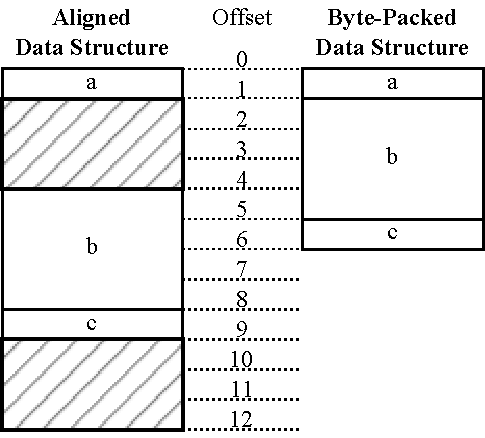
\includegraphics{Figures/AlignedVsPacked.pdf}
  \caption{Struct Byte-Packing.}
  \label{fig:aligned_vs_packed}
\end{figure}

\subsection{Basic Data Type Memory Layouts}

Having looked at the layout of members within a struct, another thing to consider is the layout of the basic data types themselves. \Gls{endianness} describes the \gls{byte} order of a multi-\gls{byte} basic data type. The two typical schemes are \gls{big-endian} and \gls{little-endian}. Take the $32$-bit value $\mathrm{AABBCCDD}_{16}$ as an example. Its \gls{big-endian} encoding corresponds to the following \gls{byte} layout in memory:
\begin{lstlisting}
  AA BB CC DD.
\end{lstlisting}
On the other hand, the \gls{little-endian} layout is:
\begin{lstlisting}
  DD CC BB AA.
\end{lstlisting}

While a detailed discussion of \gls{endianness} and the technical reasons for it is beyond the scope of this thesis there is an obvious design advantage to each of the two schemes just provided: With \gls{big-endian}, low-level debugging and the like is easier because the \gls{byte} order follows the natural reading layout. For \gls{little-endian}, value truncation may not require explicit instructions compared to \gls{big-endian}:

Take the example from above, i.e. the $32$-bit value $\mathrm{AABBCCDD}_{16}$. Now, we want to truncate it to a $16$-bit value, leaving us with $\mathrm{CCDD}_{16}$. We currently have a pointer to the $32$-bit value. For \gls{big-endian}, we can see that the $16$-bit value
\begin{lstlisting}
  CC DD
\end{lstlisting}
is at an offset of $2$ \glspl{byte} relative to the $32$-bit value. With \gls{little-endian}, the value
\begin{lstlisting}
  DD CC
\end{lstlisting}
is at an offset of $0$ \glspl{byte} relative to the $32$-bit value. Thus, \gls{little-endian} saves one arithmetic operation when retrieving the address of the truncated $16$-bit value compared to \gls{big-endian}. Today, most general-purpose \glspl{CPU} use the \gls{little-endian} layout, and \glsxtrshort{UEFI} currently mandates it~\cite{uefi-spec,ia32,arm-isa}. This leads to:

\begin{requirement}
  All basic types must be stored in the \gls{little-endian} layout.
\end{requirement}

\subsection{Signed Integer Encoding}

The \gls{twos-complement} is the standard choice for encoding signed integers for modern technologies. It is also the de facto standard for common general-purpose \glspl{ISA}~\cite{ia32,arm-isa}. Also, recent revisions of the \glsxtrshort{C} standard guarantee it as the only representation for its specified-width integer types~\cite{ISO:2018:III}.

Mathematically speaking, it is the positive complement in $\pmod 2^N$. It is well known that it holds that:
\begin{align*}
  \forall n,N \in \mathbb{N}_0. \quad -n \equiv 2^N - n \pmod{2^N}
\end{align*}
\begin{proof}
  $-n \equiv 2^N - n \Leftrightarrow 0 \equiv 2^N \Leftrightarrow 0 \equiv 0 \pmod{2^N}$
\end{proof}

$N$-bit integer arithmetic computes results $\bmod~2^N$ for addition, subtraction, and multiplication. The division operation is the regular integer division. In technical terms, the reduction $\bmod~2^N$ is commonly called an integer wraparound or integer overflow. Following the proposition above, it is easy to see that the same operator definitions apply to the \gls{twos-complement}.

For any positive number, one can easily compute the negative number of the same value by inverting all the bits and adding $1$. For example, for $-1$ and $N = 8$, we have:
\begin{align*}
   1_{10} &= 00000001_2,\\
  -1_{10} &= 11111111_{2C},\\
  11111111_{2} &= (2^8 - 1)_{10}.
\end{align*}

Historical alternatives to the \gls{twos-complement} were the \gls{ones-complement} and \gls{sign-and-magnitude}~\cite{ISO:2018:III}. Both include an explicit definition for $-0$ and arithmetic operations are not trivial to implement, e.g. \gls{ones-complement} addition requires an end-around-carry~\cite{1674817}. While other representations exist, they are not widely supported by general-purpose \glspl{CPU} and not supported by \glsxtrshort{UEFI}. This leads to:

\begin{requirement}
  All signed integers must be encoded as \gls{twos-complement}.
\end{requirement}

\subsection{Floating-Point Encoding}

For floating-point numbers, \glsxtrfull{IEEE}~754 is a well-established standard for both representation and computation rules~\cite{8766229}. While some hardware does not strictly follow the computational rules, and compilers them to be partially ignored for performance and efficiency reasons, the representation is de facto universal~\cite{gcc}. In fact, the \glsxtrshort{C} standard provides Annex F as a mapping of \glsxtrshort{C} floating-point types to IEEE-754 types, but not to any other encoding~\cite{ISO:2018:III}. This leads to:

\begin{requirement}
  All floating-point types must be encoded according to the \glsxtrfull{IEEE}~754 standard.
\end{requirement}

\subsection{Character and String Encodings}

The current standard for character encoding today is Unicode. It specifies several encoding formats, such as UTF-8 and UTF-16. The former is a strict superset of \gls{ASCII}, the traditional $7$-bit standard for control characters and the English alphabet, and is also widely used across different technologies~\cite{UCS}. \Glsxtrshort{UEFI} mostly uses UCS-2 encoding, which is a strict subset of UTF-16~\cite{uefi-spec,UCS}. For UCS-2, all characters occupy exactly $2$ \glspl{byte}. This allows many non-English characters to be represented but avoids the flexible-length parsing logic required by UTF-8. While UCS-2 is binary-incompatible with \gls{ASCII}, all UCS-2 characters representable by \gls{ASCII} can be converted to it by truncating to $7$ or $8$~bits~(bit 7 is always 0 for characters representable by \gls{ASCII}).

Besides Unicode, every recent alternative character set we have come across also extends \gls{ASCII}. Since localization is not an issue for a binary file format, \gls{ASCII} is sufficient as a de-facto universal standard character encoding.

For string encoding, we opt for zero-terminated \gls{ASCII} strings. Since \glsxtrshort{UEFI} primarily targets \glsxtrshort{C}, this is essential to harden the design against memory safety violations. Despite the availability of safe string functions that take an explicit size argument, \gls{EDK2} in particular often relies on zero-termination~\cite{edk2}. This leads to:

\begin{requirement}
  All characters must be encoded in the \gls{ASCII} format and all strings must be zero-terminated.
\end{requirement}

\section{Bit-Packing, Backward Compatibility, and Space Efficiency}
\label{sec:encoding_eff}

Space efficiency is one of the areas we are gradually improving over the existing \glsxtrshort{TE} format. To achieve this without sacrificing the flexibility of the \gls{image-file} format, we will now discuss various ways of compressing data while remaining portable and flexible.

\subsection{Bit-Packing in Image File Data Structures}

We refer to storing different values in a single datum as \gls{bit-packing} and to the result as a bit field. This is one of the simplest forms of compression. Using a boolean value as an example, a single \gls{byte} can store up to seven of them, one boolean state per bit, while boolean data types generally occupy at least $1$~\gls{byte}. Without further trickery, this is particularly useful and popular for so-called feature flags, which are boolean values that indicate support for a feature or a request for specific behaviour. See \Cref{sec:constr_packing} for sophisticated utilization of this paradigm.

There are two important operation classes for extracting values from bit fields. The first is the binary masking operator \texttt{AND}~($\&$). Masking refers to the character of the operands, as the operation applies bit-wise. The other is the binary shift operators left-shift~($\ll$) and right-shift~($\gg$). Rather than utilizing masks, their second operator is a `shift exponent'. The operations are identical to multiplying or dividing by $2^x$ respectively for their defined domain~(\glsxtrshort{C} prohibits shift exponents greater than or equal to the integer type's width). Compared to masks that affect specific bits at specific positions, the shift exponent affects the first operand's value as a whole.

To provide a minimum amount of backward compatibility, all unused bits must be declared as must-be-zero. This way, future specifications can use these bits to invoke new behaviour for non-zero values, without changing the semantics of old binaries.

\subsection{Utilizing Constraints for Compressed Encoding}
\label{sec:constr_packing}

In terms of \gls{image-file} formats, as we have seen, there are various constraints on metadata. For example, the \gls{data-alignment} requirement for \glspl{image-segment} must be a power of two. The most efficient encoding for this information is
\[ \mathsf{encode}(x) = \log_2(x). \]

By storing only the exponent, we can compress a $32$-bit \gls{image-segment} \gls{data-alignment} requirement to just its $5$-bit exponent. Decoding requires only a single binary operation:
\[ \mathsf{decode}(y) = 2^y = 1 \ll y. \]

Another example is that \glspl{image-segment} addresses and sizes must be aligned on this \gls{data-alignment} requirement boundary. There is no general requirement for its minimum. However, the \glsxtrshort{PE} format specifies a minimum of $512$~\glspl{byte}, and some operating systems reject \glspl{image-file} with an alignment less than the platform \gls{memory-page} size~\cite{pe-format,xnu,linux}. The following assumes an alignment of $4$~KiB.

The \gls{image-segment} addresses and sizes can be encoded as they are:
\[ \mathsf{encode}(x) = x, \]
but we know that
\[ x\bmod 4096 = x~\&~\mathrm{00000FFF}_{16} = 0, \]
which effectively frees the lower $12$~bits. When designating bits $[12 \twodots 31]$ in a $32$-bit word to the same bits of the address or size, a single binary operation is sufficient to decode either value:
\[ \mathsf{decode}(y) = y - y \bmod 4096 = y~\&~\mathrm{FFFFF000}_{16}. \]
The bits $[0 \twodots 11]$ can now be used for other purposes, such as feature flags. Semantically, this means that the bits $[12 \twodots 31]$ store the other factor to $4096$. The \glsxtrshort{PE} format uses this encoding for Base Relocation Blocks~(see \Cref{sec:pecoff}), which store their size in the low $12$~bits~\cite{pe-format}.

\subsection{Optimized Bit Field Layout}

For fixed-width integers, it is obvious to see that the worst-case number of masking bits is exactly the width of the type of the first operand. Meanwhile, the shift exponent only requires a logarithmic number of bits compared to the first operand. Thus, in general, shift operations are easier to encode in machine instructions and can result in shorter machine code~(see \Cref{fig:field_dec_sizes}). Of course, this still depends on the exact circumstances, including the target \gls{ISA}.

\begin{table}[htb]
  \centering
  \begin{tabular}{l c c c}
    \toprule
    \multirow{2}{*}[-2pt]{\textbf{Decoding}} & \multicolumn{3}{c}{\textbf{Code Size} [byte]}\\
    \cmidrule{2-4}
    & \textbf{x86-64} & \textbf{ARM64} & \textbf{RISC-V}\\
    \midrule
    Mask-Only & 29 & 40 & 28\\
    Shift-Only & 25 & 40 & 24\\
    \bottomrule
  \end{tabular}
  \caption{Bit Field Decoding Code Size Comparison.}
  \label{fig:field_dec_sizes}
  \caption*{Comparison of code sizes for mask-only and shift-only bit field decoding of two values across architectures. For the source data, see \Cref{sec:enc_formats}.}
\end{table}


Continuing the previous example of $4$~KiB alignment, some data structures can store both the address of a \gls{memory-page} and something related to indexing within it, such as an offset, a size, or a count of elements. For the \gls{memory-page} address, since the~(minimum) size for a given target architecture is usually known at build-time, one can factorize the value and store only the other factor, as seen before. When processing these data separately, it is more efficient to store the \gls{memory-page} address low and the other datum high, even if it is an offset and the opposite arrangement seems more natural~(see\Cref{sec:enc_formats}).

Flags are a special kind of bit field value because they only store boolean information. All that matters is whether the bit at the queried index is $0$ or $1$, which some architectures support checking in hardware~\cite{ia32}. Thus, they can be located anywhere in a bit field and always be evaluated with only a single \texttt{AND} instruction. However, especially when checking multiple flag bits that are located high at the same time, it may be beneficial to right-shift the bit field first and then test the bits with \texttt{AND} operations that now use shorter masks~(see \Cref{sec:flag_dec_opt}). Some \glspl{ISA}, as a result, allow for shorter instruction encodings for the \texttt{AND} operations~(see \Cref{fig:field_flag_dec_sizes}).

\begin{table}[htb]
  \centering
  \begin{tabular}{l c c c}
    \toprule
    \multirow{2}{*}[-2pt]{\textbf{Decoding}} & \multicolumn{3}{c}{\textbf{Code Size} [byte]}\\
    \cmidrule{2-4}
    & \textbf{x86-64} & \textbf{ARM64} & \textbf{RISC-V}\\
    \midrule
    Naive & 38 & 52 & 32\\
    Shift-Assisted & 37 & 44 & 32\\
    \bottomrule
  \end{tabular}
  \caption{Bit Field Decoding Code Size Comparison.}
  \label{fig:field_flag_dec_sizes}
  \caption*{Comparison of code sizes for naive and shift-assisted bit field decoding of three flags. For the source data, see \Cref{sec:flag_dec_opt}.}
\end{table}


In the absence of special optimizations, such as those above, it is generally best to arrange the bit field members in ascending order of size. This naturally reduces the values of the shift exponents. A convenient side effect is that the most significant member, which will be the largest value, does not require a masking operation for decoding.

\subsection{Relocation Fixup Table and Chains}
\label{sec:reloc_chains}

For the \gls{image-relocation}, we chose a delta encoding similar to dyld fixup chains~(see \Cref{sec:macho}). Replacing traditional \glspl{image-relocation-fixup} with their chained counterparts makes two assumptions:
\begin{enumerate}
  \item The \gls{image} does not need to run as-is, since storing metadata is inherently incompatible with having a valid target value.\label{asm:chain_1}
  \item The \gls{image} does not need to be relocated again, as applying a chained \gls{image-relocation-fixup} destroys its metadata, including the full index of the \gls{chained-image-relocation-fixups}.\label{asm:chain_2}
\end{enumerate}
\Glsxtrshort{RT} drivers violate Assumption~\ref{asm:chain_2} because after the operating system determines the \gls{virtual-memory} address mapping of the \glsxtrshort{UEFI} runtime memory, they may need to be relocated. This can be solved by indexing the \gls{image-relocation-fixup} table during the first load-time \gls{image-relocation} and using this index when relocating again for runtime execution. Due to time constraints, we simply disabled chained \glspl{image-relocation-fixup} for \glsxtrshort{RT} drivers and copy the \gls{image-relocation} table from the \gls{image-file}.

Pre-memory \glspl{PEIM} violate both Assumptions~\ref{asm:chain_1} and \ref{asm:chain_2}. Firstly, they must execute from the \gls{firmware} storage before the main memory is initialized. But they also need to be relocated in case they are shadowed~(this counts as a second \gls{image-relocation}, because the first time happened as part of the preloading at build-time). Due to Assumption~\ref{asm:chain_1}, we cannot store any metadata at the relocation target address and as such, so we need to disable chained \glspl{image-relocation-fixup} for pre-memory \glspl{PEIM}.

Similarly to \gls{chained-image-relocation-fixups}, the head fixup entries can be stored using delta encoding as well. For this, a fixup root entry stores the target address offset to the end of the previous \gls{image-relocation-fixup}. For the first fixup root entry, the previous reference address is always $0$. It is followed by a flexible array of head fixup entries that store the type of the current and the target offset of the next head reloc entry~(see \Cref{fig:ue_reloc_hierarchy}). In comparison to \glsxtrshort{PE}, which uses $4$-KiB-divided blocks, this technique can aggregate arbitrarily many head fixups under a single fixup root entry, so long as their offset is close enough. Like with \gls{chained-image-relocation-fixups}, our implementation allows offsets less than $4095$ \glspl{byte}. Effectively, the \gls{image-relocation} table becomes a nested singly-linked list~(see \Cref{fig:ue_reloc_org}).

\begin{figure}[htb]
  \centering
  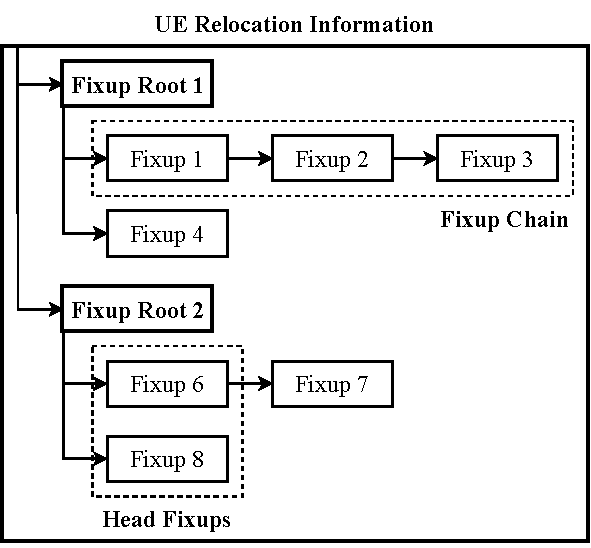
\includegraphics{Figures/UeRelocHierarchy.pdf}
  \caption{UE Relocation Information Logical Hierarchy.}
  \label{fig:ue_reloc_hierarchy}
  \caption*{The logical hierarchy of the \glsxtrshort{UE} relocation information. Fixup roots point to an area with one or more \glspl{image-relocation-fixup}. Head fixups are indexed within a fixup root and point to \gls{image-relocation} targets. These targets can, depending on the type, be the start of an \gls{image-relocation-fixup} chain, which is a singly-linked list of \gls{image-relocation} targets that technically resides outside the \gls{image-relocation} table.}
\end{figure}

\begin{figure}[htb]
  \centering
  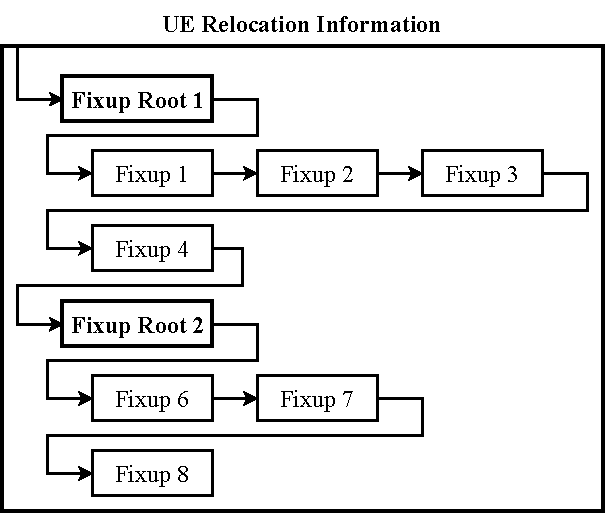
\includegraphics{Figures/UeRelocLinking.pdf}
  \caption{UE Relocation Information Technical Organization.}
  \label{fig:ue_reloc_org}
  \caption*{The technical organization of the \glsxtrshort{UE} relocation information. All data structures use delta encoding, i.e. they carry offsets to the end of the previous structure. Unlike the logical hierarchy~(see \Cref{fig:ue_reloc_hierarchy}), the technical organization is flat. This encoding is not only more space-efficient, but also forces all fixup roots, head fixups, and chained fixups to be disjoint and appear in ascending order by their target.}
\end{figure}

Furthermore, the \gls{image-relocation} target addresses --- this includes both \gls{chained-image-relocation-fixups} and non-chained head fixups --- are ordered ascending. As offset accumulation happens relative to the end of the previous \gls{image-relocation-fixup} for either kind~(see \Cref{fig:ue_reloc_enc}), this especially means that they are disjoint and that this can easily be verified in $O(n)$ while parsing the table. This could greatly benefit formalization or verification efforts, as the overall structure becomes much simpler and stricter. Verifying the correctness of deemed infeasible in the given timeframe when we verified a new implementation of the \gls{EDK2} \glsxtrshort{PE} loader~\cite{secure-pe}.

\begin{figure}[htbp]
  \centering
  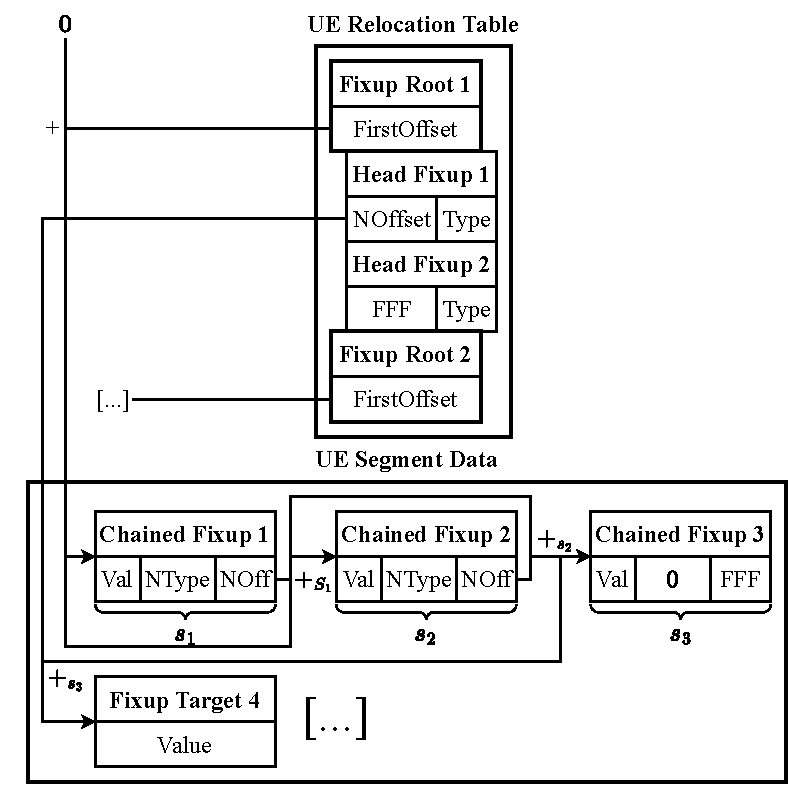
\includegraphics{Figures/UeRelocDetails.pdf}
  \caption{UE Relocation Information Delta Encoding.}
  \label{fig:ue_reloc_enc}
  \caption*{A more detailed illustration of the technical organization of the \glsxtrshort{UE} relocation information~(see \Cref{fig:ue_reloc_org}). Fixup roots carry the offset of their first head fixup. The offset of the first fixup root is relative to $0$~(so effectively absolute), while for the rest, it is relative to the end of the last \gls{image-relocation-fixup} in the previous fixup root. Head fixups store their type and the offset to the next head fixup from the end of the last \gls{image-relocation-fixup} in the current chain. Chained fixups store the type and relative offset of the next fixup in the chain, if any. An offset of $\mathrm{FFF}_{16}$ indicates that there are no more items in the fixup chain or the head fixup list. The offset of the next item accumulates continuously from the offset of the end of the previous item.}
\end{figure}

\subsection{Separating XIP Metadata from the Image Address Space}
\label{sec:ue_xip}

\Glsxtrshort{UEFI} \gls{XIP} \glspl{executable-file} reside on the \gls{firmware} storage. They are a special class of \glspl{executable-file} that must be executable without further modification, including \gls{image-file-loading} and \gls{image-relocation}. Techniques such as chained \gls{image-relocation-fixup} cannot be used, as they rely on storing metadata within the \gls{image} \gls{address-space}.

In particular, \gls{XIP} means that \glspl{image-segment} must be stored aligned, so the necessary padding must be stored explicitly. If adhering to the platform \gls{memory-page} size, this can be a significant overhead and can result in several kibibytes of padding. As \gls{firmware} storage is usually limited, the amount of aligned data should be kept to a minimum.

For the \glsxtrshort{PE} format, the \gls{image-file-header}, \gls{image-relocation} directory, and similar metadata are part of the \gls{image} \gls{address-space}. As such, they must be aligned by the \gls{image} alignment constraint. Since these metadata are not technically part of the \gls{image} and should always be read-only, they can be stored separately while preserving the general \gls{image} semantics.

So we propose separating the metadata from the \gls{image} \gls{address-space} completely. Compared to a non-\gls{XIP} \gls{image}, a \gls{XIP} \gls{image-file} should output two files:
\begin{itemize}
  \item The metadata file stores the \gls{image-file-header}, the \gls{image-relocation} table, the \gls{image} debug table, and other types of metadata. It only needs to be aligned regarding the general type \gls{data-alignment} constraints and should be protected with read-only \gls{memory-permissions}.
  \item The \gls{image} \gls{address-space} file stores the actual \gls{image} content. The \glspl{image-segment} may have interdependent references and as such they cannot be split. Therefore, to respect their potentially different \gls{memory-permissions}, they must be stored aligned on at least the platform \gls{memory-page} size boundary, as if the \gls{image} were loaded there.
\end{itemize}

The current \gls{FFS} design organizes \glspl{executable-file} in a flat manner, which prohibits us from implementing the above scheme~(see \Cref{sec:missing_features_archs}).

\section{Encoded Constraints, Simplified Parsing, and Loader Security}
\label{sec:encoding_sec}

Another important aspect of designing an \gls{image-file} format is to keep the data structures easy to parse. In fact, the safest parsing code is the one that does not exist. In this section, we will discuss how smart encoding can reduce the runtime parsing overhead and how to reduce the metadata that are exposed as part of an \gls{image} \gls{address-space}.

\subsection{Enforcing Constraints via Compressed Encoding}

If well-designed, the use of constraints for compressed encoding has a dual nature. Not only do the constraints enable the compression~(see \Cref{sec:constr_packing}), but the compression can also enforce the constraints.

Going back to the original example, the \gls{image} \gls{data-alignment} is ideally a multiple of the platform \gls{memory-page} size, as otherwise \gls{memory-permissions} cannot be applied~(see \Cref{sec:mem_perms}). While different platforms may have varying \gls{memory-page} sizes, \glsxtrshort{UEFI} effectively defines a minimum of $4$~KiB~\cite{uefi-spec}. Rather than testing whether the value is a multiple of $4$~KiB at runtime, we can enforce a constraint using the encoding scheme alone by storing
\[ \mathsf{encode}(x) = \log_2(\frac{x}{4096}) = \log_2(x) - 12. \]
This leaves us with a decoding operation of:
\[ \mathsf{decode}(y) = 2^y \cdot 4096 = 1 \ll (y + 12). \]

One more example is the \gls{memory-permissions} configuration. By good security practice, we want to enforce \gls{w-xor-x}~(see \Cref{sec:mem_wxorx}). With a typical read-write-execute bit field, this yet again requires a runtime check~\cite{audk}. However, let us take a look at all possible \gls{memory-permissions} configurations:
\begin{multicols}{2}
  \begin{enumerate}
    \item none \label{mem_perm_none}
    \item read \label{mem_perm_r}
    \item write \label{mem_perm_w}
    \item execute \label{mem_perm_x}
    \item read, write \label{mem_perm_rw}
    \item read, execute \label{mem_perm_rx}
    \item write, execute \label{mem_perm_wx}
    \item read, write, execute \label{mem_perm_rwx}
  \end{enumerate}
\end{multicols}

\begin{absolutelynopagebreak}
Using the \gls{w-xor-x} rule, we can immediately eliminate \Cref{mem_perm_wx,mem_perm_rwx}. Also, \Cref{mem_perm_none,mem_perm_w} are not useful in the context of \glspl{image-file}. This leaves us with:
\begin{multicols}{2}
  \begin{enumerate}
    \item read
    \item execute
    \item read, write
    \item read, execute
  \end{enumerate}
\end{multicols}
\end{absolutelynopagebreak}

As apparent, the amount of valid configurations is a power of two. This allows us to encode them using exactly $2$~bits by enumerating them. The resulting encoding prevents any violations of the \gls{w-xor-x} rule from being expressed, without involving runtime checks.

\subsection{Reimplementing HII Package List Exposure}

Due to the parsing burden on the \gls{module-dispatcher} and the overcomplicated structure of the \glsxtrshort{PE} resource directory, we propose a novel replacement for the current \glsxtrshort{UEFI-HII} package list storage. It must meet the following requirements:
\begin{enumerate}
  \item Due to the technical requirements of \glspl{IBV}, tools must be able to replace the \glsxtrshort{UEFI-HII} package list post-build~\cite{hii-mail}.
  \item Due to the implementation details of the \gls{EDK2} Shell, the \glsxtrshort{UEFI-HII} package list must be parsable at boot-time.
  \item To provide a significant security benefit over the current solution, the production code paths must not rely on parsing the \glsxtrshort{UEFI-HII} package list container.
  \item To provide a significant portability benefit, it should not rely on concepts that are not well established among the common \gls{executable-file} formats, \glsxtrshort{ELF}, \glsxtrshort{MACHO}, and \glsxtrshort{PE}.
\end{enumerate}

The layout of the data within \glspl{image-segment} depends on the \gls{image-linker} that composes it. However, given only a single datum, the common \gls{MSVC}, LLVM lld, and \glsxtrshort{GNU} ld \glspl{image-linker} will all produce an \gls{image-segment} with that datum located at the very beginning. This behaviour can be exploited by aggregating all \glsxtrshort{UEFI-HII} package list data into a single \glsxtrshort{C} struct, instantiating a global variable from it, and assigning it to a dedicated \gls{image-file-section}~(which will be the only \gls{image-file-section} of a dedicated \gls{image-segment}).

To meet the second requirement and to allow substitution of the \glsxtrshort{UEFI-HII} package list, which means its size cannot be known at build-time, we store it along with the data~(see \Cref{fig:new_hii_image}). This way, the size can be updated if the substituting \glsxtrshort{UEFI-HII} package list is larger or smaller than the one it replaces.

\begin{lstfloat}[htb]
  \centering
  \begin{lstlisting}[style=c]
typedef struct {
  UINT32                      Size;
  EFI_HII_PACKAGE_LIST_HEADER Header;
  //
  // UEFI HII package list data.
  //
} MODULE_HII_PACKAGE_LIST;
  \end{lstlisting}
  \caption{Data Structure for the UEFI HII Package List.}
  \label{fig:new_hii_image}
  \caption*{The data structure that encodes the \glsxtrshort{UEFI-HII} package list in a novel approach. Unlike the conventional \glsxtrshort{UEFI} solution, which uses the \glsxtrshort{PE}-specific resource directory that requires extra parsing, we utilize a regular \glsxtrshort{C} struct instance. To preserve the flexibility of the former method, the data structure is self-contained and forced into a dedicated \gls{image-segment} similarly to before.}
\end{lstfloat}

As we are guaranteed this data structure instance resides at the beginning of the designated \gls{image-segment}, the \glsxtrshort{UEFI-HII} package list can be located, parsed, and replaced with one that is at most the same size. To be able to replace it with a larger one, we force the designated \gls{image-segment} to be at the end of the \gls{image} \gls{address-space}. This allows us to grow and shrink it as required without affecting the rest of the \gls{image}.

This new model satisfies all the requirements we have been able to gather, without requiring any parsing from the \gls{module-dispatcher}.

\subsection{Image Debugging Information and Image Address Space}

The \glsxtrshort{PE} format has a unique property compared to the other \gls{image-file} formats. The \gls{image-file-header} is loaded at the \gls{image-base-address} and the first \gls{image-segment} starts after the \gls{image-file-header}. Other \gls{image-file} formats always load the first \gls{image-segment} at the \gls{image-base-address}, and if the \gls{image-file-header} is to be loaded, it must be part of the former. Since we generally do not want to load the \gls{image-file-header} into the \gls{image} \gls{address-space} at all, it must be removed during the conversion.

Consequently, when converting an \gls{image-file} to the new \gls{executable-file} format, the \gls{image-file} is first rebased to the \gls{image-base-address} minus the offset of the first \gls{image-segment} and then the \gls{image-base-address} is reset to the previous value. As a result, the \gls{image-file-header} has been removed from the \gls{image} \gls{address-space} without changing the \gls{image-base-address}.

For debugging, this means that the \gls{image-symbol} file will not match the newly converted file. For \glsxtrshort{ELF} and \glsxtrshort{MACHO} source files, the source file itself is the \gls{image-symbol} file and as such, they could also have the reserved area for the \gls{image-file-header} removed. However, for \glsxtrshort{PE} files, debug information is usually stored separately in a \gls{PDB} file~\cite{pdb-doc}, which is not trivial to rebase due to its proprietary nature~\cite{pdb-doc-deprecation}. As a workaround that works for all source \gls{image-file} formats, we store the stripped size along with the file path of the \gls{image-symbol} file~(see \Cref{{fig:ue_debug}}). When mapping the latter with a debugger, the \gls{image-base-address} is adjusted by said stripped size to account for the missing \gls{image-file-header}, so that the offsets of the \gls{image-segment} in the \gls{image} \gls{address-space} match again.

\begin{figure}[htb]
  \centering
  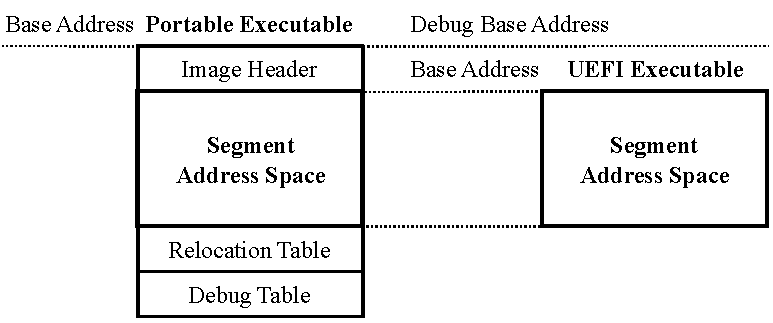
\includegraphics{Figures/UeDebug.pdf}
  \caption{UE Debug Model.}
  \label{fig:ue_debug}
  \caption*{The \glsxtrshort{UE} debug model. Compared to the source \glsxtrshort{PE} \gls{image}, \glsxtrshort{UE} does not map the \gls{image-file-header} and the metadata tables. While the latter does not cause any problems, as debugging is limited to symbolication and there can be no \glspl{image-symbol} targeting these tables, removing the \gls{image-file-header} will move all \glspl{image-segment} addresses. This can be accommodated with \glsxtrshort{ELF} or \glsxtrshort{MACHO} source files by relocating them, as they carry the \glspl{image-symbol}, but \glsxtrshort{PE} uses the proprietary \glsxtrshort{Microsoft} format \gls{PDB} for debugging. Since there is no easy way to update it with the new \gls{image-segment} addresses, \glsxtrshort{UE} can store a delta to the \gls{image-base-address} in the debug table. When symbolicating, this offset is applied and the \gls{PDB} is loaded so that the \glspl{image-segment} align.}
\end{figure}

\subsection{Discarding Load-Time Information}
\label{sec:reduce_info}

It is common for \glspl{image-file} to load their \gls{image-file-header} and debugging information into the \gls{image} \gls{address-space} --- for the \glsxtrshort{PE} format, the former is even done implicitly~\cite{pe-format}. This makes it easy to debug an \gls{image} by having all required data easily discoverable by memory traversal. However, this also has important downsides:
\begin{enumerate}
  \item This information occupies significant space, especially as all \glspl{image-segment} must be aligned at a \gls{memory-page} boundary.
  \item This information can be used by an operating system runtime attack on \glsxtrshort{RT} drivers to modify them with great reliability and predictability.
\end{enumerate}

Even for production builds, which have most of the useful debugging information stripped, the \glsxtrshort{PE} format requires loading the \gls{image-relocation} information into the \gls{image} \gls{address-space}~\cite{pe-format}. While it can be discarded safely after loading and linking have finished in theory, most notably the \gls{EDK2} \glsxtrshort{PE} \gls{image-file-loader} does not do this~\cite{edk2}.

In response, we have introduced a function at the \gls{API} level to discard information that is only needed at load-time~\cite{audk}. For \gls{PE} files, this overwrites the \gls{image-relocation} and \gls{image} debug tables with zero-values. Also, as a configuration option to the \gls{PE} loader, the \gls{image-file-header} area can be omitted. Finally, for \gls{image} debugging, we removed the assumption that the \glspl{image-symbol} file path is part of the \gls{image} \gls{address-space}. Instead, it is retrieved at load-time and stored as part of the central \glsxtrshort{UEFI} debug \gls{image} info table~\cite{uefi-spec}.

\chapter{Implementing UE Conversion and Loading}
\label{chap:uefi_exec_impl}

In this chapter, we will discuss the details of the implementation, which consists of a tool for \gls{image-file} format conversion, and the \gls{image-file-loader} \gls{library}. First, we will discuss the choice of an unstable design in \Cref{sec:unstable_design}. In \Cref{sec:loading_abstr}, we will explain how we used the \gls{image} abstraction to design a generic \glsxtrshort{UEFI} \gls{image} \gls{API}. Next, we will give a brief and high-level overview of the \gls{image-file-loading} process in \Cref{sec:algorithms}. In \Cref{sec:inter_rep}, we again use the \gls{image} abstraction to derive a new architecture for converting between \gls{image-file} formats. Finally, we describe how our \gls{image-file} conversion stack validates its outputs in \Cref{sec:out_validation}.

\section{Unstable Design and Scope Limitation}
\label{sec:unstable_design}

The proposed novel \glsxtrshort{UEFI} \gls{executable-file} format has a deliberately unstable design that is subject to change. This allows adjustments to be made during early adoption to accommodate previously unknown use cases without the technical debt resulting from backward compatibility. For many reasons, it may be desirable to preserve the unstable nature of the \gls{executable-file} format for \gls{firmware}-internal use. With the introduction of \gls{FCFI} mitigation support for the \glsxtrshort{PE} format, none of the intended ways of extensibility, such as the concept of data directories, was supported by \gls{EDK2} in a backwards-compatible manner. In response, the revised \glsxtrshort{PE} format designates a \glsxtrshort{PE} debug entry to expose the necessary metadata to support \gls{FCFI} mitigations~\cite{pe-format}. This results in unexpected semantics as the previous design designated these entries only for debugging, which typically requires only a single entry~\cite{edk2}.

However, for \gls{firmware}-internal images built from source, there is little reason to support backward compatibility, as they are rebuilt with each new revision of the \gls{firmware} image. This allows extending the unstable \gls{executable-file} format with new concepts as needed without having to define sophisticated abstractions for extensibility in advance.

\section{Image File Loading and Image Abstraction}
\label{sec:loading_abstr}

The \gls{image} abstraction is not only useful for \gls{image} generation but also \gls{image} loading. Here, the operations on the \gls{image} abstraction are most relevant.

\subsection{Generic UEFI Image File API}

Of course, in order not to break the \glsxtrshort{UEFI} boot specification and thus backward compatibility, we still need to support \glsxtrshort{PE} files. To avoid the burden of supporting \glsxtrshort{UE} and \glsxtrshort{PE} at the same time on the caller code, and to strengthen the \gls{image-file-loader} design, we have created a new, generic \gls{library} \gls{API}~\cite{thesis-git}. Like the design for \gls{image} generation, it is also based on the \glsxtrshort{UEFI} \gls{image} abstraction we defined~(see \Cref{sec:abstraction}), and it implements all the generic operations. Many of the metadata can be retrieved using getter functions. We have not abstracted the \gls{image-segment} and \gls{image-relocation} tables. Instead, we provide higher-level abstractions, such as retrieving an `\gls{image} record', which contains all the information necessary to apply \gls{memory-permissions} to an \gls{image} \gls{address-space}.

\subsection{Support for Multiple Image File Formats}
\label{sec:multi-format}

Using a generic \gls{API} for multiple \gls{image-file} formats means that each function needs to distinguish between them for any given reference object. To enable this, we have introduced generic context data structures for load-time and runtime contexts. These start with a format identifier that allows us to efficiently determine the \gls{image-file} format. Our implementation defines another, internal data structure that aggregates pointers to all format-specific \gls{library} and helper functions, which is statically instantiated for both \glsxtrshort{UE} and \glsxtrshort{PE}. The generic function implementations use a macro that implements an efficient decision for which of these data structures to use for format-specific calls. For further flexibility, it includes checks for build-time configuration options that define which \gls{image-file} formats are supported. We verified that with all modern toolchains\footnote{We tested \glsxtrshort{GCC} 11.3, Clang 16.0.6, Xcode 14.3, and \gls{MSVC} 2022 v17.6.2.}, the indirection via the internal data structures is optimized away when \gls{LTO} is enabled. The same is true for any support code for \gls{image-file} formats that have been disabled by said build-time configuration.

\subsection{Per-Source File Format Support}
\label{sec:multi-source}

As declared by the scope of the \glsxtrshort{UE} format, it is intentionally unstable and intended for \gls{firmware}-internal use, so only from the \gls{firmware} storage. Old \glsxtrshort{UE} binaries may remain structurally valid, but a new parser may interpret their semantics differently. This could lead to hidden security vulnerabilities. At the same time, some \glsxtrshort{UEFI-PI} and \glsxtrshort{UEFI} phases will only load \glspl{image-file} from the \gls{firmware} storage, such as \glsxtrshort{PEI} and \glsxtrshort{MM}. However, with a naive \gls{library} design, they would still carry the support code for \glsxtrshort{PE} files.

For these reasons, we have added configuration options to choose which \gls{image-file} formats are available from either the \gls{firmware} or external storage. For the scope of \glsxtrshort{UE}, this would mean that the \gls{firmware} storage would only carry \glsxtrshort{UE} files, while the external storage would only carry \glsxtrshort{PE} files. The caller specifies the source of the \gls{image-file} when initiating the parsing. As with the configuration of supported file formats on the \gls{library}-internal level~(see \Cref{sec:multi-format}), we have verified that \gls{LTO} optimizes the unreachable support code away. This solves both problems at once --- an attacker cannot introduce old \glsxtrshort{UE} binaries to the system to trigger exploitable behaviour, and the \glspl{module-dispatcher} that only handle \gls{firmware} \glspl{image-file} do not carry support code for both \gls{image-file} formats. Since the \glsxtrshort{DXE} phase deals with both sources, because it provides the image infrastructure for the \glsxtrshort{BDS} phase, it must inherently support both \gls{image-file} formats.

\pagebreak
\section{Algorithms for the UE File Format}
\label{sec:algorithms}

To illustrate the high-level \gls{image-file-loading} process, we provide some pseudocode descriptions for the main algorithms. While the first two algorithms are specific to the purposed \glsxtrshort{UE} file format, the last one is format-independent and part of the generic \gls{image-file-loader} \gls{library}.

\begin{algorithm}
  \caption{Loading a UE File.}
  \label{algo:load}
  \begin{algorithmic}[1]
    \Require{The \glsxtrshort{UE} file and a buffer to hold the \gls{image} \gls{address-space} as input.}
    \Ensure{The input buffer holds the \gls{image} \gls{address-space}.}
    \For{every \gls{image-segment}}
      \State Copy the \gls{image-segment} file contents.
      \State Zero the remaining \gls{image-segment} size.
    \EndFor
    \State Zero the remaining data of the input buffer.
  \end{algorithmic}
\end{algorithm}

\begin{algorithm}
  \caption{Relocating a UE File.}
  \label{algo:reloc}
  \begin{algorithmic}[1]
    \Require{The \glsxtrshort{UE} file, the \gls{image} memory, and the load address as inputs.}
    \Ensure{The \gls{image} has been relocated to execute from the load address.}
    \For{every fixup root}
      \For{every head fixup in the root}
        \For{every fixup in the chain}
          \State Apply the \gls{image-relocation-fixup}.
        \EndFor
      \EndFor
    \EndFor
  \end{algorithmic}
\end{algorithm}

\begin{algorithm}
  \caption{Setting up an Executable File for Execution.}
  \begin{algorithmic}[1]
    \Require{The \gls{executable-file} as input.}
    \Ensure{The \gls{executable-file} has been loaded and is ready to be executed.}
    \State Optionally hash~(e.g. execute \Cref{algo:dhash}) and authenticate the \gls{executable-file}.
    \State Parse the \gls{executable-file} and ensure structural correctness.
    \State Allocate enough read-write \glspl{memory-page} to hold the \gls{image} \gls{address-space}.
    \State Load the \gls{image}~(e.g. execute \Cref{algo:load}).
    \State Relocate the \gls{image}~(e.g. execute \Cref{algo:reloc}).
    \For{every \gls{image-segment}}
      \State Enforce the requested \gls{image-segment} \gls{memory-permissions}.
    \EndFor
    \State Flush the execution cache for the \gls{image} \gls{address-space}.
  \end{algorithmic}
\end{algorithm}

\FloatBarrier
\section{Image Generation and Image Abstraction}
\label{sec:inter_rep}

Like the current tooling used by \gls{EDK2} for some platforms, \glsxtrshort{UE} files should be generated from other \gls{image-file} formats. To do this, we use the previously defined \gls{image} abstraction to perform the conversion as such:
\begin{enumerate}
  \item Convert \glsxtrshort{ELF}, \glsxtrshort{MACHO}, \glsxtrshort{PE}, and \glsxtrshort{UE} \glspl{image-file} into the intermediate representation.
  \item Perform operations on the intermediate representation~(e.g. relocate the \gls{image}, or convert it into a \gls{XIP} \gls{image}).
  \item Convert the intermediate representation into an \glsxtrshort{UE} file.
\end{enumerate}

The proposed intermediate representation is a manifestation of the \gls{image} abstraction that we defined to make it easier to convert between specific \gls{image-file} formats~(see \Cref{fig:inter_rep} and \Cref{sec:abstr_data_structs}).

\begin{figure}[htb]
  \centering
  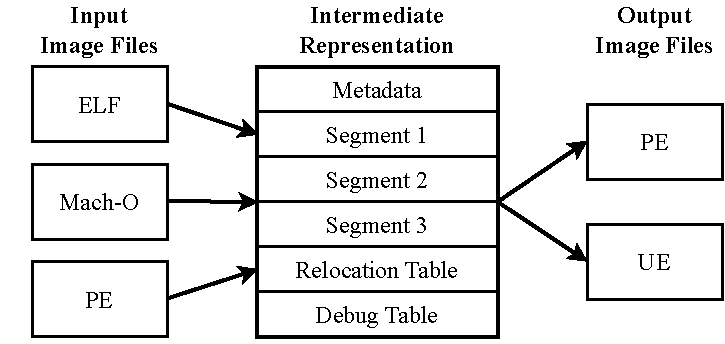
\includegraphics{Figures/InterRep.pdf}
  \caption{Image Intermediate Representation.}
  \label{fig:inter_rep}
  \caption*{The intermediate representation of an \gls{image}. We derived it from the data structures of the \gls{image} abstraction we defined earlier~(see \Cref{sec:abstr_data_structs}). The high-level idea is to instantiate an intermediate representation from input \gls{image-file}, allow generic operations to be performed on it~(e.g., \gls{image-relocation}), and finally to generate an output \gls{image-file} from it.}
\end{figure}

\section{Output Validation}
\label{sec:out_validation}

To reduce the testing overhead and the risk of exploitable translation bugs, we do as much output validation as possible at build-time as possible. Below we will look at the structural and semantic validation of the translation performed by our \gls{image-file} conversion stack.

\subsection{Conversion Equivalence Validation}
\label{sec:conv_eq}

As such, it can be used not only as an intermediate step during the conversion but also as an abstract representation of an \gls{image} in general. To take advantage of this ability to validate the equivalence of the input \gls{image-file} and the output \gls{image-file}, we propose to make the intermediate representation semi-canonical:
\begin{itemize}
  \item Most of the metadata is trivially canonical.
  \item \Glspl{image-segment} appear in ascending order by their address.
  \item \Gls{image-segment} sizes are multiples of the \gls{image} alignment.
  \item \Gls{image-segment} names are optional and may be omitted entirely. Even if they are not omitted, they may be truncated by the output conversion. The output name must be a prefix of the input name.
  \item Any \gls{image-relocation-fixup} that is not strictly necessary for \gls{image-relocation} is discarded.
  \item \Glspl{image-relocation-fixup} are converted to a universal format. To support all input file formats, only the least common denominator in terms of expressiveness is supported.
  \item \Glspl{image-relocation-fixup} appear in ascending order by their target address.
\end{itemize}

To validate the correctness of the conversation, we can compare the equivalence of the semi-canonical intermediate representations~(see \Cref{sec:inter_rep}) of the input file and the output file~(see \Cref{fig:img_conv_arch}). Since the intermediate representation is only semi-canonical, we cannot simply test for equality. In particular, for \gls{image-segment} names, which may be truncated or omitted, we check whether the name in the output file is a prefix of the name in the input file.

\begin{figure}[htb]
  \centering
  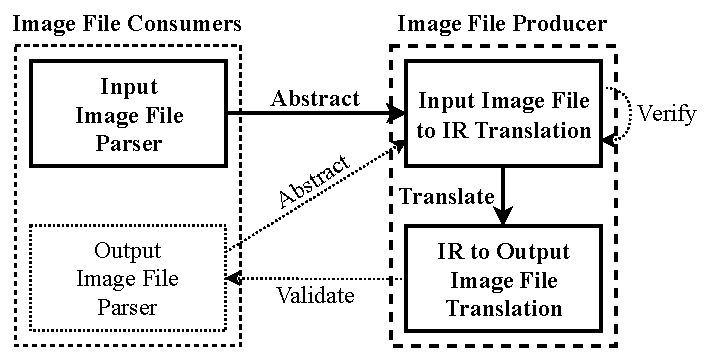
\includegraphics{Figures/ImageGenStack.pdf}
  \caption{Image File Conversion Architecture.}
  \label{fig:img_conv_arch}
  \caption*{The architecture of our \gls{image-file} conversion stack. First, the input \gls{image-file} parser is used to create the semi-canonical intermediate representation. Operations can now be performed on this intermediate representation. It is then translated into the output \gls{image-file}. This completes the conversion. To verify its correctness, the output file is parsed and abstracted into an intermediate representation. Using the semi-canonical properties, we then compare the input and output representations for equivalence.}
\end{figure}

\subsection{Format Constraint Validation}
\label{sec:constr_val}

In the past, malformed \glspl{image-file} have been shipped by various vendors~\cite{ipxe-fix,gnu-efi-fix}. The problems range from suboptimal configuration, such as too lax \gls{image-segment} \gls{data-alignment}, to violations of the \glsxtrshort{PE} specification, such as misaligned data structures. In order to combat such problems, extensive structural validation of all generated \glspl{image-file} must be performed. This should be done using the appropriate boot-time parsing \glspl{library} to ensure that the constraints are in sync with the consumer code.

For performance reasons, typical parsing \glspl{library} do not verify all requirements, including our proposed \glsxtrshort{UE} \gls{library} and the revised \glsxtrshort{PE} \gls{library}~\cite{secure-pe}. This may be because the constraint in question does not lead to unsafe behaviour if it is violated, e.g. the order of \glspl{image-relocation-fixup}. To account for this, we propose to support an optional flag to enable extensive structural validation. This must be disabled in production \gls{firmware} so as not to degrade performance, but debug \gls{firmware} may use it at the discretion of the platform maintainer. Most importantly, after generating an \gls{image-file} at build-time, it must be parsed with the extensive structural validation enabled, to ensure that it is well-formed and meets all the requirements of the consumer.

Reusing the parsing \gls{library} used at boot-time ensures that the producer code and the consumer code remain in sync. Note that if changes are made to the \gls{image} parsing code, the entire \gls{firmware} \gls{image} must be rebuilt to ensure that all \glspl{image-file} pass the extensive structural validation performed by the \gls{image-file} format conversion tool.

\chapter{Results and Discussion}
\label{chap:results}

Finally, we will evaluate our work. \Cref{sec:safety_val,sec:func_val,sec:space_eff_val} will cover our evaluation of the implementation's safety, functionality, and space efficiency, respectively. To conclude our work, we will outline our steps to enable artifact evaluation in \Cref{sec:repro}.

\section{Safety Validation}
\label{sec:safety_val}

To ensure the safety of our implementation, we have applied sophisticated analysis methods and performed extensive testing. While this cannot be guaranteed without the use of formal verification techniques, the goal is to ensure safety, especially memory safety in particular, for all conforming and malformed inputs. Due to time constraints, we focused only on \glsxtrshort{PE}-to-\glsxtrshort{UE} and \glsxtrshort{UE}-to-\glsxtrshort{UE} conversions for static analysis and \gls{fuzz-testing}. As such, both \glsxtrshort{ELF} input parsing and \glsxtrshort{PE} output generation have not been validated. We have also excluded \glspl{library} provided by the upstream \gls{AUDK} project from static analysis.

\subsection{Static Analysis}

For static analysis, we used GitHub CodeQL, Clang Static Analyzer, and Coverity. All three tools found valid bugs in both the upstream \gls{image-file} conversion tool and the support logic for the novel executable format. While we squashed fixes for the latter as development artifacts, we fixed the former in the $\mathrm{45440d1 \sim 4f49f08}$ commit range of our \gls{AUDK} fork~\cite{thesis-git}. The classes of valid bugs discovered were resource leaks and non-terminated strings~(not technically a bug, but a welcome precaution). We have never addressed nor inspected reported problems in underlying libraries from \gls{AUDK}. At the time of writing, no valid bugs in our implementation remain from the reports.

\subsection{Fuzz Testing}

We performed \gls{fuzz-testing} using LLVM libFuzzer~\cite{libfuzzer} and the existing OpenCore infrastructure for userland \gls{fuzz-testing}~\cite{opencore}. Two separate tools cover the parsing library and the conversion tool for the new \gls{executable-file} format, respectively~\cite{thesis-git}. In addition to the \gls{executable-file} input, the OpenCore \gls{fuzz-testing} infrastructure randomizes the global state for \gls{fault-injection} and platform configuration. To accomplish this, we reserve a configuration region at the end of the \gls{fuzz-testing} input.

OpenCore \gls{fuzz-testing} utilities share the trailer of the input data among the fuzz target input and the configuration region, as this allows to easily add legitimate, real-world inputs to the \gls{fuzz-testing} corpus. Testing the \glsxtrshort{PE} parsing library like this yielded good results, as the shared region corresponds to \glsxtrshort{PE} debug data that does not affect the control flow much. For the new \gls{executable-file} format, however, data is much more tightly-packed and there is little free-form data. To guarantee good results, we segmented the input data to strictly separate the fuzz target input from the global state configuration. To still use seed the \gls{fuzz-testing} corpus with real-world inputs, we developed a script that appends a global state region to them.

The initial state disables any \gls{fault-injection}, hence all of them should reach an overarching success path. The fuzzer can now mutate the global state configuration, the \gls{fault-injection} in particular, to trigger alternative and error paths, without altering the \gls{executable-file} portion of the input.

\Gls{fuzz-testing} discovered several safety violations, memory leaks, incorrect assertions, and unreachable code. These include the problems fixed by the commit range $\mathrm{45afac4 \sim 69b4dd1}$ of our \gls{AUDK} fork~\cite{thesis-git}. It achieved excellent code coverage metrics in the process~(see \Cref{fig:impl_cov}). We used $8$ workers per \gls{fuzz-testing} target for about two weeks and stopped the process when corpus mutation slowed down dramatically.

\begin{table}[!htb]
  \centering
  \begin{tabular}{l c c c}
    \toprule
    \multirow{2}{*}[-2pt]{\textbf{File}} & \multicolumn{3}{c}{\textbf{Coverage} [\%]}\\
    \cmidrule{2-4}
    & \textbf{Lines} & \textbf{Functions} & \textbf{Branches}\\
    \midrule
    UE Parsing & 100 & 100 & 100\\
    UE Conversion & 98.1 & 100 & 97.3\\
    \midrule
    \textbf{Total} & 98.8 & 100 & 98.1\\
    \bottomrule
  \end{tabular}
  \caption{UE Implementation Fuzz-Testing Coverage.}
  \label{fig:impl_cov}
  \caption*{Code coverage for the \gls{fuzz-testing} tools. For the source data, see \Cref{chap:code_cov}.}
\end{table}


\subsection{Fault Injection into Dynamic Memory Allocation}

To trigger all error handling paths, the OpenCore \gls{fuzz-testing} infrastructure performs \gls{fault-injection} on the \gls{EDK2} memory allocation library functions. At the time of writing, this is done via a  bitmap of width $64$. While bitmaps allow complex patterns to recur, the \gls{executable-file} format conversion tool aborts execution when \gls{dynamic-memory-allocation} fails. As such, failure patterns will not improve the path coverage of the fuzz target. At the same time, the width of the bitmap limits which allocations can be failed. As every allocation failure terminates the tool, at most $64$ applications can be failed by having exactly one bit cleared at a time. Due to the use of dynamically-growing buffers, more dynamic allocations may occur, however, they are unable to fail.

To address this issue, we propose a new modulo-based \gls{fault-injection} mode~\cite{thesis-git}. Instead of failing a \gls{dynamic-memory-allocation} when the bit that corresponds to its index is clear, it fails if its index $\bmod~N$ is equal to $N - 1$. This way, the fuzzer can increment the modulus to successively fail every individual dynamic allocation. This exponentially increases the maximum amount of \glspl{dynamic-memory-allocation} that can be failed compared to the bitmap approach. On the downside, it does not allow for \gls{fault-injection} patterns, but always fails every $N$-th \gls{dynamic-memory-allocation}. As every failure is fatal in our case, this does not cause any issues, though.

To be able to inject faults into every \gls{dynamic-memory-allocation}, the growing size of the dynamically-growing buffers was limited to $4$ \glspl{byte}, forcing frequent reallocations. Otherwise, it would be possible that certain operations could never realistically fail, as previous expansion operations would always allocate sufficient memory, but this is infeasible to prove and maintain.

\subsection{Fuzz Testing Feature Collisions and Fabrication}

While monitoring the progress of \gls{fuzz-testing}, we noticed that some error branches for \gls{dynamic-memory-allocation} were never hit, despite our best efforts to make them easy to fault one by one~(see \Cref{chap:code_cov})~\cite{thesis-git}. In an attempt to seed the corpus with such failure inputs, we manually fabricated a very large number of files with an incrementing fault modulus, which did indeed increase the coverage. However, when we tried to minimize the corpus, the new corpus again had no inputs that triggered these branches.

Although this is not easy to prove, we suspect that these paths were subject to feature collisions, i.e. they were classified as similar or identical to other inputs that did not trigger these branches~\cite{libfuzzer-coll}. The accuracy of \gls{fuzz-testing} code coverage is still an open research problem~\cite{8418631}. However, although they were not added to the corpus, libFuzzer probably generated and successfully processed inputs that triggered these branches.

In order to still trigger most of them with a reasonably sized corpus, we fabricated modules more efficiently~\cite{thesis-git}. We determined the module with the maximum number of \glspl{dynamic-memory-allocation}, hoping that it would hit most of the allocation paths, and fabricated exactly as many inputs that fault each allocation. As a result, the coverage of the corpus increased significantly but still did not cover all branches~(see \Cref{chap:code_cov}). However, as the fuzzer likely generated and processed inputs that hit them and the coverage data is otherwise excellent, we did not try to optimize the corpus further.

\section{Functional Validation}
\label{sec:func_val}

Of course, while safety and security are crucial to low-level software implementations, reliability and correctness are equally important. To validate the functionality of our implementation, we performed various kinds of manual and automated tests. In the following, we will discuss the functionality tests we performed regarding unit and system testing, as well as automated test case generation using \gls{fuzz-testing}.

\subsection{Unit Testing with Build Artifacts}
\label{sec:unit_tests}

To test the functionality of the conversion logic, we convert all \glspl{image-file} from \gls{OVMF} and \gls{ArmVirtQemu} across all supported architectures and targets from \glsxtrshort{PE} to \glsxtrshort{UE}. The correctness check of the output is part of the conversion procedure itself~(see \Cref{sec:conv_eq}) and does not require pre-computed outputs. This implicitly tests the correctness of most parts of the parsing library, as the correctness validation uses it for most parsing tasks~(see \Cref{sec:constr_val}). Rather than providing a separate test infrastructure for the remaining parts of the parsing library, future work should focus on deduplicating the unused parts of the parsing library as a first step~(see \Cref{sec:reloc_dedupe}).

\subsection{System Testing with Virtual Machines}

To test the functionality of the fully integrated system, we adapted the existing boot test infrastructure of \gls{AUDK}. We adjusted the \gls{OVMF} and \gls{ArmVirtQemu} platforms to use our novel \gls{executable-file} format for the \glsxtrshort{DXE}~(excl. \gls{EDK2}'s \textit{DxeCore}), \glsxtrshort{RT}, and \glsxtrshort{MM} stages. A script then performs automated tests with resulting \gls{firmware} \glspl{image} using the following environments~\cite{ocbuild}:
\begin{itemize}
  \item \textbf{TestConsole:} A simple \glsxtrshort{UEFI} application that prints `Hello World!' to the standard output console~\cite{ocbuild}.
  \item \textbf{TestLinux:} A minimal Linux 6.3 environment that performs basic platform initialization and then prints `Hello World!' to the standard output console~\cite{ocbuild}.
  \item \textbf{TestWindows:} A Windows 10 Preinstallation Environment that boots to a command prompt~\cite{ocbinarydata-winpe}.
\end{itemize}

Throughout development, we have had continuous automated testing of these scenarios using GitHub Actions \gls{CICD}.

\subsection{Automated Test Case Generation with Fuzz Testing}

The \gls{image-file} format conversion performs an internal check on the correctness of the translation output~(see \Cref{sec:conv_eq}). Thus, \gls{fuzz-testing} doubles as automated test case generation. The test tool will either reject an input if the input parser rejects it, or it will generate a correct translation. If the equivalence check fails, the tool asserts, which would classify the input as a crash during \gls{fuzz-testing}. However, due to the coverage-guided nature of libFuzzer, it is possible that most of the generated inputs were invalid and therefore rejected much earlier than to realistically stress-test the conversion equivalence logic.

\section{Space Efficiency Evaluation}
\label{sec:space_eff_val}

To compare the space efficiency of the newly-proposed \glsxtrshort{UE} format with the established \glsxtrshort{PE} solution, we generated both types of \glspl{executable-file} from the \gls{OVMF} and \gls{ArmVirtQemu} platforms across architectures and toolchains. Unlike unit tests~(see \Cref{sec:unit_tests}), \textit{OvmfIa32X64} was not considered because \textit{OvmfIa32} and \textit{OvmfX64} provide a superset of its \glspl{image-file}. We also only compared the \texttt{RELEASE} target, as it is the only one relevant to the production stage. Similarly, the \textit{CLANGPDB} toolchain was not considered, because it does not support compilation of \glsxtrshort{Arm} \glspl{image-file} and could therefore distort the final results between the architectures.

While the results are not groundbreaking, this is to be expected, as we focused mainly on optimizing the \gls{image-file-header} and the \gls{image-relocation} table, which are generally small compared to the size of the \glspl{image-segment}, especially without \gls{dynamic-linking}~(see \Cref{fig:rel_space_sav,fig:abs_space_sav,fig:tot_space_sav}). However, considering \gls{SPI} \gls{firmware} remains sparse and real-world platforms can be much more modular than \gls{OVMF} and \gls{ArmVirtQemu}, total platform space-savings of up to $78$~KiB are respectable. Once \gls{XIP} is implemented for \glsxtrshort{UE}~(see \Cref{sec:ue_xip}), we expect the results to improve significantly when comparing sizes on the final \gls{firmware} \gls{image}.

\begin{table}[htbp]
  \centering
  \begin{tabular}{l l l c c c}
    \toprule
    \multirow{2}{*}[-2pt]{\textbf{Platform}} & \multirow{2}{*}[-2pt]{\textbf{Arch}} & \multirow{2}{*}[-2pt]{\textbf{Toolchain}} & \multicolumn{3}{c}{\textbf{Saving} [\%]}\\
    \cmidrule{4-6}
     & & & \textbf{Min.} & \textbf{Avg.} & \textbf{Max.}\\
    \midrule
    \multirow{4}{*}[-2pt]{\gls{OVMF}} & \multirow{2}{*}{IA32} & GCC5 & 0.17 & 10.50 & 50.00\\
     & & CLANGDWARF & 0.17 & 10.66 & 53.75\\
    \cmidrule{2-6}
     & \multirow{2}{*}{X64} & GCC5 & 0.58 & 9.53 & 47.92\\
     & & CLANGDWARF & 0.60 & 10.09 & 47.83\\
    \midrule
    \multirow{4}{*}[-2pt]{\gls{ArmVirtQemu}} & \multirow{2}{*}{ARM} & GCC5 & 0.17 & 9.60 & 49.43\\
     & & CLANGDWARF & 0.17 & 8.70 & 50.60\\
    \cmidrule{2-6}
     & \multirow{2}{*}{AARCH64} & GCC5 & 0.60 & 9.52 & 54.41\\
     & & CLANGDWARF & 0.41 & 9.01 & 56.25\\
    \midrule
    \midrule
    \textbf{Average} & & & 0.36 & 9.70 & 51.27\\
    \bottomrule
  \end{tabular}
  \caption{Platform PE-to-UE Relative Space-Saving.}
  \label{fig:rel_space_sav}
  \caption*{Relagtive module space-savings from the \glsxtrshort{PE}-to-\glsxtrshort{UE} conversion per platform, architecture, and toolchain. All modules have been compiled in \texttt{RELEASE} mode. For the source data, see \Cref{chap:space_savings}.}
\end{table}


\begin{table}[htbp]
  \centering
  \begin{tabular}{l l l c c c}
    \toprule
    \multirow{2}{*}[-2pt]{\textbf{Platform}} & \multirow{2}{*}[-2pt]{\textbf{Arch}} & \multirow{2}{*}[-2pt]{\textbf{Toolchain}} & \multicolumn{3}{c}{\textbf{Saving} [byte]}\\
    \cmidrule{4-6}
     & & & \textbf{Min.} & \textbf{Avg.} & \textbf{Max.}\\
    \midrule
    \multirow{4}{*}[-2pt]{\gls{OVMF}} & \multirow{2}{*}{IA32} & GCC5 & 560 & 672.24 & 1,376\\
     & & CLANGDWARF & 536 & 669.80 & 1,384\\
    \cmidrule{2-6}
     & \multirow{2}{*}{X64} & GCC5 & 504 & 744.61 & 4,920\\
     & & CLANGDWARF & 432 & 758.93 & 4,960\\
    \midrule
    \multirow{4}{*}[-2pt]{\gls{ArmVirtQemu}} & \multirow{2}{*}{ARM} & GCC5 & 528 & 649.32 & 1,208\\
     & & CLANGDWARF & 552 & 666.64 & 1,376\\
    \cmidrule{2-6}
     & \multirow{2}{*}{AARCH64} & GCC5 & 472 & 753.00 & 4,952\\
     & & CLANGDWARF & 480 & 768.36 & 4,760\\
    \midrule
    \midrule
    \textbf{Average} & & & 508.0 & 710.36 & 3,117.0\\
    \bottomrule
  \end{tabular}
  \caption{Platform PE-to-UE Absolute Space-Saving.}
  \label{fig:abs_space_sav}
  \caption*{Absolute module space-savings from the \glsxtrshort{PE}-to-\glsxtrshort{UE} conversion per platform, architecture, and toolchain. All modules have been compiled in \texttt{RELEASE} mode. For the source data, see \Cref{chap:space_savings}.}
\end{table}


\begin{table}[htbp]
  \centering
  \begin{tabular}{l l l c c}
    \toprule
    \multirow{2}{*}[-2pt]{\textbf{Platform}} & \multirow{2}{*}[-2pt]{\textbf{Arch}} & \multirow{2}{*}[-2pt]{\textbf{Toolchain}} & \multicolumn{2}{c}{\textbf{Saving}}\\
    \cmidrule{4-5}
     & & & [KiB] & [\%]\\
    \midrule
    \multirow{4}{*}[-2pt]{\gls{OVMF}} & \multirow{2}{*}{IA32} & GCC5 & 66.96 & 2.64\\
     & & CLANGDWARF & 66.72 & 2.60\\
    \cmidrule{2-5}
     & \multirow{2}{*}{X64} & GCC5 & 76.35 & 2.63\\
     & & CLANGDWARF & 77.82 & 2.78\\
    \midrule
    \multirow{4}{*}[-2pt]{\gls{ArmVirtQemu}} & \multirow{2}{*}{ARM} & GCC5 & 53.90 & 2.79\\
     & & CLANGDWARF & 55.34 & 2.31\\
    \cmidrule{2-5}
     & \multirow{2}{*}{AARCH64} & GCC5 & 64.71 & 2.56\\
     & & CLANGDWARF & 66.03 & 1.87\\
    \midrule
    \midrule
    \textbf{Average} & & & 65.98 & 2.49\\
    \bottomrule
  \end{tabular}
  \caption{Platform PE-to-UE Total Space-Saving.}
  \label{fig:tot_space_sav}
  \caption*{Total space-savings from the \glsxtrshort{PE}-to-\glsxtrshort{UE} conversion per platform, architecture, and toolchain. All modules have been compiled in \texttt{RELEASE} mode. For the source data, see \Cref{chap:space_savings}.}
\end{table}


\section{Artifact Evaluation and Reproducibility}
\label{sec:repro}

To ensure the reproducibility of our results, we released a Docker~\cite{docker} container image~\cite{oci} with the development and testing environment used to produce all artifacts and to perform all tests~\cite{thesis-git}. Furthermore, we set up a GitHub Actions \gls{CICD}~\cite{gh-actions} infrastructure to automate artifact generation and all tests based on the existing \gls{AUDK} infrastructure. We used GitHub Actions \gls{CICD} to produce all discussed results, which did not involve self-hosted runners or proprietary code.

To increase confidence in the results, we also released a container description file that should continue to produce Docker images close to the image we provided. Unfortunately, bit-by-bit reproducibility is currently not a core feature of Docker and solutions like repro-get~\cite{repro-get} proved to be suboptimal for Ubuntu-based container base images. As a best-effort approach, we provide a Docker container image description that pinned all versions of all packages installed.

%%%%%%%%%%%%%%%%%%%%%%%%%%%%%%%%%%%%%%%%%%%%%%%%%%%%%%%%%%%%%%%%%%%%%%%%%%%%%%%
\chapter{Conclusion}
\label{chap:conclusion}

In order to significantly reduce the complexity of runtime parsing of \glsxtrshort{UEFI} \glspl{executable-file}, we have proposed a novel format that is strictly tailored to \glsxtrshort{UEFI} \gls{firmware} requirements. We have shown that files of our new format provide considerable space-saving when used for all platform modules, and their internal organization is visibly simpler compared to \glsxtrshort{PE}. In particular, it significantly extends the benefits of \glsxtrshort{TE} while retaining the expressiveness of \glsxtrshort{PE} in a \glsxtrshort{UEFI} context.

In addition, to make \gls{image-file} conversion easier to maintain, extend, and validate, we have implemented an approach based on an intermediate representation. This allows input and output formats to be processed independently of each other. At the same time, operations such as relocating an \gls{image} became format-independent, contributing to improved extensibility. Because we designed the intermediate representation to be semi-canonical, we were able to use it to reduce the validation of the output file to parsing the input file and comparing the resulting intermediate representation to the original one. With a small caveat, we did not encounter any malformed output files~(see \Cref{sec:reloc_dedupe}), as the conversion tool correctly aborted if the conversion was incorrect.

Finally, we applied static analysis and \gls{fuzz-testing} to our implementation. Due to the equivalence checking performed by the conversion procedure, the latter covered both safety and functional testing. After fixing the initial set of bugs, neither approach uncovered any new problems, and at the same time, we encountered no problems during real-world testing.

We subjected all results to artifact evaluation~\cite{thesis-git}. This includes pre- and post-conversion \glspl{executable-file}, \gls{AUDK} \gls{firmware} images for virtual machines, static analysis reports, and the \gls{fuzz-testing} corpora along with their code coverage. To further ensure reproducibility, GitHub Actions \gls{CICD} performed all tests using a semi-reproducible container. We have included both the container image used and the corresponding build description in the supplementary material.

All in all, we have solved the problems outlined in the problem statement and have empirically demonstrated the achievements in space efficiency and security hardening~(see \Cref{sec:problem_statement}).

\chapter{Future Work}
%%%%%%%%%%%%%%%%%%%%%%%%%%%%%%%%%%%%%%%%%%%%%%%%%%%%%%%%%%
\label{chap:future_work}

We would now like to discuss further improvements to our implementation that could be made in the future, as well as suggest ways to extend the core ideas to a larger scale.

\section{Missing Features and Architectures}
\label{sec:missing_features_archs}

For various reasons, even though we have solved the problem statement, we have not been able to provide all the features and compatibility one might expect. Below we will go through the shortcomings of our implementation and the reasons why we have not been able to address them.

\begin{itemize}
  \item \textbf{\gls{XIP}:} At this time, the planned \gls{XIP} mechanisms~(see \Cref{sec:ue_xip}) cannot be implemented, because the current \gls{EDK2} build system generates all \glsxtrshort{PE} files as \gls{XIP} and later stages rely on this fact. This is ensured by GenFw~(see \Cref{sec:genfw}). For \glsxtrshort{PE} files that do not meet \gls{memory-page} size alignment, the difference in space requirement is negligible, and the parser does not need to distinguish between \gls{XIP} and non-\gls{XIP}. As for the novel \gls{executable-file} format, we proposed a strict distinction, there is no good way to integrate \gls{XIP} support at this time. This implies that neither \glsxtrshort{SEC} nor \glsxtrshort{PEI} are currently supported.
  \item \textbf{DxeCore:} \Gls{EDK2}'s \textit{DxeCore} currently tries to re-parse its own \gls{image-file-header} to gather the information for \gls{image} \gls{address-space} memory protection. This works for \glsxtrshort{PE} files because their \gls{image-file-header} is always loaded implicitly into the \gls{image} \gls{address-space}. For the novel \gls{executable-file} format, we proposed to not do so~(see \Cref{sec:reduce_info}). The issue can easily be fixed by having \textit{PeiCore} pass the necessary information to \textit{DxeCore} via \glspl{HOB}. However, we did not implement this due to a novel patch to introduce memory protection into the \glsxtrshort{PEI} phase~\cite{pei-mem-perms}. Its introduction would implicitly resolve the issue.
  \item \textbf{RISC-V, LoongArch, \gls{FCFI}:} As we targeted the \gls{EDK2} fork \gls{AUDK}, we did not implement support for the RISC-V and LoongArch \glspl{ISA}, or for \gls{FCFI}, as \gls{AUDK} does not support any of them at the time of writing. Supporting the two \glspl{ISA} only requires porting their \gls{ISA}-specific \gls{image-relocation-fixup} to the novel \gls{executable-file} format, while \gls{FCFI} only requires translating a support flag, assuming \glsxtrshort{PE} support for all of them is added first.
\end{itemize}

\section{Deduplication of Image Relocation Table Parsing}
\label{sec:reloc_dedupe}

\Glspl{image-relocation-fixup} parsing can vary widely between \gls{image-file} formats, even if the high-level concepts are very similar. For this reason, it is not easy to provide an efficient abstraction for it. Unfortunately, this led us to duplicate the logic into the conversion tool, to not regress the performance and size of the parsing \gls{library}.

However, similarly to multi-format and multi-source support~(see \Cref{sec:multi-format,sec:multi-source}), we believe it might be possible to develop an abstraction \gls{API} that is well-optimized by the compiler. If that was feasible, the code duplication could be removed and the risk of deviating logic is removed. This would further strengthen the result of output equivalence checking~(see \Cref{sec:conv_eq}). Unfortunately, due to time constraints, we were unable to develop such an abstraction that satisfied our optimization criteria.

\section{Module Inter-Linking}

\Glsxtrshort{UEFI} continues to embrace a very modular architecture, factoring different functionalities into separate drivers, much like operating systems kernels do~(terminology may vary, e.g. for macOS they are called kernel extensions). However, \glsxtrshort{UEFI} and \gls{EDK2} in particular even separate security-critical components like the \glsxtrshort{CPU} abstraction used to apply \gls{memory-permissions} and generic platform policies like the supported \gls{image} authentication technologies~\cite{pi-spec,edk2}. The former makes \gls{EDK2} downstreams prone to load order-related bugs, the latter requires preserving \gls{API} stability for no particular reason~(and thus makes it hard to reuse an existing context structure that represents an \gls{image-file}, as the structure is subject to change). The obvious solution is to attempt to merge modules where beneficial.

\subsection{Static Linking, Pre-Ordering, and Events Listeners}

\Gls{static-linking} is the simplest technique for merging modules. One approach is to design modules as \glspl{static-library} and manually invoke their initialization routines as needed. Another approach is to utilize \gls{EDK2} library constructors as entry points and let the \gls{EDK2} build system automatically order the constructors according to the \gls{static-library} dependency lists.

The main disadvantage of using \gls{static-linking} is the reliance on \glspl{static-library}~(which are often just a collection of \glspl{object-file}). They are generally not cross-compatible with other compilers and sometimes not even between compiler versions. This introduces a dependency on the module vendor's build setup, whereas a separate driver is always interoperable.

Another issue that may require changes to the dependency's code is \gls{depex}. Since \glspl{PPI} and \glspl{uefi-protocol} can be installed at will, cross-dependencies are possible, and there is no general way to tell where a particular load order will satisfy each module's dependencies. Arguably, cross-dependencies are a bad design choice and it is not typical to use \gls{depex} to depend on \glspl{PPI} and \glspl{uefi-protocol} that are only installed on demand. By avoiding both and annotating each producer with the \glspl{PPI} or \glspl{uefi-protocol} it installs in its entry point, it is possible to compute a correct load order at build-time.

If the code cannot be changed, the behaviour of the \gls{module-dispatcher} can be mimicked using event listeners. With a \gls{PPI} or \gls{uefi-protocol}  installation notification. Once all dependencies are available, the entry point can be invoked.

\subsection{Prelinking and Composite Modules}
\label{sec:compmod}

To avoid the drawbacks of \gls{static-linking}, an interesting approach to \gls{dynamic-linking} can be considered. In the past, Apple shipped a full-fledged dynamic linker in its XNU kernel, called KXLD~\cite{xnu}. As \gls{dynamic-linking} can be a complicated process and both performance and security are valid concerns, they developed pre-linked kernel \glspl{image}. \Glspl{kernel-collection} are the latest iteration. The main instance is essentially a composite module of a kernel and many kernel extensions needed to boot~(see \Cref{fig:apple_kc}). The secondary instances, on the other hand, still depend on the main instance via pre-linking.

\begin{figure}[htb]
  \centering
  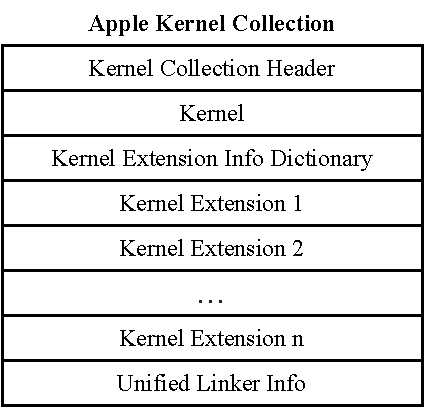
\includegraphics{Figures/AppleKC.pdf}
  \caption{Kernel Collection Executable File Format.}
  \label{fig:apple_kc}
  \caption*{A simplified overview of the \glsxtrshort{Apple} \gls{kernel-collection} format. It aggregates an operating system kernel and any number of kernel extensions into one, unified kernel collection \gls{executable-file}. The \gls{dynamic-linker} creates a wrapper \glsxtrshort{MACHO} \gls{image} that has the components shown above as \glspl{image-segment}. The kernel extension info dictionaries~(they contain information like which devices to attempt attaching to) are aggregated into one, unified kernel extension info dictionary~(also known as `prelink info'). The kernel and all kernel extensions of the \gls{kernel-collection} \gls{image} have their \gls{dynamic-linker} info~(e.g. \glspl{image-relocation-fixup}) aggregated into one, unified info \gls{image-segment} for the \gls{dynamic-linker}. This process does not require access to the source code or \glspl{object-file} of the involved modules.}
\end{figure}

The composition process involves merging both the \gls{image-segment} tables and the \gls{image-relocation} tables of all components. As this fixes the offsets between the kernel's \glspl{image-segment} and those of all its drivers, \gls{dynamic-linking} can be moved to the build-time by resolving the \glspl{image-symbol} and issuing \glspl{image-relocation-fixup} in return. The result essentially mimics \gls{static-linking}, except for features like \gls{image-segment} merging and \gls{LTO}. \Glsxtrshort{Apple} solved the former for the dyld shared cache, which consists of \gls{user-space} applications and \glspl{shared-library}, by issuing \glspl{image-relocation-fixup} for relative addressing.

In order for the kernel to be able to locate and start its drivers, the \gls{kernel-collection} contains a file with their locations and other metadata in a special \gls{image-file-section}. Unlike \gls{static-linking} with pre-ordering, locating and launching the dependency entry points is a runtime operation. However, this could be addressed by supporting the generation of an entry point stub that replaces the original entry point.

\section{Image File and Asset Digital Signing}

Since \glsxtrshort{UE} is currently only intended for \gls{firmware}-internal use, which generally does not require per-file authentication, we have not designed a working solution for it. However, if the new format proves to be useful, it may make sense to support it for external modules, such as \glspl{os-loader}. For this event, there are three possible ways to handle authentication.

\subsection{Appended Digital Signatures and File Prefix Hashing}

One way is to embed the \gls{digital-signature} in the \glspl{image-file}. For example, it can be appended to it~(see \Cref{algo:ehash})~\cite{pe-authenticode,linux-kmod-sig}. This is similar to how \gls{authcode} works, but collapses the hashing algorithm into a single step. This is done by storing the size of the unsigned \gls{image-file} in the \gls{image-file-header}, which is available at build-time. This is also the offset of the \gls{digital-signature}, if any, and its size is the size of the entire \gls{image-file} minus the stored offset. This does not require any modification to the \gls{image-file}, the \gls{digital-signature} is simply appended.

\begin{algorithm}
  \caption{Hashing an Image File With an Appended Digital Signature.}
  \label{algo:ehash}
  \begin{algorithmic}[1]
    \Require{The \gls{image-file}, a \gls{cryptographic-hash} function as input.}
    \Ensure{The \gls{image} \gls{cryptographic-hash} buffer has the \gls{image-file} \gls{digital-signature}.}
    \State \Gls{cryptographic-hash} the range $[0 \twodots \text{\lstinline{UnsignedSize}} - 1]$ of the \gls{image-file}.
  \end{algorithmic}
\end{algorithm}

\subsection{External Digital Signatures}

Another approach to storing \glspl{digital-signature} is externally from the file they sign. This is employed by \glsxtrshort{Apple} both for their \gls{firmware}-level and \gls{kernel-space}~(i.e. \glsxtrshort{Apple} Image4), as well user-space~(i.e. \glsxtrshort{Apple} application bundles) designs. The main advantages are that the signed file remains unchanged and that the filesystem takes over some parsing burden from the \gls{image-file-loader}. Depending on the cryptographic hashing algorithm, the signed file does not need to be parsed at all to authenticate it~(see \Cref{algo:dhash}).

\begin{algorithm}
  \caption{Hashing a UE File With an External Signature.}
  \label{algo:dhash}
  \begin{algorithmic}[1]
    \Require{The \gls{executable-file}, a \gls{cryptographic-hash} function as input.}
    \Ensure{The \gls{image} \gls{cryptographic-hash} buffer has the \glsxtrshort{UE} file \gls{digital-signature}.}
    \State Apply the \gls{cryptographic-hash} function to the entire \gls{executable-file}.
  \end{algorithmic}
\end{algorithm}

\subsection{Container Digital Signatures}

Similar to the embedded \glspl{digital-signature}, a container format could be specified where the \gls{digital-signature} is essentially prepended. This has the advantage that the signed data does not need to be parsed in any way prior to authentication. It can also be implemented as a generic format that is independent of the data being signed. Most importantly, it could be used for any asset that an \gls{image-file} might require and, in theory the authentication of the file could be part of loading the file from secondary storage. However, such standardization is rather unrealistic and using external \glspl{digital-signature} to collectively sign all assets in a database is likely to be more efficient and flexible.

\section{Self-Relocation}

\Gls{EDK2} for \glsxtrshort{Arm} architectures requires another concept that we have not yet covered --- self-relocation~\cite{edk2}. This is used for scenarios like TrustZone, where the hardware maps a module to a load address that is unknown at build-time. If this module has \glspl{image-relocation-fixup}, it must process them itself, as the hardware only maps the \gls{image-file}. It is critical that any code that runs until the \gls{image-relocation} has succeeded is not subject to \gls{image-relocation} and does not use any affected data.

There are currently no precautions in place to ensure a safe self-relocation process~\cite{edk2}. One way to help establish them is to identify all the code and data required for self-relocation and move them to dedicated \glspl{image-file-section}. With the critical components isolated, the \glspl{image-relocation-fixup} can be checked at build-time to ensure that they do not target any of them. Furthermore, when preserving the \gls{object-file} relocation fixups, which may contain sources of relative addressing, it can be checked that no critical component addresses a non-critical component. If both conditions are met, the self-relocation process is safe.

\section{Implementing Safety-Critical Code in Rust}

Despite the well-known caveats about using \glsxtrshort{Rust} for embedded development~(see \Cref{sec:rust-linux}), there are also organizational factors. First, \glsxtrshort{EDK2} is a much more corporate product than the Linux kernel. As a lot of development happens in proprietary environments that may not have a \glsxtrshort{Rust} development environment, and it may require formal requests to provide one. Also, a look at the corresponding mailing lists shows that the Linux kernel has much more development traffic than \glsxtrshort{EDK2}. The slow progress of proposals to add \glsxtrshort{Rust} support to \glsxtrshort{EDK2} is a clear indicator of both a lack of serious interest and possibly a lack of audience. \Gls{firmware} developers often have an electrical engineering background, which still resolves around \glsxtrshort{C}, and many may not be familiar with \glsxtrshort{Rust} or its novel concepts. For these reasons, we have chosen not to involve \glsxtrshort{Rust} in our implementation, in order to provide the easiest way to integrate our work into production \gls{firmware}.

Still, the strong guarantees of the \glsxtrshort{Rust} compiler would be a valuable addition to our stack of safeguards. While it is likely to be a long time before \glsxtrshort{Rust} properly enters the \gls{firmware} domain, we consider it to be a worthwhile investment on the road to memory safety.


%%%%%%%%%%%%%%%%%%%%%%%%%%%%%%%%%%%%%%%%%%%%%%%%%%%%%%%%%%%%%%%%%%%%%%%%%%%%%%%
% Biliography %%%%%%%%%%%%%%%%%%%%%%%%%%%%%%%%%%%%%%%%%%%%%%%%%%%%%%%%%%%%%%%%%

\printbibliography

%%%%%%%%%%%%%%%%%%%%%%%%%%%%%%%%%%%%%%%%%%%%%%%%%%%%%%%%%%%%%%%%%%%%%%%%%%%%%%%
% Appendix %%%%%%%%%%%%%%%%%%%%%%%%%%%%%%%%%%%%%%%%%%%%%%%%%%%%%%%%%%%%%%%%%%%%

\appendix

\chapter{My Code}

\blindtext[2]

\chapter{My Ideas}

\blindtext[2]

%%%%%%%%%%%%%%%%%%%%%%%%%%%%%%%%%%%%%%%%%%%%%%%%%%%%%%%%%%%%%%%%%%%%%%%%%%%%%%%

\end{document}
